% ============================================================
%  PFC — VERSÃO REVISADA
%  Este arquivo contém o documento COMPLETO (preâmbulo + capa +
%  ficha catalográfica + corpo + referências), pronto para
%  substituir o conteúdo do seu .tex no Overleaf.
%
%  Pontos de atenção marcados com comentários "%% NOTA:" ao
%  longo do texto indicam decisões que dependem de você
%  (ex.: sugestões de imagem, referências não verificadas).
% ============================================================
\documentclass[12pt, a4paper]{article}
\setlength{\headheight}{14.49998pt}

% ---- Pacotes ----
\usepackage[utf8]{inputenc}
\usepackage[T1]{fontenc}
\usepackage[brazil]{babel}
\usepackage{geometry}
\usepackage{setspace}
\usepackage{indentfirst}
\usepackage{xcolor}
\usepackage{mdframed}
\usepackage{tocloft}
\usepackage{titlesec}
\usepackage{fancyhdr}
\usepackage{hyperref}
\usepackage{booktabs}
\usepackage{longtable}
\usepackage{array}
\usepackage{graphicx}
\usepackage{float}
\usepackage{amsmath}
\usepackage{enumitem}
\usepackage{cite}
\usepackage{graphicx}
\usepackage{float}
\setlength{\parindent}{1.25cm}
\setlength{\parskip}{6pt}

% ---- Margens ABNT ----
\geometry{
  top=3cm,
  bottom=2cm,
  left=3cm,
  right=2cm
}

% ============================================================
%  CUSTOMIZAÇÃO DO SUMÁRIO
% ============================================================
\renewcommand{\contentsname}{Sumário}

\renewcommand{\cftsecfont}{\normalfont}
\renewcommand{\cftsecpagefont}{\normalfont}
\renewcommand{\cftsubsecfont}{\normalfont}
\renewcommand{\cftsubsubsecfont}{\normalfont}

\renewcommand{\cftsecleader}{\cftdotfill{\cftdotsep}}

\setlength{\cftbeforesecskip}{4pt}
\setlength{\cftbeforesubsecskip}{1pt}
\setlength{\cftbeforesubsubsecskip}{1pt}

\setlength{\cftsecindent}{0pt}
\setlength{\cftsubsecindent}{18pt}
\setlength{\cftsubsubsecindent}{36pt}

\setlength{\cftsecnumwidth}{24pt}
\setlength{\cftsubsecnumwidth}{28pt}
\setlength{\cftsubsubsecnumwidth}{36pt}

% ============================================================
%  FORMATAÇÃO DOS TÍTULOS DE SEÇÃO
% ============================================================
\titleformat{\section}
  {\normalfont\fontsize{12}{14}\selectfont\bfseries}
  {\thesection}{1em}{}

\titleformat{\subsection}
  {\normalfont\fontsize{12}{14}\selectfont}
  {\thesubsection}{1em}{}

\titleformat{\subsubsection}
  {\normalfont\fontsize{12}{14}\selectfont}
  {\thesubsubsection}{1em}{}

% ============================================================
%  CABEÇALHO COM NÚMERO DE PÁGINA
% ============================================================
\fancypagestyle{textual}{
  \fancyhf{}
  \fancyhead[R]{\thepage}
  \renewcommand{\headrulewidth}{0pt}
}

% ============================================================
\begin{document}
\pagestyle{empty}

% ============================================================
%  PÁGINA 1 — CAPA
% ============================================================
\begin{center}

  {\fontsize{12}{14}\selectfont\bfseries
    MINISTÉRIO DA DEFESA \\
    EXÉRCITO BRASILEIRO \\
    DEPARTAMENTO DE CIÊNCIA E TECNOLOGIA \\
    INSTITUTO MILITAR DE ENGENHARIA \\
    CURSO DE GRADUAÇÃO EM ENGENHARIA DE COMPUTAÇÃO
  }

  \vspace{6cm}

  {\fontsize{12}{16}\selectfont\bfseries
    JOÃO PEDRO BANDEIRA BELCHIOR \\[4pt]
    CARLOS ALEXANDRE SIQUEIRA DE ALMEIDA
  }

  \vspace{3cm}

  {\fontsize{12}{16}\selectfont\bfseries
    UTILIZAÇÃO DE INTELIGÊNCIA ARTIFICIAL \\
    PARA ANÁLISE E PROSPECÇÃO TECNOLÓGICA \\
    ATRAVÉS DA CONSULTA A ARTIGOS E PATENTES
  }

  \vfill

  {\fontsize{12}{16}\selectfont\bfseries
    RIO DE JANEIRO \\
    2026
  }

\end{center}

% ============================================================
%  PÁGINA 2 — FOLHA DE ROSTO
% ============================================================
\newpage

\begin{center}

  {\fontsize{12}{16}\selectfont\bfseries
    JOÃO PEDRO BANDEIRA BELCHIOR \\[4pt]
    CARLOS ALEXANDRE SIQUEIRA DE ALMEIDA
  }

  \vspace{4cm}

  {\fontsize{12}{16}\selectfont\bfseries
    UTILIZAÇÃO DE INTELIGÊNCIA ARTIFICIAL \\
    PARA ANÁLISE E PROSPECÇÃO TECNOLÓGICA \\
    ATRAVÉS DA CONSULTA À ARTIGOS E PATENTES
  }

  \vspace{3cm}

\end{center}

\hfill
\begin{minipage}{0.55\textwidth}
  \fontsize{12}{16}\selectfont
  Projeto de Final de Curso apresentado ao Curso de
  Graduação em Engenharia de Computação do Instituto
  Militar de Engenharia, como requisito parcial para a
  obtenção do título de Bacharel em Engenharia de
  Computação.

 \vspace{0.4cm}
Orientadora: Maria Cláudia Reis Cavalcanti, D.Sc.\\

Coorientadores externos:\\
Cel QEM José Adalberto França Junior -- AGITEC\\
Maj Giselle de Farias Rosa -- AGITEC
\end{minipage}
\vfill

\begin{center}
  {\fontsize{12}{16}\selectfont\bfseries
    RIO DE JANEIRO \\
    2026
  }
\end{center}

% ============================================================
%  PÁGINA 3 — FICHA CATALOGRÁFICA
% ============================================================
\newpage

\noindent
\textcopyright\,2026 \\
INSTITUTO MILITAR DE ENGENHARIA \\
Praça General Tibúrcio, 80 -- Praia Vermelha \\
Rio de Janeiro -- RJ\quad CEP: 22290-270

\vspace{1.2cm}

\noindent
Este exemplar é de propriedade do Instituto Militar de Engenharia, que poderá
incluí-lo em base de dados, armazenar em computador, microfilmar ou adotar
qualquer forma de arquivamento.

\vspace{0.6cm}

\noindent
É permitida a menção, reprodução parcial ou integral e a transmissão entre
bibliotecas deste trabalho, sem modificação de seu texto, em qualquer meio que
esteja ou venha a ser fixado, para pesquisa acadêmica, comentários e citações,
desde que sem finalidade comercial e que seja feita a referência bibliográfica
completa.

\vspace{0.6cm}

\noindent
Os conceitos expressos neste trabalho são de responsabilidade do(s) autor(es)
e do(s) orientador(es).

\vfill

\begin{mdframed}[
  linewidth=0.8pt,
  innerleftmargin=12pt,
  innerrightmargin=12pt,
  innertopmargin=10pt,
  innerbottommargin=10pt
]
  \fontsize{11}{14}\selectfont

  Bandeira Belchior, João Pedro; Siqueira de Almeida, Carlos Alexandre.

  \vspace{4pt}
  \quad\textit{Utilização de Inteligência Artificial para Análise e Prospecção
  Tecnológica Através da Consulta à Artigos e Patentes} / João Pedro Bandeira
  Belchior, Carlos Alexandre Siqueira de Almeida. -- Rio de Janeiro, 2026.

  \vspace{4pt}
  \quad 67 f.

  \vspace{4pt}
\quad Orientadora: Maria Cláudia Reis Cavalcanti.

\vspace{4pt}
\quad Coorientadores externos: José Adalberto França Junior; Giselle de Farias Rosa.

\vspace{4pt}
\quad Projeto de Final de Curso (graduação) -- Instituto Militar de
Engenharia, Engenharia de Computação, 2026.

\vspace{4pt}
\quad 1. Inteligência Artificial. 2. Prospecção Tecnológica. 3. Análise de
Patentes. 4. Processamento de Linguagem Natural. 5. Exército Brasileiro.
6. Recuperação Aumentada por Geração. 7. Modelos de Linguagem de Grande Escala.

\vspace{4pt}
\quad I. Reis Cavalcanti, Maria Cláudia (orient.) II. França Junior, José Adalberto (coorient. externo) III. Rosa, Giselle de Farias (coorient. externa) IV. Título

\end{mdframed}

% ============================================================
%  PÁGINA 4 — SUMÁRIO
% ============================================================
\newpage
\tableofcontents

% ============================================================
%  CORPO DO TEXTO
% ============================================================
\newpage
\pagestyle{textual}
\setcounter{page}{3}

% ============================================================
%  CAPÍTULO 1 — INTRODUÇÃO
% ============================================================
\section{Introdução}

  \subsection{Motivação}

  No contexto do desenvolvimento tecnológico, profissionais e técnicos envolvidos
em projetos de pesquisa e inovação frequentemente se deparam com um desafio
recorrente: a necessidade de identificar, avaliar e validar tecnologias
relevantes para suas áreas de atuação. Esse processo demanda um esforço considerável de busca em bases de dados de artigos científicos e registros de patentes \cite{rodriguezsalvador2017}, exigindo não apenas a localização das tecnologias pertinentes, mas também a verificação de sua atualidade --- isto é, se a produção científica sobre o tema permanece ativa e se a tecnologia já atingiu maturidade \cite{lezamanicolas2018}.

  A realização manual de um levantamento de prospecção tecnológica envolve,
em geral, múltiplas etapas de trabalho: a definição de termos de busca adequados
ao domínio investigado, a consulta a diferentes bases de dados com sintaxes e
interfaces distintas, a triagem de centenas ou milhares de resultados, a
verificação das instituições e pesquisadores mais relevantes no campo, a análise
das tendências de publicação ao longo do tempo e, por fim, a consolidação dessas
informações em um documento estruturado que possa subsidiar a tomada de decisão.
Cada uma dessas etapas, realizada de forma isolada e manual, consome horas ou
dias de trabalho de profissionais qualificados \cite{porter2004}.

  Esse trabalho consome tempo e recursos que poderiam ser direcionados às
etapas mais criativas e estratégicas do projeto. A ausência de ferramentas
integradas que automatizem esse fluxo de prospecção tecnológica representa um
gargalo significativo no ciclo de desenvolvimento de soluções inovadoras.
Adicionalmente, a qualidade do resultado depende fortemente da experiência do
pesquisador, da abrangência das bases consultadas e da consistência metodológica
adotada ao longo do processo --- fatores que introduzem variabilidade e risco de
viés nos levantamentos produzidos \cite{mayerhoff2008}.

  Diante desse cenário, surge a motivação para o desenvolvimento de uma
ferramenta baseada em Inteligência Artificial capaz de integrar-se a
\textit{Application Programming Interfaces} (APIs) de bases de patentes e
artigos científicos, realizando buscas direcionadas por meio de parâmetros-chave
fornecidos pelo usuário. O sistema propõe um ciclo iterativo de validação, no
qual o usuário refina progressivamente os critérios de busca, garantindo que os
resultados obtidos sejam relevantes e alinhados às necessidades do projeto em
questão. Esse ciclo iterativo, como será detalhado no Capítulo~2, é sustentado
em boa parte por técnicas de engenharia de \textit{prompt} --- a forma como o
sistema instrui os modelos de linguagem em cada etapa é, na prática, um dos
pilares estruturais da solução, e não um detalhe de implementação secundário,
razão pela qual lhe é dedicada uma seção própria da fundamentação teórica.

  Ao final desse processo, a ferramenta consolida as informações coletadas em um
relatório estruturado e editável, contendo os dados das patentes e artigos mais relevantes
sobre o tema, bem como as curvas~S que ilustram a evolução e o estágio de
maturidade das tecnologias identificadas. Com isso, o usuário é capaz de, a
partir da leitura de um único documento, inferir informações estratégicas
essenciais --- como o grau de consolidação de uma tecnologia, as tendências de
pesquisa mais recentes e as lacunas ainda existentes na literatura --- subsidiando
de forma eficiente e embasada a tomada de decisão para a incorporação dessas
tecnologias em seus projetos.

  \subsection{Caracterização do Problema}

  No âmbito do Exército Brasileiro, técnicos e engenheiros envolvidos em
projetos de Pesquisa, Desenvolvimento e Inovação (PD\&I) dedicam um tempo
significativo à busca manual de tecnologias em bases de artigos científicos e
registros de patentes relativas aos temas abordados nesses projetos. Além do
esforço de localização, é necessário verificar se essas tecnologias ainda estão
em desenvolvimento ativo --- tarefa igualmente trabalhosa e sujeita a
inconsistências quando realizada sem apoio de ferramentas adequadas.

  O problema central não se resume à simples busca de documentos. A dificuldade reside
em delimitar e consolidar, de forma coerente, informações provenientes de fontes
heterogêneas --- as diferentes APIs de patentes e artigos científicos possuem estruturas, campos,
metadados e síntese de busca distintas --- e transformar esses dados brutos em indicadores
estratégicos úteis: quais instituições lideram o desenvolvimento de uma
tecnologia, em que fase de maturidade ela se encontra, quais são as tendências
recentes de publicação e quais lacunas ainda permanecem em aberto na literatura.
Produzir esse panorama de forma confiável exige, além de esforço de pesquisa,
critério metodológico rigoroso e capacidade de síntese analítica \cite{porter2004}.

  Agravando esse cenário, as informações coletadas ao longo do processo
permanecem dispersas, sem um documento consolidado que permita ao responsável
pelo projeto extrair conclusões de forma rápida e confiável, e construir gráficos baseados nas fontes de pesquisa que estão sendo utilizadas. Essas
lacunas comprometem a qualidade das decisões e aumentam o risco de adoção de
tecnologias obsoletas ou redundantes, impactando diretamente a eficiência dos
projetos de defesa.

  Especificamente, as organizações que realizam pesquisa de tecnologias
emergentes enfrentam os seguintes desafios:

  \begin{itemize}
    \item A demanda em elaborar uma estratégia de busca coerente e sistemática, capaz de recuperar resultados mais fiéis, relevantes e alinhados aos objetivos da prospecção tecnológica.
    
    \item A necessidade de consolidar dados provenientes de múltiplas fontes
    heterogêneas (patentes e artigos científicos), cujas estruturas e campos
    diferem entre si, exigindo mapeamento e normalização antes de qualquer análise.

    \item A análise manual desses dados, que consome tempo e recursos humanos
    qualificados, sujeita a inconsistências e variações decorrentes da subjetividade
    do avaliador.

    \item A exigência de estrutura específica nos relatórios de prospecção, conforme
    os padrões REPTEC (\textit{Relatório de Prospecção Tecnológica}) e AGITEC
    (\textit{Agência de Gestão e Inovação Tecnológica}) \cite{agitec2024}, o que implica
    trabalho adicional de formatação e organização.

    \item A ausência de uma ferramenta integrada que combine, em um único fluxo
    automatizado, busca, análise e geração de relatórios.

    \item As limitações inerentes ao uso de APIs externas de busca científica e
    tecnológica: algumas exigem assinatura institucional ou chave de acesso, impõem
    limites ao número de resultados retornados por consulta, restringem os campos
    disponíveis para filtragem ou limitam a complexidade das consultas booleanas
    aceitas. Essas restrições precisam ser contornadas por estratégias de paginação,
    decomposição de consultas e tratamento de erros.

    \item O uso de Modelos de Linguagem de Grande Escala (LLMs) remotos pode oferecer
    qualidade textual elevada, mas implica custos recorrentes por \textit{token},
    limites de contexto e dependência de infraestrutura externa \cite{zhao2023},
    o que é problemático em contextos que exigem sigilo e controle de dados sensíveis.
    Já os modelos locais reduzem esses riscos, mas impõem requisitos computacionais
    que podem ser incompatíveis com máquinas comuns.

    \item A geração automática de relatórios por LLMs está sujeita ao fenômeno de
    alucinação \cite{ji2022}, no qual o modelo produz informações plausíveis, porém
    factualmente incorretas. A adoção de técnicas como \textit{Retrieval-Augmented
    Generation} (RAG) e a manutenção de etapas de validação humana são essenciais
    para mitigar esse risco.
  \end{itemize}

  Existe, portanto, um compromisso permanente entre qualidade, custo, privacidade
e desempenho que precisa ser gerenciado ao longo de todo o projeto. Modelos
remotos tendem a ser mais precisos e rápidos, porém dependem de limites externos
e apresentam custo recorrente \cite{brown2020}. Modelos locais garantem controle
e privacidade, mas podem ser mais lentos e menos precisos, especialmente em
tarefas que exigem geração de texto técnico em português formal.

  \subsection{Objetivo}

    \subsubsection*{Objetivo Geral}

  O objetivo geral do presente projeto é o desenvolvimento de um sistema
inteligente baseado em Inteligência Artificial para automatizar o processo de
prospecção tecnológica, por meio da consulta integrada a bases de artigos
científicos e patentes, da análise dos resultados recuperados e da geração
automática de um relatório técnico consolidado no padrão estabelecido pela
AGITEC \cite{agitec2024}.

    \subsubsection*{Objetivos Específicos}

  Para a consecução do objetivo geral, estabeleceram-se os seguintes objetivos
específicos:

  \begin{enumerate}[label=\roman*.]
    \item Promover a integração com modelos de linguagem selecionados pelo usuário --- remotos, como as famílias Claude, da Anthropic, e Gemini, do Google, ou locais, executados por meio da plataforma Ollama ---, configuráveis individualmente para cada ponto de uso do sistema, de modo a viabilizar a geração assistida de estratégias de busca mais coerentes, estruturadas e aderentes ao tema investigado, a partir dos parâmetros fornecidos pelo usuário.
    \item Integrar o sistema às APIs \textit{Open Patent Services} (OPS) do
    Escritório Europeu de Patentes (EPO), Scopus da Elsevier e às bases Lens Patents e Lens Scholarly,
da plataforma Lens, viabilizando a
    recuperação automatizada de patentes e artigos científicos a partir de
    parâmetros fornecidos pelo usuário.

    \item Implementar módulos de construção de consultas (\textit{query builders})
    capazes de transformar termos de busca em consultas estruturadas, compatíveis com
    a sintaxe de cada API, incluindo o uso de operadores booleanos, filtros
    temporais e campos específicos.

    \item Desenvolver um mecanismo de geração e refinamento de termos e consultas
    de busca por meio de LLMs, combinado a um pipeline de
    processamento de linguagem natural local para extração e pontuação de
    termos candidatos a partir dos resultados exploratórios, de modo a ampliar
    a cobertura temática e garantir a qualidade das consultas submetidas às
    APIs externas.

    \item Implementar um ciclo iterativo de validação humana que permita ao usuário
    aprovar, ajustar ou rejeitar os termos e consultas gerados pelo modelo antes da
    execução das buscas definitivas.

    \item Consolidar os metadados heterogêneos retornados pelas diferentes APIs
    em um formato interno unificado, realizando agregações por ano, por depositante
    ou instituição, e por classificação tecnológica ou área de estudo, utilizando técnicas de inferência estatística, a fim de subsidiar a análise de tendências.

    \item Calcular automaticamente a fase de maturidade tecnológica de Ernst da área
    pesquisada com base na taxa de crescimento das publicações e patentes
    recuperadas, gerando a representação gráfica da curva~S correspondente.

    \item Gerar automaticamente um relatório técnico consolidado no formato
    REPTEC/AGITEC, editável, com embasamento factual garantido pelo uso de técnicas de
    Geração Aumentada por Recuperação (RAG), a partir dos
    documentos indexados no banco vetorial.

    \item Persistir de forma estruturada e rastreável os dados gerados ao longo
    do processo de prospecção, distribuindo-os entre diferentes sistemas de
    armazenamento conforme sua natureza: um banco de dados relacional
    (PostgreSQL) para os metadados estruturados de sessões, consultas,
    documentos de patente e artigo recuperados, e histórico de execução; um
    banco de dados vetorial (ChromaDB) para os \textit{embeddings} utilizados
    na recuperação semântica via RAG; e um serviço remoto de armazenamento de
    objetos (MinIO) para os artefatos gerados, como os gráficos da curva~S e o
    relatório final.

    \item Desenvolver uma interface \textit{web} para acompanhamento e auditoria do processo
    de prospecção, para edição do relatório gerado e exportação do documento final, e verificação de dados estatísticos acumulados de pesquisas realizadas ao longo do tempo, como custos, tempo de processamento etc.
  \end{enumerate}

  \subsection{Metodologia}

  O sistema proposto implementa um fluxo iterativo de prospecção tecnológica
baseado em Inteligência Artificial, estruturado em torno de duas frentes paralelas e
independentes: a busca em bases de patentes e a busca em bases de artigos
científicos. Ambas seguem o mesmo ciclo de execução.

  O processo se inicia com o fornecimento de parâmetros pelo usuário por meio
de uma interface \textit{web} dedicada: a etapa de intake é a primeira etapa do mesmo \textit{wizard} que conduz
o usuário por todo o fluxo de prospecção. A partir dessas entradas, o modelo de linguagem remoto escolhido, direcionado por técnicas de engenharia de prompt, gera um conjunto
de variações temáticas relacionadas ao tema informado, que são apresentadas ao usuário
para validação \cite{white2023}. Nessa etapa, o usuário pode aprovar o tema,
solicitar maior especificidade ou alterá-lo diretamente antes de prosseguir.

  Com o tema validado, o sistema realiza uma busca exploratória inicial nas APIs selecionadas para patentes e artigos, utilizando a linguagem de consulta CQL
(\textit{Common Query Language}) no caso do OPS, e a sintaxe própria de campos no
caso do Scopus, recuperando um
conjunto preliminar de resultados. Os títulos e resumos desses resultados são então processados por um
pipeline local de Processamento de Linguagem Natural (PLN) -- e não por uma nova chamada ao modelo de
linguagem remoto -- que extrai e pontua os termos mais relevantes, apresentados ao
usuário para seleção. Com os termos selecionados, o modelo de linguagem remoto constrói,
a partir deles, opções de \textit{queries} refinadas para a
busca definitiva, novamente submetidas à validação do
usuário, que deve selecionar uma opção ou retornar aos valores anteriores, podendo solicitar ajustes.

  Após a aprovação, o sistema executa a busca final e recupera o conjunto
definitivo de patentes e artigos. Os dados coletados alimentam, por um lado, o
cálculo automático das curvas~S da tecnologia pesquisada (Seção~\ref{sec:curva-s}) e,
por outro, a indexação, em um
banco de dados vetorial (ChromaDB), do título e do resumo dos documentos
recuperados na busca final, por meio da técnica de RAG
(\textit{Retrieval-Augmented Generation}) \cite{lewis2020, gao2024}, que
permite a um modelo de linguagem local gerar conteúdo factualmente embasado
nos documentos recuperados, minimizando a ocorrência de alucinações
\cite{ji2022}. A aderência ao padrão REPTEC/AGITEC é garantida por um
\textit{template} LaTeX e por seções de texto fixo extraídas de um relatório
real \cite{reptec2023tetra}. Com esses dados, é gerado automaticamente um
relatório consolidado em LaTeX, contendo os gráficos da análise, as
referências efetivamente citadas e o quadro com as consultas de busca
utilizadas, que o usuário pode editar, revisar e compilar em PDF diretamente
na interface \textit{web}.

  \subsection{Estrutura do Texto}

  O presente trabalho está organizado em mais cinco capítulos. O
\textbf{Capítulo~2} aborda a fundamentação teórica necessária à compreensão do
sistema desenvolvido, tratando de prospecção tecnológica, curva~S de maturidade
tecnológica (e sua distinção em relação ao conceito de \textit{Technology Readiness
Level}), \textit{Large Language Models} (LLMs) e as redes neurais em que se
baseiam, engenharia de \textit{prompt} --- técnica que perpassa praticamente todas
as etapas do \textit{pipeline} e que, por isso, recebe tratamento aprofundado ---,
\textit{Retrieval-Augmented Generation} (RAG), \textit{embeddings}, bancos de
dados vetoriais e as principais APIs e ferramentas utilizadas. O \textbf{Capítulo~3} apresenta
a solução proposta: escopo, requisitos funcionais e não funcionais, especificação
da arquitetura (incluindo a arquitetura hexagonal e os princípios SOLID que a
sustentam), configurações e parâmetros adotados, tecnologias empregadas e estado
atual de desenvolvimento. O \textbf{Capítulo~4} detalha o
\textit{pipeline} de processamento em suas cinco fases. O \textbf{Capítulo~5}
apresenta o cronograma de desenvolvimento do projeto. O
\textbf{Capítulo~6} traz as considerações finais, os resultados esperados e as
limitações identificadas.

% ============================================================
%  CAPÍTULO 2 — FUNDAMENTAÇÃO TEÓRICA
% ============================================================
\section{Fundamentação Teórica}

  \subsection{Prospecção Tecnológica}

  A prospecção tecnológica é um conjunto de métodos e ferramentas utilizado para
identificar, analisar e monitorar tecnologias emergentes e suas tendências de
desenvolvimento \cite{porter2004}. Seu objetivo é fornecer subsídios para a tomada
de decisão estratégica em organizações de pesquisa, desenvolvimento e inovação,
permitindo antecipar oportunidades e riscos associados à adoção de novas
tecnologias. Segundo Mayerhoff \cite{mayerhoff2008}, o propósito dos estudos de
prospecção não é desvendar o futuro, mas sim delinear e testar visões possíveis
e desejáveis para que sejam feitas, hoje, escolhas que contribuirão da forma mais
positiva possível na construção do futuro.

  No contexto brasileiro de defesa, essa atividade é formalizada por meio dos
padrões REPTEC da AGITEC, que estabelecem estrutura, conteúdo mínimo e formato
para relatórios de prospecção tecnológica utilizados pelo Exército Brasileiro
\cite{agitec2024}. Um exemplo concreto e público dessa formalização é o
Relatório de Prospecção Tecnológica 001/2023, elaborado pela AGITEC sobre a
tecnologia \textit{Terrestrial Trunked Radio} (TETRA) \cite{reptec2023tetra},
que segue a estrutura em oito seções (Finalidade, Referências, Objetivo,
Introdução, Metodologia, Resultados, Conclusão e Referências Bibliográficas) e
emprega, nas subseções de Resultados, exatamente o tipo de indicador
bibliométrico -- distribuição temporal de publicações e patentes, \textit{ranking}
de instituições e depositantes, classificações CPC mais frequentes e curvas de
extrapolação -- que o sistema aqui descrito busca automatizar. Tais relatórios
devem contemplar, entre outros elementos,
análise de patentes, levantamento de artigos científicos, análise de tendências
e representação gráfica do ciclo de vida das tecnologias investigadas. O
cumprimento desses padrões exige que os dados coletados sejam organizados em
seções específicas, como finalidade, referências institucionais, metodologia de
busca, informações científicas e tecnológicas, tendências e ciclo de vida, e
conclusão embasada nos dados apresentados.

  A utilização de artigos científicos e patentes como fontes primárias de
informação tecnológica é amplamente reconhecida na literatura \cite{porter2004}.
Artigos científicos refletem o estado do conhecimento acadêmico e são indicadores
do avanço teórico e experimental em um campo, geralmente associados aos estágios
iniciais do ciclo de vida de uma tecnologia, quando a pesquisa básica e aplicada
ainda predomina sobre a exploração comercial. Patentes, por sua vez, revelam
tendências de inovação industrial e comercial, identificando as organizações
mais ativas no desenvolvimento tecnológico, os inventores de destaque e as
classificações tecnológicas predominantes, e tendem a acompanhar estágios de
maturidade mais avançados, em que o interesse comercial pela proteção de
propriedade intelectual se intensifica \cite{reptec2023tetra}. A análise combinada dessas duas fontes
oferece, portanto, uma visão mais abrangente e multidimensional do panorama
tecnológico de um tema --- é exatamente essa complementaridade entre "perfil
científico" e "perfil tecnológico" que justifica, no sistema desenvolvido, a
manutenção de duas frentes de busca paralelas e independentes (OPS/Lens
Patents para patentes, Scopus/Lens Scholarly para artigos), em vez de uma
fonte única.

\begin{figure}[H]
    \centering
    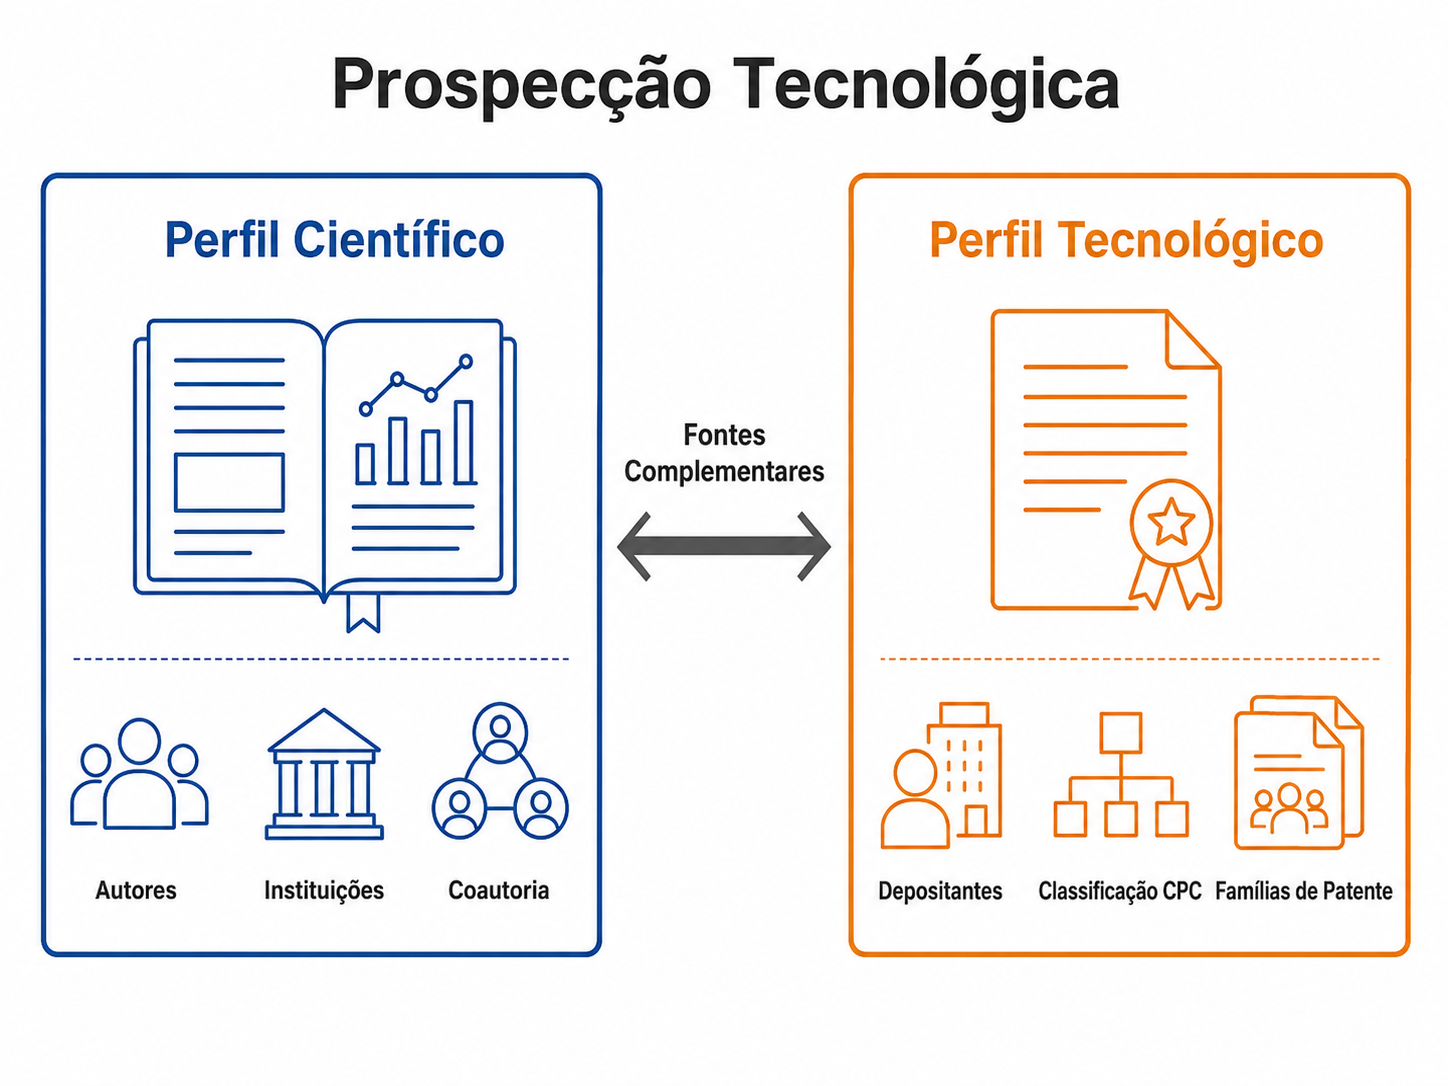
\includegraphics[width=0.5\textwidth]{img/perfil_cientifico_tecnologico.png}
    \caption{Perfil científico e perfil tecnológico como fontes complementares de prospecção.}
    \label{fig:perfil-cientifico-tecnologico}
\end{figure}

\begin{figure}[H]
    \centering
    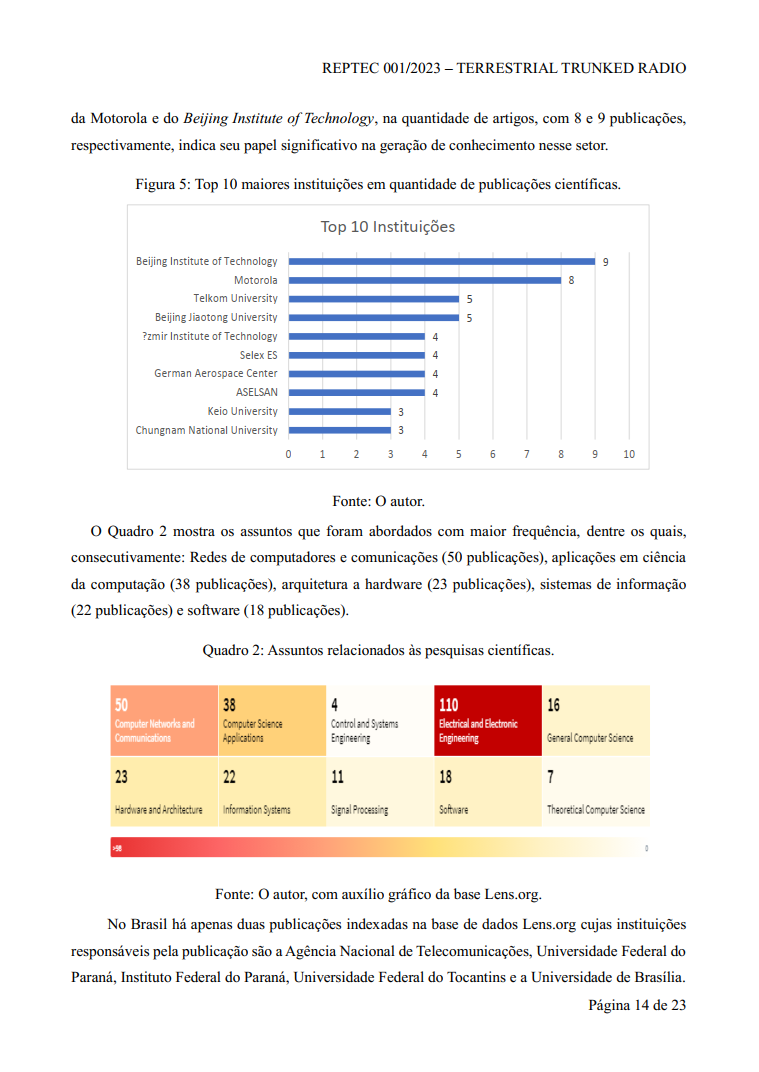
\includegraphics[width=0.8\textwidth]{img/Relatorio_1.png}
    \caption{Resultado da Análise de Dados em um Relatório - Gráficos}
    \label{fig:relatorio 1}
\end{figure}

\begin{figure}[H]
    \centering
    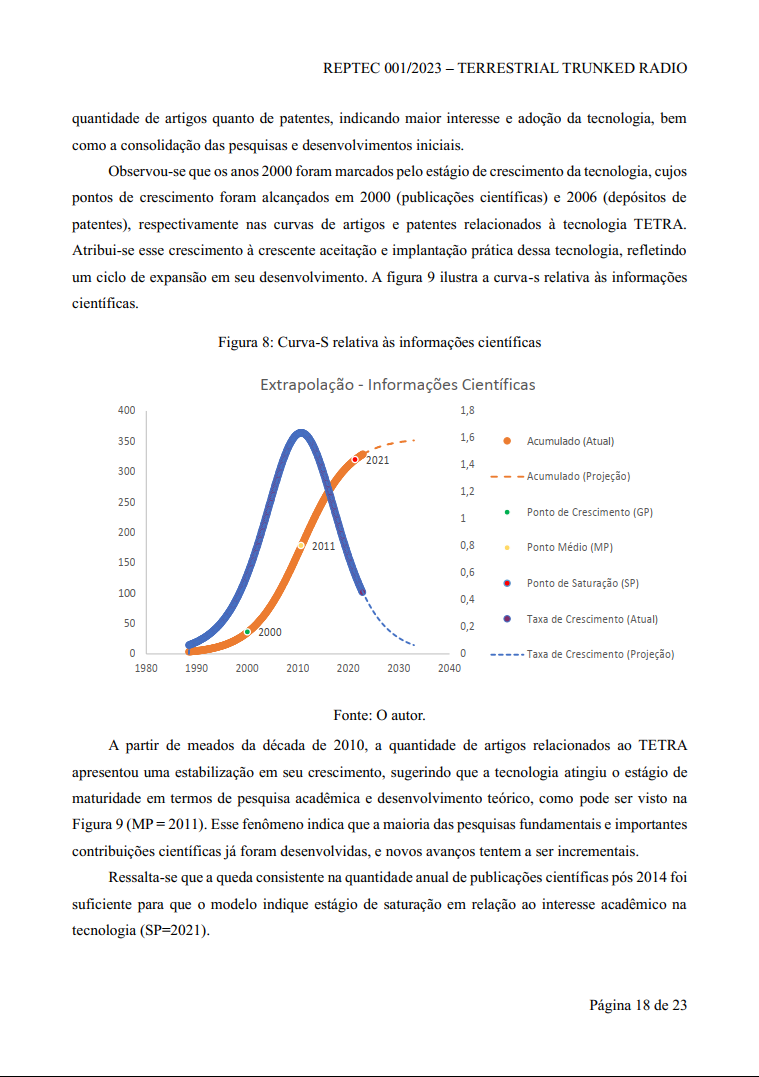
\includegraphics[width=0.8\textwidth]{img/Relatorio_2.png}
    \caption{Resultado da Análise de Dados em um Relatório - Curva S}
    \label{fig:relatorio 2}
\end{figure}

  \subsection{Curva~S de Maturidade Tecnológica}
  \label{sec:curva-s}

  A curva~S é um modelo gráfico que descreve o ciclo de vida de uma tecnologia
ao longo do tempo, relacionando o acúmulo de patentes ou publicações científicas
com o grau de maturidade tecnológica \cite{foster1986}. Segundo Foster, toda
tecnologia possui limites naturais de desempenho, e à medida em que esses limites
são aproximados, o esforço necessário para obter novos avanços cresce
exponencialmente --- ao passo que uma nova tecnologia concorrente pode emergir
a partir de um novo patamar de desempenho, iniciando sua própria curva~S
\cite{foster1986}. Esse fenômeno de descontinuidade tecnológica é fundamental
para a compreensão da dinâmica de substituição entre tecnologias e para a
orientação estratégica de investimentos em PD\&I.

\begin{figure}[H]
    \centering
    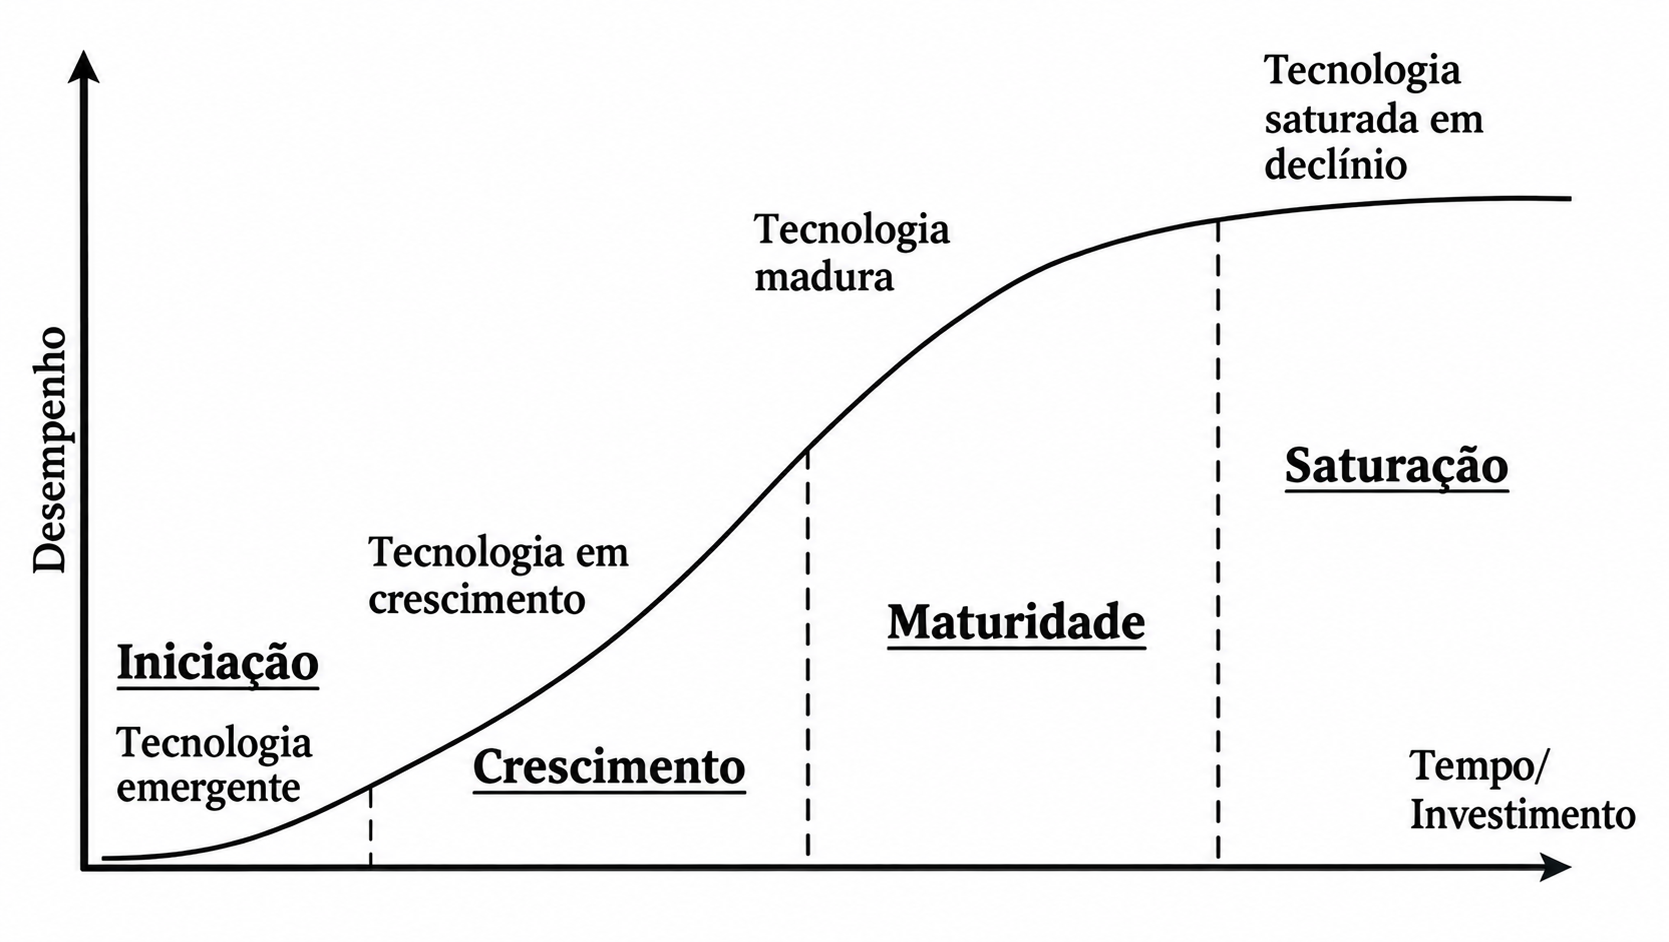
\includegraphics[width=0.7\textwidth]{img/S_Curve_Madeo.png}
    \caption{Curva S \cite{madeo2019}}
    \label{fig:s-curve-madeo}
\end{figure}

  O fundamento matemático mais difundido para a curva~S aplicada à substituição
tecnológica é o modelo de Fisher e Pry \cite{fisherpry1971}, que descreve a
fração de substituição de uma tecnologia antiga por uma nova como uma função
logística do tempo. Ernst \cite{ernst1997} aplicou esse raciocínio à contagem
\emph{acumulada} de depósitos de patentes ao longo do tempo, propondo que o
ciclo de vida de uma tecnologia, e não apenas a substituição de uma tecnologia
por outra, pode ser descrito por quatro estágios sucessivos:

  \begin{enumerate}[label=(\roman*)]
    \item \textbf{Emergente ou Iniciação}: caracterizada por baixo volume de resultados e
    crescimento inicial lento, típica de tecnologias recentemente introduzidas
    que ainda não atraíram atenção ampla da comunidade científica ou industrial.

    \item \textbf{Crescimento}: marcada por expansão acelerada da produção
    científica e tecnológica, indicando que a tecnologia está sendo ativamente
    pesquisada e desenvolvida por um número crescente de atores.

    \item \textbf{Maturidade}: correspondente à estabilização do crescimento,
    quando a tecnologia alcança um patamar de desenvolvimento consolidado e
    a taxa de novas publicações ou patentes se estabiliza.

    \item \textbf{Declínio ou Saturação}: associada à obsolescência ou à substituição da
    tecnologia por soluções mais avançadas, refletindo uma redução no interesse
    e na produção científica e tecnológica \cite{foster1986}.
  \end{enumerate}

  Rogers \cite{rogers2003} complementa essa perspectiva ao descrever como as
inovações se difundem ao longo do tempo em uma população de adotantes, seguindo
igualmente um padrão em curva~S, o que reforça a robustez do modelo logístico
como ferramenta de leitura de maturidade em domínios distintos (adoção de
inovações, substituição tecnológica, difusão bibliométrica). Kucharavy e De
Guio \cite{kucharavy2011} revisam justamente essa recorrência do padrão em
curva~S em campos tão diversos quanto epidemiologia, demografia e previsão
tecnológica, reforçando que a escolha do modelo logístico para leitura de
maturidade, adotada neste trabalho, não é uma particularidade do domínio de
patentes e publicações científicas, mas uma aplicação de um padrão
matemático amplamente validado.

  \subsubsection{Distinção entre fase de maturidade (curva~S) e \textit{Technology Readiness Level} (TRL)}

  É importante não confundir a fase de maturidade tecnológica descrita nesta
seção com o \textit{Technology Readiness Level} (TRL), uma escala amplamente
utilizada em engenharia de sistemas e gestão de programas de defesa e espaço.
O TRL foi originalmente concebido pela NASA na década de 1970 e formalizado por
Mankins \cite{mankins1995} em nove níveis, do TRL~1 (princípios básicos
observados) ao TRL~9 (sistema real comprovado em ambiente operacional). Trata-se
de uma métrica de prontidão de engenharia, avaliada por critérios técnicos
objetivos (ou por julgamento de especialistas) para \emph{uma solução ou
protótipo específico}, tipicamente no contexto de um único projeto de
desenvolvimento.

  A fase de maturidade obtida pela curva~S, por outro lado, não avalia um
protótipo específico, mas o estágio coletivo de uma \emph{área tecnológica como
um todo}, inferido estatisticamente a partir do volume acumulado de patentes e
publicações científicas ao longo do tempo em toda uma comunidade de
pesquisadores e empresas. Enquanto o TRL responde à pergunta "o quão pronta
está \emph{esta} solução para ser empregada?", a curva~S responde a "em que
estágio de seu ciclo de vida coletivo se encontra \emph{este campo}
tecnológico, considerando o esforço de P\&D mundial documentado em patentes e
artigos?". São, portanto, instrumentos complementares, não substitutos: uma
tecnologia em estágio de "crescimento" na curva~S pode conter, simultaneamente,
soluções específicas em TRLs bastante distintos, e o sistema desenvolvido neste
trabalho não realiza e nem se propõe a realizar avaliação de TRL.

  \subsubsection{Formalização matemática e pontos de leitura (GP, MP, SP)}

  O ajuste de curva~S implementado no sistema é feito sobre a contagem
\emph{cumulativa} de documentos por ano (anos sem publicação são reindexados
como zero antes da soma acumulada, e o ano corrente, ainda incompleto, é
descartado, já que sua contagem parcial seria lida pelo ajuste como uma queda
artificial), por meio da função logística clássica:

$$N(t) = \frac{K}{1 + e^{-r \cdot (t - t_0)}}$$

  onde $N(t)$ é a quantidade acumulada de documentos até o ano $t$; $K$ é a
capacidade máxima ou platô de saturação (assíntota superior, correspondente ao
total estimado de documentos quando a tecnologia amadurecer completamente);
$r$ é a taxa de crescimento, associada à inclinação da subida da curva; e
$t_0$ é o ponto de inflexão --- o ano em que a taxa de publicação é máxima e
$N(t) = K/2$. O ajuste desses três parâmetros aos dados observados é realizado
por regressão não linear, com estimativa
inicial de $K$ como 1,5 vez o valor acumulado mais recente, e a taxa de
crescimento instantânea é obtida por diferenciação numérica sobre a curva
ajustada.

  A partir de $K$, $r$ e $t_0$ já ajustados, o sistema inverte algebricamente
a função logística para obter três pontos de leitura do ciclo de vida --- Ponto
de Crescimento (GP), Ponto Médio (MP) e Ponto de Saturação (SP) --- que
correspondem, exatamente, aos marcos empregados na prática de prospecção
tecnológica da AGITEC, como demonstrado com dados reais de patentes e
publicações sobre a tecnologia TETRA em \cite{reptec2023tetra}, onde as curvas
de extrapolação científica e tecnológica trazem GP, MP e SP anotados
diretamente sobre o gráfico. A inversão é dada por:

$$t = t_0 - \frac{\ln\left(\dfrac{1}{f} - 1\right)}{r}, \qquad f = \frac{N(t)}{K}$$

  A Tabela~\ref{tab:gpmpsp} resume a definição de cada ponto e a fração de $K$
usada como referência padrão, ambas configuráveis por parâmetro:

\begin{table}[H]
\centering
\caption{Pontos de leitura do ciclo de vida tecnológico via curva~S}
\label{tab:gpmpsp}
\begin{tabular}{
  >{\raggedright\arraybackslash}p{2.6cm}
  >{\raggedright\arraybackslash}p{9.2cm}
  >{\centering\arraybackslash}p{2.3cm}
}
\toprule
\textbf{Ponto} & \textbf{Definição} & \textbf{Fração de $K$ (padrão)} \\
\midrule
GP & Ano em que a curva acumulada atinge a fração
\texttt{growth\_}\allowbreak\texttt{threshold} de $K$; antes disso, a tecnologia está em fase
embrionária & 0,10 \\\\
MP & O próprio $t_0$; ano de inflexão, com taxa de publicação
anual máxima & 0,50 (sempre igual a $t_0$) \\\\
SP & Ano em que a curva acumulada atinge a fração
\texttt{saturation\_}\allowbreak\texttt{threshold} de $K$; a partir daí, fase de maturidade &
0,90 \\
\bottomrule
\end{tabular}
\end{table}

  Quando o ano calculado para GP, MP ou SP é posterior ao último ano
efetivamente observado nos dados, ele constitui uma \textbf{projeção}, isto é, uma
extrapolação do ajuste logístico, e não um valor observado, distinção que
o sistema mantém explícita na resposta gerada, seguindo a mesma convenção
visual adotada em \cite{reptec2023tetra} (linha contínua para o acumulado
real, linha tracejada para a projeção).

  \subsubsection{Diagnóstico de confiabilidade do ajuste}

  Um ajuste de curva logística pode convergir numericamente e, ainda assim, ser
pouco confiável, como por exemplo, quando poucos anos de dado levam a um platô
"inventado" por sobreajuste (\textit{overfitting}). Por isso, o sistema também
calcula um coeficiente de determinação $R^2$ sobre os resíduos entre a curva
ajustada e a série acumulada real,

$$R^2 = 1 - \frac{SS_{res}}{SS_{tot}},$$

  e marca o ajuste como não confiável quando: (i) $R^2 < 0{,}90$; (ii) a
saturação atual já ultrapassa 85\% de $K$ com menos de cinco anos de dado
observado (sinal típico de sobreajuste); (iii) a taxa de crescimento $r$ é
nula ou negativa (sem sentido físico para uma curva de acumulação); ou
(iv) $r > 5{,}0$, o que produziria uma curva próxima de um degrau, implausível
para fenômenos de difusão tecnológica. Esse diagnóstico é o que garante que o
GP/MP/SP apresentado ao usuário venha acompanhado de uma indicação clara de
quão bem-fundamentada é a leitura, em vez de apresentar um número sem contexto
de sua incerteza estatística.

\begin{figure}[H]
    \centering
    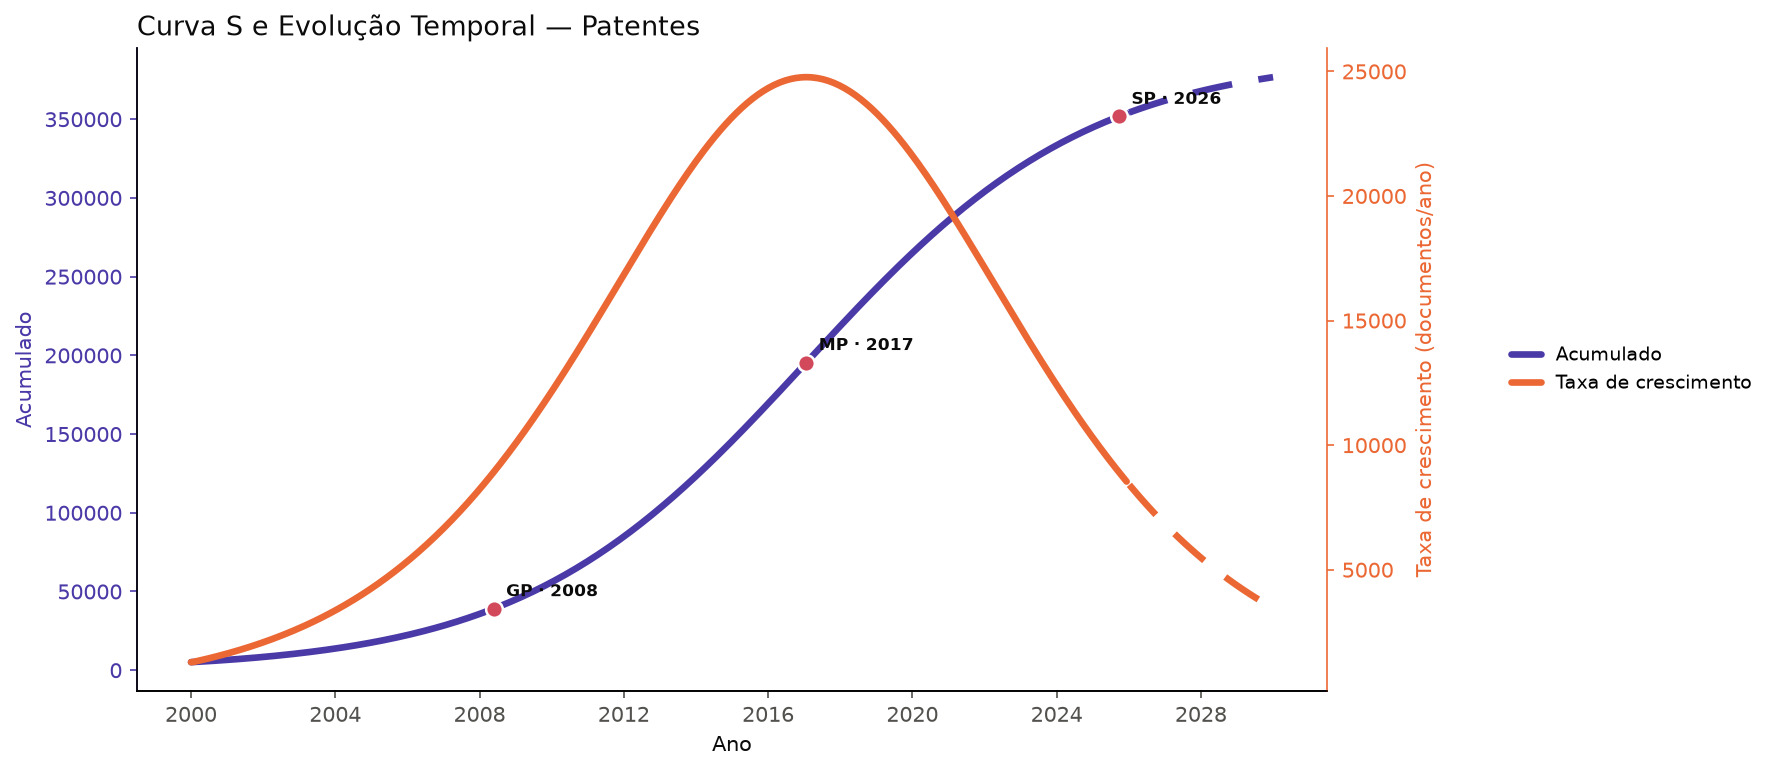
\includegraphics[width=1\textwidth]{img/curva_s_sintetica_gpmpsp.png}
    \caption{Curva~S sintética anotada com os parâmetros $K$, $t_0$ e os pontos de leitura GP, MP e SP. Fonte: elaborado pelo autor.}
    \label{fig:curva-s-sintetica}
\end{figure}

  \subsubsection{Estimação de completude amostral e estabilidade de \textit{ranking}}
  \label{sec:chao1bootstrap}

  Um limite inerente a qualquer indicador construído sobre uma amostra de
patentes ou artigos, incluindo os próprios GP/MP/SP, é que ele reflete o
que foi \emph{recuperado} pela busca, não necessariamente o universo completo
do que existe. Duas técnicas estatísticas complementares, implementadas no
sistema como um módulo de inferência estatística sobre a busca final,
endereçam esse limite sob ângulos distintos.

  O \textbf{estimador Chao1} \cite{chao1984} é uma técnica originária da ecologia de
populações, empregada para estimar a riqueza total de espécies em uma
comunidade a partir de uma amostra incompleta, e que pode ser adaptada ao
contexto bibliométrico tratando cada depositante, instituição ou classificação
tecnológica distinta como uma "espécie" observada. A formulação clássica é

$$
\hat{S}_{Chao1} = S_{obs} + \frac{f_1^2}{2 f_2},
$$

  onde $S_{obs}$ é o número de entidades distintas efetivamente observadas na
amostra, $f_1$ é o número de entidades observadas exatamente uma vez
(\textit{singletons}) e $f_2$ é o número de entidades observadas exatamente
duas vezes (\textit{doubletons}). Quanto mais próxima a razão $S_{obs} /
\hat{S}_{Chao1}$ estiver de 1, mais "saturada" está a amostra, ou seja, mais
próxima de já ter capturado a diversidade real de entidades existentes no
universo pesquisado, e menor a chance de que um aumento no volume de busca
revele muitas entidades novas e relevantes ainda não observadas. Como a
formulação clássica não é definida quando $f_2 = 0$, o sistema emprega a
variante com correção de viés \cite{chao1984},

$$
\hat{S}_{Chao1} = S_{obs} + \frac{f_1 (f_1 - 1)}{2 (f_2 + 1)},
$$

  e considera a amostra \textbf{insuficiente} quando qualquer um de três sinais
é observado: saturação $S_{obs}/\hat{S}_{Chao1} < 0{,}5$; mais de 70\% das
entidades observadas são \textit{singletons} ($f_1 / S_{obs} > 0{,}7$); ou
menos de cinco \textit{doubletons} ($f_2 < 5$), situação em que a própria
estimativa se torna instável.

  O \textbf{método de \textit{bootstrap}} \cite{efron1979} complementa essa leitura verificando
a \textbf{estabilidade} de um indicador derivado da
amostra, como o \textit{ranking} dos dez principais depositantes ou dos dez
principais CPCs. A técnica consiste em reamostrar os documentos observados,
com reposição, um grande número de vezes, recalculando o indicador de
interesse (por exemplo, a composição do \textit{top}-10) a cada reamostragem;
a variância da composição e da ordem do \textit{top}-10 entre as reamostragens
é então usada como medida de confiança --- um \textit{ranking} que muda
substancialmente entre reamostragens é sinal de que a amostra atual ainda é
pequena demais para sustentar aquele agregado específico com confiança. No
sistema, a reamostragem é feita 1.000 vezes, de forma vetorizada, sobre a
distribuição observada de contagens (reamostragem multinomial com o mesmo
tamanho total da amostra original), e a estabilidade de cada entidade do
\textit{top}-10 original é medida como a fração das reamostragens em que ela
permanece entre as dez primeiras.

  O sistema combina as duas técnicas em um laço iterativo de
enriquecimento: a busca final é repetida, solicitando novas páginas de
resultados às APIs, até que a amostra deixe de ser insuficiente segundo o
critério de Chao1 ou até que se esgote um tempo máximo configurado; ao
final, o resultado agregado é resumido em \textit{rankings} \textit{top}-10
acompanhados da estabilidade de cada item e da relevância semântica de cada
documento ao tema pesquisado. A aplicação conjunta dessas duas técnicas é
especialmente relevante para as agregações de classificação tecnológica
(CPC) e área de estudo --- que, por terem cardinalidade tipicamente baixa
(poucas categorias distintas possíveis), tendem a atingir saturação (Chao1) e
estabilidade de \textit{ranking} (\textit{bootstrap}) com volumes de amostra
relativamente pequenos --- e para as agregações de depositante/instituição,
cuja cardinalidade alta e cauda longa tornam esperável a necessidade de
volumes de busca maiores antes que o \textit{ranking} apresentado possa ser
considerado estatisticamente estável. O objetivo funcional desse módulo é
sinalizar automaticamente ao usuário quando a amostra recuperada ainda é
pequena demais para que o
indicador correspondente seja interpretado com confiança, complementando,
para métricas de \textit{ranking} e diversidade, o mesmo papel que o
diagnóstico de $R^2$ (Seção anterior) já cumpre para o ajuste da curva~S.

  \subsection{\textit{Large Language Models} (LLMs)}

  A modelagem de linguagem é uma das principais abordagens para o avanço da
inteligência linguística das máquinas. Antes de discutir os modelos de grande
escala propriamente ditos, cabe situar brevemente o modelo computacional que os
sustenta: as redes neurais artificiais.

Uma rede neural é um modelo composto por
unidades de processamento simples (neurônios artificiais) organizadas em
camadas, em que cada unidade calcula uma combinação linear ponderada de suas
entradas seguida de uma função de ativação não linear; ao empilhar várias
dessas camadas e ajustar os pesos por retropropagação do erro
(\textit{backpropagation}) sobre grandes volumes de dados, a rede aprende a
aproximar funções extremamente complexas, incluindo a distribuição estatística
de sequências de palavras em um idioma \cite{nielsen2015}. É esse mecanismo de
ajuste de pesos por exposição a dados, e não regras gramaticais programadas
manualmente, que permite aos modelos de linguagem generalizar para textos
nunca vistos durante o treinamento.

  Em geral, busca-se modelar a probabilidade
generativa de sequências de palavras, de modo a prever a ocorrência de
\textit{tokens} futuros dado um contexto \cite{zhao2023}. Os \textit{Large Language
Models} (LLMs) são modelos de linguagem de grande escala baseados na arquitetura
\textit{Transformer} \cite{vaswani2017}, capazes de compreender e gerar texto em
linguagem natural com alta coerência e relevância contextual. Seu treinamento em
extensos \textit{corpora} de texto permite sua aplicação em tarefas diversas, como geração
de resumos, extração de informações, construção de \textit{queries} de busca e
redação de relatórios técnicos.

  A arquitetura \textit{Transformer}, introduzida por Vaswani et al.\ \cite{vaswani2017},
revolucionou o campo do Processamento de Linguagem Natural ao substituir as redes
neurais recorrentes por mecanismos de atenção (\textit{self-attention}), que
permitem ao modelo processar todas as posições de uma sequência simultaneamente,
em vez de sequencialmente, capturando dependências de longo alcance com maior eficiência. Em termos
simplificados, o mecanismo de \textit{self-attention} calcula, para cada palavra
da sequência, um conjunto de pesos que indicam o quanto as demais palavras do
mesmo texto devem influenciar sua representação. Por exemplo, ao processar a
palavra "ela" em uma frase, o mecanismo aprende a atribuir maior peso à palavra
que "ela" retoma anteriormente no texto. Esses pesos são calculados a partir de
três projeções aprendidas de cada \textit{token} de entrada (usualmente
denominadas \textit{query}, \textit{key} e \textit{value}), e o resultado é uma
representação de cada palavra que já incorpora o contexto de toda a sentença.
Esse mecanismo é
fundamental para a compreensão do contexto linguístico e semântico, uma vez que
cada posição da sequência passa a carregar informações sobre as demais posições.

\begin{figure}[H]
    \centering
    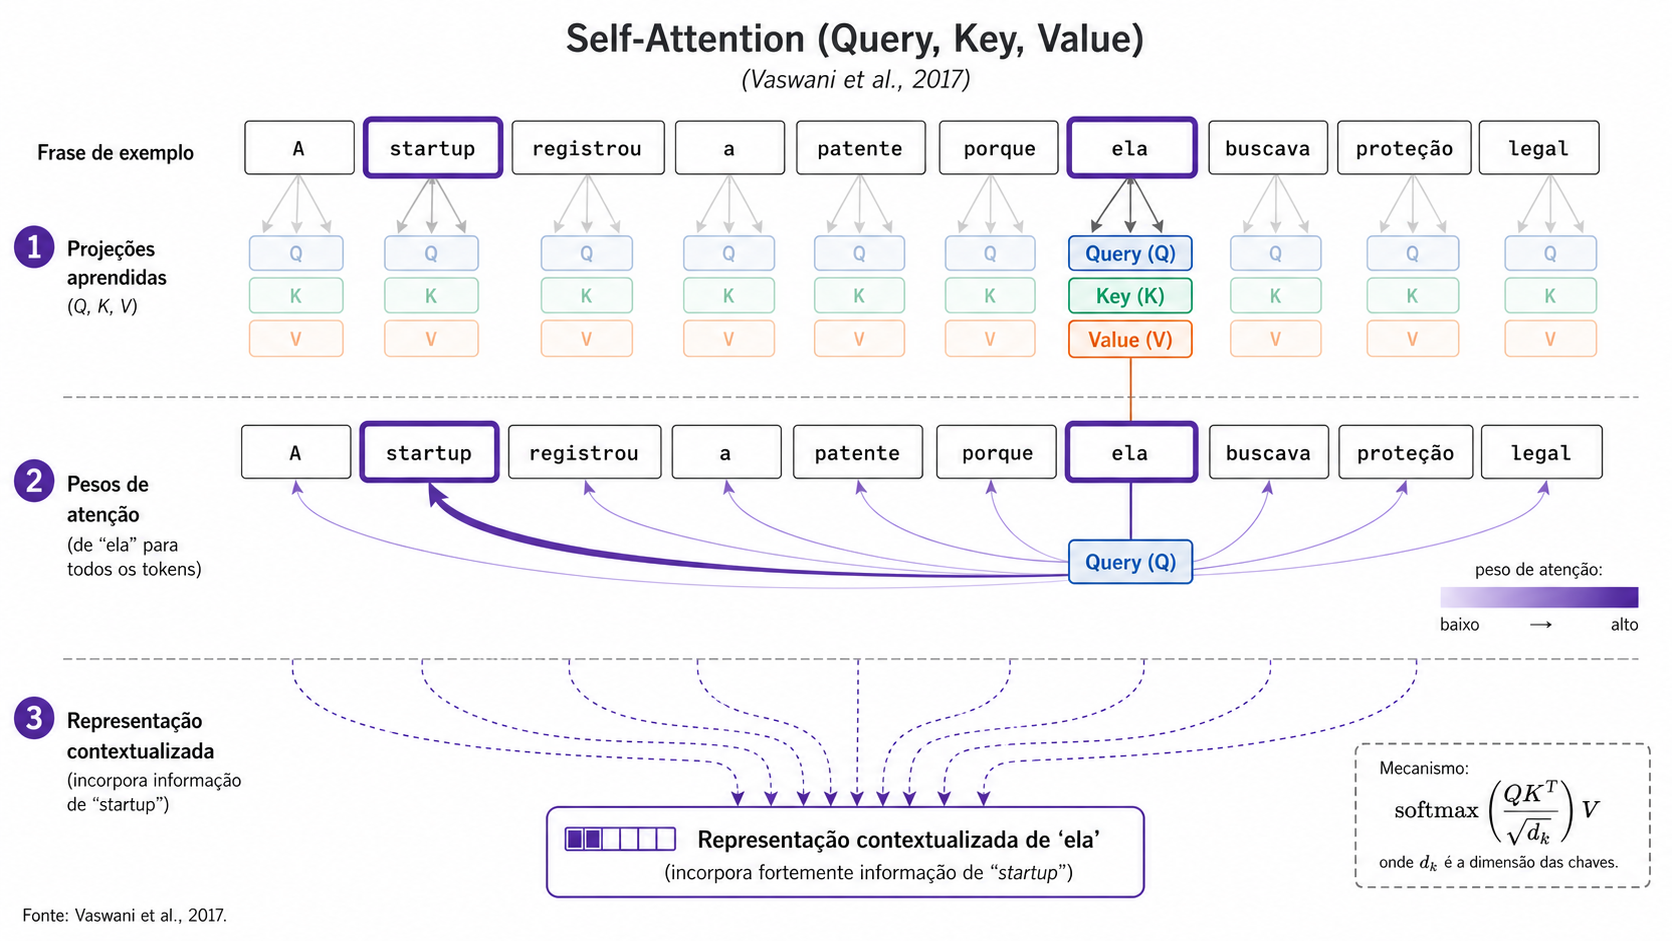
\includegraphics[width=0.95\textwidth]{img/self_attention_transformer.png}
    \caption{Mecanismo de \textit{self-attention} (query/key/value) da arquitetura \textit{Transformer}. Fonte: elaborado pelo autor.}
    \label{fig:self-attention}
\end{figure}

  Diversas famílias de LLMs de propósito geral estão disponíveis atualmente,
cada uma com diferentes compromissos entre custo, desempenho, tamanho e
possibilidade de execução local --- entre elas, GPT (OpenAI), Claude
(Anthropic), Gemini (Google), Qwen (Alibaba) e Gemma (Google), estas duas
últimas disponibilizadas em variantes de menor porte adequadas à execução
local. No sistema desenvolvido, o modelo utilizado não é uma decisão fixa de
arquitetura, mas um parâmetro de configuração substituível, consistente com a
arquitetura hexagonal descrita no Capítulo~3: cada \textbf{ponto de uso} de LLM
--- geração das variações de tema, geração das consultas exploratórias,
geração da consulta final, redação do relatório e revisão linguística do
relatório --- é associado, em tempo de execução, a uma configuração de
provedor e modelo armazenada no banco de dados e editável pela interface
\textit{web}. As etapas de refinamento de tema e de construção de consultas
podem utilizar modelos remotos das famílias \textbf{Claude} (Anthropic) e
\textbf{Gemini} (Google), ou modelos locais; a redação do relatório final via
RAG utiliza um modelo local executado por meio da plataforma Ollama --- nos
testes realizados, os modelos \textbf{Qwen~2.5 (3B-Instruct)} e \textbf{Gemma~3
(4B)} ---, ou, no ambiente institucional, um LLM disponibilizado na intranet
por meio de uma API compatível com o padrão OpenAI.

    \subsubsection{Capacidades e Limitações}

  O aumento da escala dos LLMs tem se mostrado um fator determinante para a
ampliação de suas capacidades. Brown et al.\ \cite{brown2020} demonstraram que
modelos de grande escala são capazes de realizar tarefas a partir de poucos
exemplos fornecidos no próprio \textit{prompt} (\textit{few-shot learning}),
sem necessidade de re-treinamento específico para cada tarefa. Entretanto, os
LLMs apresentam limitações documentadas que precisam ser consideradas em
projetos de aplicação prática:

  \textbf{Alucinações}: os LLMs podem gerar conteúdo que parece plausível, mas
é factualmente incorreto \cite{ji2022}. Esse fenômeno ocorre porque o modelo
produz texto com base em padrões estatísticos aprendidos durante o treinamento,
e não por raciocínio sobre fatos verificáveis. Ji et al.\ \cite{ji2022}
apresentam uma revisão sistemática sobre a ocorrência e mitigação de alucinações
em sistemas de geração de linguagem natural, destacando que esse é um dos
principais desafios para a adoção de LLMs em aplicações críticas. Em tarefas
onde a precisão factual é essencial, como na geração de relatórios técnicos
de prospecção, as alucinações representam um risco significativo que deve
ser mitigado por mecanismos complementares, como o RAG e a validação humana.

  \textbf{Limitações de contexto}: cada LLM possui um limite máximo de
\textit{tokens} que podem ser processados em uma única chamada \cite{zhao2023}.
Isso impõe restrições ao volume de documentos que podem ser incluídos no
contexto de uma requisição, exigindo estratégias de segmentação e seleção dos
trechos mais relevantes.

  \textbf{Custo e dependência de infraestrutura}: LLMs remotos disponibilizados
via API apresentam custo recorrente por \textit{token} consumido \cite{brown2020}.
Em aplicações com alto volume de requisições ou grandes quantidades de texto,
esses custos podem se tornar proibitivos. Além disso, o uso de modelos externos
implica dependência de conectividade e de disponibilidade do serviço, além de
possíveis restrições ao processamento de dados sensíveis.

  \textbf{Modelos locais}: a execução local de LLMs, por meio de plataformas
como o Ollama, elimina os custos recorrentes e garante a privacidade dos dados,
porém exige capacidade computacional adequada \cite{zhao2023}. Modelos locais de
menor porte, como o Qwen~2.5 (3B-Instruct) e o Gemma~3 (4B), testados neste projeto, apresentam
desempenho aceitável em máquinas comuns, mas com tempo de inferência superior ao
de modelos remotos e com possível redução na qualidade da geração de texto,
especialmente em tarefas que exigem raciocínio complexo ou geração de português
formal de alta qualidade. Na prática do projeto, a limitação mais recorrente
observada nesses modelos foi a concordância verbal com sujeito distante (por
exemplo, "a concentração de depositantes \ldots\ indicam"), o que motivou a
etapa de revisão linguística assistida descrita na Seção~\ref{sec:fase5}.

  \subsection{Engenharia de \textit{Prompt}}

  A engenharia de \textit{prompt} (\textit{prompt engineering}) refere-se ao
conjunto de técnicas e estratégias utilizadas para formular as instruções
enviadas a um LLM de modo a maximizar a qualidade e a adequação das respostas
geradas \cite{white2023}. Dado que o comportamento de um LLM é altamente
sensível à formulação das instruções recebidas, a definição cuidadosa dos
\textit{prompts} representa uma etapa crítica no desenvolvimento de sistemas
baseados em IA generativa e, no sistema aqui descrito, essa etapa não se
restringe a um único ponto do fluxo: praticamente toda interação com um LLM
remoto (refinamento de tema, geração de consultas exploratórias, geração das
variantes de consulta final) é mediada por um \textit{prompt} de sistema
cuidadosamente estruturado, o que faz da engenharia de \textit{prompt} um
componente estrutural do projeto, e não um detalhe de implementação.

  White et al.\ \cite{white2023} descrevem um catálogo de padrões de
\textit{prompt engineering} aplicáveis a diferentes contextos de uso de LLMs,
incluindo padrões para definição de papel (\textit{persona pattern}), para
estruturação da saída esperada e para restrição do comportamento do modelo.
Dentre as técnicas mais relevantes para o presente projeto destacam-se: a
definição explícita do papel do modelo por meio de um \textit{system prompt},
que orienta o LLM sobre o contexto em que deve operar e as restrições que deve
observar; o encadeamento de raciocínio (\textit{chain-of-thought}), que
induz o modelo a explicitar etapas intermediárias antes de produzir a resposta
final, melhorando o desempenho em tarefas que exigem raciocínio estruturado
\cite{wei2022}; e o uso de exemplos contrastantes (\textit{few-shot learning}),
em que pares de exemplo bom/ruim são fornecidos no próprio \textit{prompt} para
forçar diversidade e especificidade reais nas respostas geradas, em vez de
paráfrases superficiais.

  Wei et al.\ \cite{wei2022} demonstraram empiricamente que a técnica de
\textit{chain-of-thought prompting} --- na qual alguns exemplos de raciocínio
passo a passo são fornecidos no \textit{prompt} --- melhora significativamente
o desempenho de LLMs de grande escala em tarefas de raciocínio aritmético,
de senso comum e simbólico, especialmente em modelos com mais de 100 bilhões
de parâmetros. No sistema desenvolvido, essa técnica é aplicada de forma
particularmente disciplinada nas instruções de geração de consultas: o
\textit{prompt} de sistema explicita uma sequência numerada de passos de
raciocínio (identificação de conceitos semânticos, seleção de conceitos
centrais versus secundários, montagem de grupos de termos) que o modelo deve
seguir antes de produzir a consulta final.

  Um padrão adicional, não descrito no catálogo original de White et al.\
\cite{white2023}, mas empregado de forma sistemática no sistema desenvolvido, é
o que pode ser chamado de \textbf{autocorreção por métrica determinística}: a
saída do LLM (uma consulta booleana) é avaliada por um componente de código
determinístico --- não pela própria LLM se autoavaliando --- que calcula um
escore objetivo de complexidade estrutural da consulta; caso esse escore
ultrapasse um limiar configurável, o resultado exato da avaliação (quantidade
de operadores, profundidade de aninhamento, número de termos) é reinjetado no
\textit{prompt} da tentativa seguinte, em um sufixo de simplificação que cita
de volta os números da tentativa anterior. Após um número máximo de tentativas
(tipicamente três), o sistema não falha: retorna a tentativa menos complexa das
geradas, com um aviso explícito ao usuário. Esse mecanismo evidencia um limite
prático da engenharia de \textit{prompt} isolada -- instruções textuais nem
sempre são suficientes para restringir o comportamento do modelo de forma
confiável --- e a necessidade de complementá-la com verificação programática
externa ao próprio LLM.

    \subsubsection{Função de Complexidade de Consulta}
    \label{sec:complexidade}

  A métrica de complexidade citada acima não é derivada de nenhuma referência
bibliográfica externa: trata-se de uma \textbf{função heurística concebida
pelos próprios autores deste trabalho}, motivada empiricamente pelo
comportamento observado das APIs consultadas. Ao longo do desenvolvimento,
constatou-se repetidas vezes que consultas booleanas mais "abrangentes", com
muitos termos e muitos operadores \texttt{OR}/\texttt{AND} aninhados, não
produziam necessariamente mais resultados, mas sim erros ou zero resultados: a
a API do OPS retorna erro de servidor
quando, por exemplo, vários \texttt{OR} são utilizados, ao invés de retonar mais resultados, o que seria o logicamente esperado. Diante da ausência de um limite de complexidade
publicado pelas próprias APIs, optou-se por desenvolver uma métrica interna
que servisse de \textit{guardrail} preventivo, calculada e verificada
\emph{antes} de qualquer consulta ser efetivamente enviada a uma API externa.

  A função combina quatro sub-escores independentes, cada um normalizado no
intervalo $[0, 100]$ contra uma base de referência escolhida empiricamente, e
combinados por uma média ponderada:

$$
\begin{aligned}
\text{operator\_score} &= \min\left(100,\; \frac{n_{\text{operadores}}}{10} \times 100\right) \\[4pt]
\text{nesting\_score} &= \min\left(100,\; \frac{d_{\text{aninhamento}}}{5} \times 100\right) \\[4pt]
\text{term\_score} &= \min\left(100,\; \frac{n_{\text{termos}}}{20} \times 100\right) \\[4pt]
\text{length\_score} &= \min\left(100,\; \frac{c_{\text{caracteres}}}{1000} \times 100\right)
\end{aligned}
$$

$$
\text{score} = 0{,}2 \cdot \text{operator\_score} + 0{,}3 \cdot \text{nesting\_score} + 0{,}3 \cdot \text{term\_score} + 0{,}2 \cdot \text{length\_score}
$$

  onde $n_{\text{operadores}}$ é a contagem total de ocorrências de
\texttt{AND}/\texttt{OR}/\texttt{NOT} na consulta (por expressão regular,
insensível a maiúsculas/minúsculas); $d_{\text{aninhamento}}$ é a profundidade
máxima de parênteses aninhados --- com um cuidado deliberado no cálculo: um
parêntese de abertura não é contado como um novo nível se o caractere
não-espaço imediatamente anterior também for um parêntese de abertura, já que
os construtores de consulta (Seção~4.2) embrulham mecanicamente cada cláusula
em seus próprios parênteses, o que empilharia parênteses sem representar
aninhamento lógico real caso não houvesse essa correção; $n_{\text{termos}}$ é
a contagem de termos entre aspas; e $c_{\text{caracteres}}$ é o comprimento
bruto, em caracteres, da consulta. Os pesos ($0{,}2$; $0{,}3$; $0{,}3$;
$0{,}2$) e as quatro bases de normalização (10 operadores, 5 níveis de
aninhamento, 20 termos, 1000 caracteres) foram calibrados empiricamente pelos
autores a partir da observação de consultas que efetivamente falhavam nas APIs
consultadas, e não a partir de nenhum estudo ou norma publicada. A partir do
escore final, a consulta é classificada em um de quatro níveis, apresentados
na Tabela~\ref{tab:complexidade}.

\begin{table}[H]
\centering
\caption{Níveis de classificação da função de complexidade de consulta}
\label{tab:complexidade}
\begin{tabular}{lc}
\toprule
\textbf{Nível} & \textbf{Faixa de escore} \\
\midrule
Simples & escore $< 25$ \\
Moderado & $25 \leq$ escore $< 50$ \\
Complexo & $50 \leq$ escore $< 75$ \\
Muito Complexo & escore $\geq 75$ \\
\bottomrule
\end{tabular}
\end{table}

  Como exemplo de aplicação da fórmula, considere uma consulta hipotética com
$n_{\text{operadores}} = 6$, $d_{\text{aninhamento}} = 3$, $n_{\text{termos}} =
9$ e $c_{\text{caracteres}} = 420$. Os sub-escores resultantes são:

$$
\text{operator\_score} = \min\left(100,\; \frac{6}{10}\times 100\right) = 60
$$
$$
\text{nesting\_score} = \min\left(100,\; \frac{3}{5}\times 100\right) = 60
$$
$$
\text{term\_score} = \min\left(100,\; \frac{9}{20}\times 100\right) = 45
$$
$$
\text{length\_score} = \min\left(100,\; \frac{420}{1000}\times 100\right) = 42
$$

  e o escore final é

$$
\text{score} = 0{,}2(60) + 0{,}3(60) + 0{,}3(45) + 0{,}2(42) = 12 + 18 + 13{,}5 + 8{,}4 = 51{,}9,
$$

  classificando essa consulta hipotética como \textbf{Complexa} (Tabela~\ref{tab:complexidade}), abaixo, portanto, do limiar padrão de $60$ pontos
adotado como corte de aceitação, ou seja, ainda dentro do limite, mas
próxima o suficiente dele para que, em uma consulta real com poucos termos ou
operadores a mais, o sistema já acionasse o ciclo de retentativa com
simplificação assistida.

  Além do escore em si, a função também emite avisos textuais complementares, como por exemplo, mais de 15 operadores no total, aninhamento acima de 4 níveis,
parênteses desbalanceados, mais de 5 termos repetidos, comprimento acima de
2000 caracteres, ou contagem de operadores \texttt{OR} mais que o dobro da
contagem de \texttt{AND}; e recomendações textuais de simplificação
(reduzir termos para cerca de 5 a 8, limitar aninhamento, remover duplicatas),
usadas tanto na interface do usuário quanto no sufixo de simplificação
reinjetado no \textit{prompt} da LLM descrito no início desta seção.

    \subsubsection{Validação e correção de saída estruturada}
    \label{sec:defesa-camadas}

  A função de complexidade de consulta (Seção~\ref{sec:complexidade}) resolve
o problema de uma consulta \emph{sintaticamente válida}, mas
\emph{estruturalmente arriscada} para as APIs externas. Um problema anterior e
distinto, comum a qualquer sistema que dependa de um LLM para produzir dados
estruturados (aqui, objetos JSON representando termos, campos e operadores de
consulta), é o de a própria saída do modelo não ser sequer um JSON válido, ou
não respeitar o formato esperado, já que, tecnicamente, um LLM gera texto,
não estruturas de dados, e sua aderência a um formato solicitado depende
inteiramente de quão bem o modelo segue a instrução. O sistema desenvolvido
resolve esse problema com uma defesa organizada em camadas sucessivas, cada
uma cobrindo os casos que a anterior deixa passar:

  \begin{enumerate}[label=(\alph*)]
    \item \textbf{Modo JSON nativo}, quando disponível: para o provedor
    Gemini, a chamada é configurada para exigir explicitamente que a resposta
    seja um JSON sintaticamente válido, o que reduz substancialmente a
    ocorrência de erros de formatação já na origem. O provedor Anthropic, no
    momento da implementação, não expõe esse mesmo mecanismo de imposição de
    formato para o caso de uso do sistema, de modo que sua saída depende
    apenas de instrução textual explícita no \textit{prompt} ("retorne
    apenas JSON válido") e de extração posterior de blocos de código ou
    interpretação direta da resposta como JSON.
    \item \textbf{Reparo sintático leve}, por expressão regular, que remove
    vírgulas finais indevidas e insere vírgulas ausentes entre membros de um
    objeto ou lista antes de uma nova tentativa de interpretação do texto como
    JSON --- erros comuns, sobretudo em modelos locais de menor porte, e de
    baixo risco de correção incorreta. Se, ainda assim, a resposta não puder
    ser interpretada, a chamada ao LLM é repetida, em vez de a etapa falhar na
    primeira resposta malformada.
    \item \textbf{Recuperação tolerante a item individual corrompido}: no
    fluxo de refinamento de tema, quando a resposta é uma lista de
    candidatos e apenas um deles está malformado, o sistema extrai
    individualmente cada objeto da lista (por contagem de profundidade de
    chaves) e descarta apenas o candidato corrompido, em vez de descartar a
    chamada inteira por um único item defeituoso.
    \item \textbf{Validação de esquema}: o JSON já sintaticamente válido é
    então validado contra um esquema de tipos e campos esperados, rejeitando
    qualquer estrutura que não corresponda ao formato de saída definido pelo
    sistema.
    \item \textbf{Validação semântica de conteúdo}: funções específicas
    verificam se cada termo retornado não é uma \textit{stopword} ou palavra
    genérica isolada, se cada grupo de termos respeita a forma esperada
    (operador e lista de termos) e se o operador informado pertence ao
    conjunto permitido (\texttt{AND} ou \texttt{OR}); campos que a LLM
    eventualmente produza fora da lista de campos habilitados para a API em
    uso são removidos nesta etapa.
    \item \textbf{Normalização final}: o objeto validado é remodelado de
    acordo com os campos efetivamente habilitados por configuração,
    zerando qualquer campo não habilitado antes de prosseguir para a
    construção da consulta pelos construtores da Seção~4.2.
  \end{enumerate}

  Assim como a função de complexidade de consulta, essa sequência de camadas
de defesa é uma decisão de engenharia do próprio projeto, não uma técnica
padronizada por nenhuma das referências bibliográficas citadas neste
capítulo, concebida especificamente para lidar com a variabilidade de
aderência a formato observada entre os provedores de LLM utilizados, e
constitui, junto com o RAG (Seção~\ref{sec:rag}) e o ciclo de validação humana
(Capítulo~4), a terceira linha de defesa do sistema contra o risco de
alucinação e de saída inconsistente apontado por Ji et al.\ \cite{ji2022}.

  \subsection{\textit{Retrieval-Augmented Generation} (RAG)}
  \label{sec:rag}

  A técnica de \textit{Retrieval-Augmented Generation} (RAG) foi formalmente
introduzida por Lewis et al.\ \cite{lewis2020} como um modelo que combina
memória paramétrica (o conhecimento codificado nos pesos do modelo durante o
treinamento) com memória não paramétrica (uma fonte de conhecimento externa
acessada por um mecanismo de recuperação). Em vez de depender exclusivamente
do conhecimento parametrizado internamente no LLM, o RAG enriquece o contexto
enviado ao modelo com trechos relevantes recuperados de uma base de documentos
real, reduzindo significativamente a ocorrência de alucinações \cite{ji2022, gao2024}.

  Conceitualmente, o processo RAG pode ser descrito em duas etapas \cite{lewis2020}:
(i) dado um texto de consulta $x$, o sistema recupera um conjunto de documentos
$z = \{z_1, \ldots, z_n\}$ de uma base de conhecimento, utilizando uma função
de similaridade semântica; (ii) a partir de $x$ e dos documentos recuperados $z$,
o modelo gera a resposta $y$. Gao et al.\ \cite{gao2024} propõem uma taxonomia
que classifica as implementações de RAG em três categorias progressivamente mais
sofisticadas:

  \begin{itemize}
    \item \textbf{RAG Naive (ingênuo)}: o padrão mais simples --- indexação de
    documentos, recuperação dos $k$ trechos mais similares à consulta por
    similaridade vetorial, e concatenação direta desses trechos como texto puro
    dentro do \textit{prompt} de usuário enviado ao LLM, sem nenhum
    processamento intermediário sobre os trechos recuperados nem uso de
    \textit{function calling}/\textit{tool use}.
    \item \textbf{RAG Avançado}: adiciona etapas de pré-recuperação (reescrita
    ou expansão da consulta, roteamento entre diferentes bases) e
    pós-recuperação (\textit{reranking} dos trechos recuperados, compressão do
    contexto) em torno do núcleo do RAG Naive.
    \item \textbf{RAG Modular}: reorganiza o processo em módulos independentes
    e recombináveis (por exemplo, módulos de busca híbrida, memória de
    conversas anteriores, ou múltiplas rodadas de recuperação intercaladas com
    geração), permitindo arquiteturas mais flexíveis e adaptadas a tarefas
    específicas.
  \end{itemize}

  O sistema desenvolvido neste trabalho adota uma variante de \textbf{RAG Naive, inteiramente local}, acrescida de dois pós-processamentos leves típicos do RAG Avançado.
O corpus indexado é composto pelo título e pelo resumo de cada patente e de
cada artigo recuperado na busca final da sessão, segmentados em fragmentos,
convertidos em \textit{embeddings} por um modelo executado localmente e
armazenados em um banco de dados vetorial também local (ChromaDB, detalhado
na Seção~\ref{sec:chromadb}), isolados por sessão de pesquisa. No momento da
geração de cada seção do relatório, os fragmentos mais similares à consulta
semântica daquela seção são recuperados e concatenados como \textbf{texto
puro} dentro do \textit{prompt} de usuário enviado ao modelo de linguagem
\textbf{local} --- deliberadamente sem uso de \textit{function
calling}/\textit{tool use}, tanto por simplicidade de integração quanto porque
os modelos locais de menor porte têm suporte mais limitado e menos confiável a
chamadas de ferramentas estruturadas do que os modelos remotos de maior escala.

  Os dois pós-processamentos aplicados sobre os fragmentos recuperados são:
(i) um \textbf{corte relativo de relevância}, que descarta todo fragmento cujo
escore de similaridade seja inferior a uma fração configurável (por padrão,
$0{,}75$) do escore do fragmento mais relevante, eliminando documentos
periféricos ao tema que a simples seleção dos $k$ mais similares traria de
qualquer forma; e (ii) a remoção dos escores de similaridade do texto enviado
ao modelo, que, quando presentes, tendiam a ser reproduzidos literalmente no
relatório. Cada fragmento carrega ainda, em seus metadados, a citação no
formato autor-data e a referência bibliográfica completa no padrão ABNT do
documento de origem, montadas a partir dos metadados estruturados devolvidos
pelas APIs; essas são as únicas citações que o modelo está autorizado a
utilizar no texto (Seção~\ref{sec:fase5}).

  A concepção inicial do sistema previa uma segunda coleção vetorial, com
relatórios de prospecção já elaborados pela AGITEC, indexados como referência
de estrutura e estilo redacional. Essa abordagem foi substituída, na
implementação, por um mecanismo determinístico: a estrutura do relatório é
fixada por um \textit{template} LaTeX que reproduz o padrão REPTEC
\cite{reptec2023tetra}, e as seções cujo texto é essencialmente o mesmo em
todo relatório (Finalidade e Metodologia, por exemplo) são inseridas como
texto fixo, sem passar pelo modelo. Essa escolha elimina, nessas seções, o
risco de alucinação e reduz o volume de contexto de cada chamada, cabendo ao
modelo apenas a redação das seções que efetivamente dependem dos dados da
busca.

Essa escolha de arquitetura é deliberada e alinhada a dois
objetivos que a motivam: manter toda a etapa de geração do relatório final, que é a mais sensível em termos de volume de contexto e, potencialmente, de
sigilo dos dados sob análise, inteiramente dentro da infraestrutura local,
sem envio de dados a serviços remotos; e produzir um relatório que siga
fielmente o padrão REPTEC já estabelecido pela literatura institucional
\cite{agitec2024, reptec2023tetra}, com cada seção fundamentada nos documentos
efetivamente recuperados na busca, mitigando o risco de alucinação factual
apontado por Ji et al.\ \cite{ji2022}.

%% TODO (imagem desatualizada): pipeline_rag_local.png ainda mostra a
%% concepção inicial (duas coleções, nomic-embed-text, Qwen 2.5). Redesenhar
%% com: título+resumo da busca final -> fragmentos -> embeddings SBERT ->
%% ChromaDB (coleção única, filtrada por sessão) -> top-k + corte relativo ->
%% prompt da seção (+ citações permitidas) -> LLM local -> validador de texto.
% \begin{figure}[H]
%     \centering
%     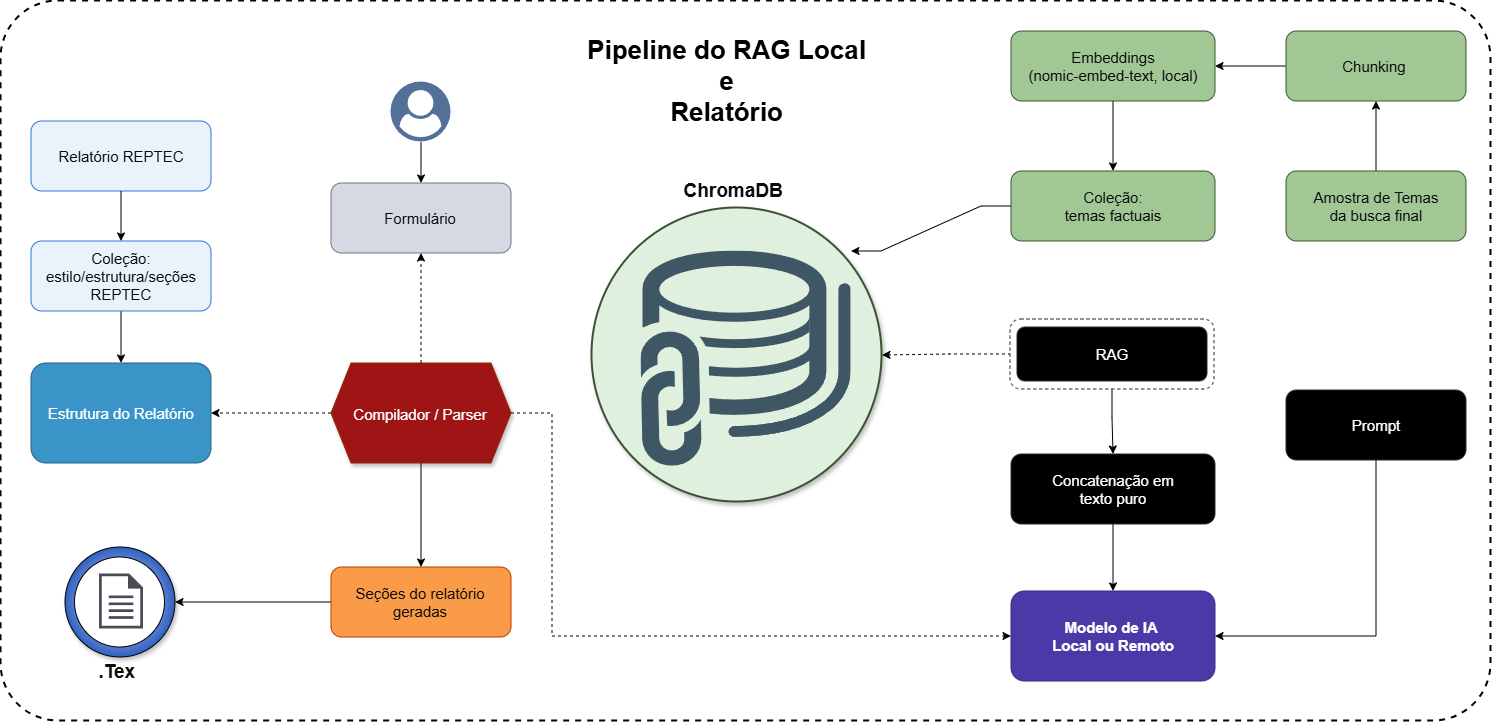
\includegraphics[width=1\textwidth]{img/pipeline_rag_local.png}
%     \caption{Pipeline do RAG local: da coleção indexada no ChromaDB até a seção redigida pelo LLM local. Fonte: elaborado pelo autor.}
%     \label{fig:pipeline-rag-local}
% \end{figure}

  \subsection{\textit{Embeddings} e Bancos de Dados Vetoriais}

  Os \textit{embeddings} são representações vetoriais densas de textos em um
espaço de alta dimensionalidade, obtidas por modelos de linguagem treinados para
capturar a semântica e as relações contextuais entre palavras, frases ou
documentos \cite{mikolov2013}. O trabalho seminal de Mikolov et al.\
\cite{mikolov2013} demonstrou que modelos de representação distribuída de palavras
são capazes de capturar um grande número de relações sintáticas e semânticas
precisas, de modo que textos com significado similar são mapeados para vetores
próximos no espaço vetorial. Isso permite realizar buscas por similaridade
semântica, ou seja, encontrar documentos relevantes para uma consulta sem
depender de correspondência exata de palavras-chave.

  Reimers e Gurevych \cite{reimers2019} introduziram o modelo Sentence-BERT
(SBERT), que estende a arquitetura BERT com redes siamesas e de triplas para
derivar \textit{embeddings} de sentenças semanticamente significativos,
comparáveis por similaridade de cosseno. O SBERT reduziu drasticamente o custo
computacional de tarefas de similaridade semântica, tornando viável a comparação
eficiente de grandes coleções de documentos, fundamento direto do subsistema
de recuperação em sistemas RAG, e também da etapa de pontuação de termos
descrita na Seção~\ref{sec:extracao-termos}.

  No contexto do RAG, os \textit{embeddings} são o mecanismo que permite
conectar uma consulta do usuário aos trechos mais relevantes da base de
documentos indexados \cite{gao2024}. Para cada consulta, o sistema gera um vetor
de representação semântica e compara esse vetor com os vetores dos fragmentos
indexados, selecionando os mais próximos por similaridade de cosseno. O banco de
dados vetorial adotado no sistema desenvolvido é o \textbf{ChromaDB}, cujos
detalhes técnicos de configuração são apresentados na Seção~\ref{sec:chromadb},
junto das demais ferramentas de infraestrutura local.

  \subsection{Filtragem de Documentos por Idioma e por Relevância ao Tema}
  \label{sec:filtragem-documentos}

  Antes que os documentos recuperados por qualquer uma das APIs alimentem as
etapas de extração de termos (Seção~\ref{sec:extracao-termos}) ou de geração
de relatório, dois filtros independentes atuam em nível de documento, reduzindo o conjunto de trabalho aos itens efetivamente úteis.

  O \textbf{filtro de idioma} descarta documentos cujo título e resumo não
sejam identificados com confiança como texto em língua inglesa, idioma
predominante e mais uniformemente disponível nas bases de patentes e artigos
consultadas, por meio de uma biblioteca de detecção estatística de idioma
aplicada sobre o texto concatenado de título e resumo. Esse filtro é
necessário porque nem todos os registros de patente possuem resumo em inglês
disponível (Seção~2.7.1), e um resumo em outro idioma, se não descartado,
distorceria tanto as pontuações de termo (Seção~\ref{sec:extracao-termos})
quanto o embedding do documento usado no filtro de relevância descrito a
seguir.

  O \textbf{filtro de relevância documento-tema} avalia, para cada documento
que passou pelo filtro de idioma, o quão semanticamente próximo ele está do
tema de pesquisa informado pelo usuário. O sistema gera um \textit{embedding}
do tema e um \textit{embedding} de cada documento com uma estratégia de
composição de texto por prioridade de campo (resumo, se disponível e
suficientemente longo; caso contrário, título e resumo combinados; caso
contrário, apenas o título), e calcula a similaridade de cosseno entre os
dois vetores:

$$
\text{sim}(\vec{t}, \vec{d}) = \frac{\vec{t} \cdot \vec{d}}{\lVert \vec{t} \rVert \, \lVert \vec{d} \rVert} \in [-1, 1],
$$

  onde $\vec{t}$ é o \textit{embedding} do tema e $\vec{d}$ é o \textit{embedding}
do documento. Na prática, como os \textit{embeddings} de sentença aqui
empregados (Seção~2.6) tendem a produzir vetores em uma região restrita do
espaço, os valores observados de $\text{sim}(\vec{t}, \vec{d})$ raramente são
negativos, ainda que a faixa teórica da similaridade de cosseno seja
$[-1, 1]$. O documento é marcado como aprovado quando essa similaridade
atinge ou ultrapassa um limiar de $0{,}4$; documentos aprovados e reprovados
são mantidos em listas ordenadas separadamente por escore, de modo que o
critério de corte permaneça auditável. É esse filtro que efetivamente decide quais documentos chegam à etapa de extração
de termos, funcionando como um portão de qualidade a montante de todo o
restante do \textit{pipeline} de análise textual.

  Complementarmente às técnicas de \textit{embedding} descritas na
Seção~2.6, o pipeline de extração de termos do sistema
(Seção~\ref{sec:extracao-termos}) combina técnicas consagradas de
recuperação de informação para gerar, pontuar e ranquear os candidatos a
termo-chave extraídos de título e resumo de cada documento: PatternRank,
BM25F, KeyBERT, \textit{Reciprocal Rank Fusion} (RRF) e C-value.

  O \textbf{PatternRank} \cite{schopf2022} é um método de geração de
candidatos baseado em padrões gramaticais: em vez de fatiar o texto em
janelas de palavras de tamanho fixo, extrai as frases nominais maximais que
obedecem a um padrão de classes gramaticais --- no sistema, zero ou mais
adjetivos seguidos de um ou mais substantivos ---, de modo que cada candidato
já nasce como uma expressão gramaticalmente completa (\textit{"perovskite
solar cell"}), e não como um fragmento arbitrário (\textit{"solar cell
efficiency of"}).

  O \textbf{BM25} \cite{robertson2009} é a função de ranqueamento
probabilístico que se tornou padrão em mecanismos de busca textual, sucessora
direta da ponderação TF-IDF (\textit{Term Frequency--Inverse Document
Frequency}) formalizada por Salton e Buckley \cite{saltonbuckley1988}. Assim
como o TF-IDF, favorece termos frequentes em poucos documentos do conjunto;
diferentemente dele, satura a contribuição da frequência do termo
(parâmetro $k_1$), de modo que a décima ocorrência de um termo acrescente
muito menos que a primeira, e normaliza essa frequência pelo tamanho do
documento (parâmetro $b$), evitando que documentos longos sejam favorecidos
apenas por conterem mais palavras. O \textbf{BM25F} \cite{robertson2004} estende
o BM25 a documentos com múltiplos campos ponderados: título e resumo são
tratados como campos distintos de um mesmo documento, cada um com seu peso,
e as frequências ponderadas são combinadas \emph{antes} da saturação --- e
não somando dois escores BM25 independentes, o que distorceria a saturação.

  O \textbf{KeyBERT} \cite{grootendorst2020}, por sua vez, é uma técnica de
extração de palavras-chave baseada em \textit{embeddings} de sentença
(Seção~2.6): tanto o texto de referência quanto cada candidato a termo são
convertidos em vetores pelo mesmo modelo de \textit{embedding}
\cite{reimers2019}, e o escore do candidato é dado pela similaridade de
cosseno entre os dois vetores --- de modo que, diferentemente do BM25F, que
mede apenas recorrência estatística, o KeyBERT captura proximidade semântica,
inclusive entre um candidato e um sentido que não compartilhe exatamente as
mesmas palavras do texto de referência.

  Como BM25F e KeyBERT produzem escores em escalas incomparáveis (o primeiro
ilimitado, o segundo uma similaridade de cosseno), o sistema não os soma: os
dois canais são combinados pela \textbf{\textit{Reciprocal Rank Fusion}}
(RRF) \cite{cormack2009}, que funde \emph{posições} em vez de escores:

$$
\text{RRF}(t) = \sum_{i} \frac{1}{k + \text{posição}_i(t)},
$$

  onde $\text{posição}_i(t)$ é a posição do candidato $t$ no \textit{ranking}
do canal $i$ e $k = 60$ é a constante de suavização recomendada pelos
autores do método. Um candidato bem posicionado em ambos os canais supera um
candidato excelente em apenas um deles, sem que seja necessário calibrar
pesos entre escalas diferentes. Por fim, o \textbf{C-value}
\cite{frantzi2000} é uma medida de \textit{termhood} para termos compostos,
que penaliza candidatos que ocorrem quase sempre aninhados dentro de um
candidato mais longo (por exemplo, \textit{"ultrafiltration membrane"}
dentro de \textit{"composite ultrafiltration membrane"}), sinalizando
redundância entre termos aninhados. A aplicação dessas técnicas, com os
filtros de fronteira lexical e gramatical aplicados antes e depois da
pontuação, é detalhada passo a passo, com fórmulas e um exemplo numérico, na
Seção~\ref{sec:extracao-termos}, no capítulo da solução proposta.

  \subsection{APIs Utilizadas}

    \subsubsection{OPS --- \textit{Open Patent Services}}

    O \textit{Open Patent Services} (OPS) é uma API REST disponibilizada
pelo Escritório Europeu de Patentes (EPO) que permite acesso programático à base
Espacenet, uma das maiores coleções mundiais de documentos de patentes. A busca
é realizada por meio da linguagem CQL (\textit{Common Query Language}), que
permite construir consultas booleanas sobre campos específicos como título,
resumo, depositantes, inventores, datas de publicação e classificações
tecnológicas (CPC e IPC). O serviço suporta até 2.000 resultados por consulta e
impõe limite de aproximadamente 100 requisições por segundo. Os dados extraídos
de cada patente incluem número de publicação, título, resumo, lista de
depositantes e inventores, classificações CPC e IPC, ano de publicação e status
legal; nas buscas de maior volume, o sistema também recupera dados já agregados
por essa API, como contagem de patentes por ano, distribuição por depositante e
por classificação CPC.

    Cabe destacar algumas limitações práticas da API OPS: consultas excessivamente
    complexas, com muitos operadores booleanos ou termos encadeados, podem ser
    rejeitadas por exceder limites de tamanho ou complexidade aceitos pelo serviço.
    Além disso, nem todos os registros de patentes possuem resumos em inglês
    disponíveis, o que pode resultar em dados incompletos para algumas entradas.
    O tratamento robusto dessas situações --- por meio de estratégias de decomposição
    de consultas e normalização de dados ausentes --- é parte integrante do sistema
    proposto.

    \subsubsection{Scopus --- Elsevier}

    A API Scopus, fornecida pela Elsevier, oferece acesso à maior base de dados
de literatura científica revisada por pares do mundo, abrangendo periódicos,
anais de conferências e livros. A autenticação é realizada por meio de chave de
API (\textit{header-based authentication}) e as consultas empregam a sintaxe
própria do Scopus, com suporte a operadores booleanos e filtros por campo. A API
suporta até 5.000 resultados por busca, com limite de 9 requisições por segundo.
Os dados extraídos incluem título, lista de autores e afiliações, resumo, ano de
publicação, periódico ou conferência de origem, número de citações, DOI,
palavras-chave e áreas de estudo, devolvidos como lista de itens individuais
--- diferentemente do OPS, o Scopus não devolve estatísticas já agregadas, e a
agregação por ano, autor ou área de estudo é realizada pelo próprio sistema
sobre a lista recebida.

    O acesso à API Scopus requer chave institucional, o que pode restringir
    sua disponibilidade a usuários sem vínculo com instituições que possuam contrato
    ativo com a Elsevier. Em cenários de uso intensivo, a imposição de limites
    de requisições por segundo exige a implementação de mecanismos de controle de
    taxa (\textit{rate limiting}) no cliente, para evitar erros de bloqueio.

    Um problema prático adicional é que nem todo registro retornado pela API
Scopus possui resumo disponível --- um campo essencial tanto para o filtro de
relevância documento-tema (Seção~\ref{sec:filtragem-documentos}) quanto para a
etapa de extração de termos (Seção~\ref{sec:extracao-termos}), ambas
dependentes de texto além do título. Para mitigar essa lacuna, o sistema
complementa os registros do Scopus com resumos recuperados da API pública da
\textbf{OpenAlex}, consultada por identificador (DOI) do próprio registro
sempre que o campo de resumo original vier vazio ou truncado, antes de o
documento seguir para as etapas de filtragem e extração já mencionadas.

    \subsubsection{Lens}

A API Lens, disponibilizada pela plataforma The Lens, permite o acesso
programático a registros internacionais de patentes e artigos científicos por meio
de uma interface REST. A plataforma integra documentos patentários de múltiplas
jurisdições (Lens Patents) e publicações científicas (Lens Scholarly), oferecendo
recursos de busca, recuperação e análise de informações tecnológicas, sendo
adequada para aplicações de prospecção tecnológica, monitoramento de tendências
e identificação de atores relevantes em determinado domínio de inovação. O serviço
disponibiliza endpoints específicos para busca de patentes e artigos, bem como
recuperação individual de registros por identificador Lens, utilizando autenticação
baseada em token de acesso.

As consultas à API podem ser realizadas por meio de requisições GET ou POST,
sendo esta última mais adequada para buscas estruturadas e consultas de maior
complexidade. A API permite a construção de filtros sobre campos patentários como
título, resumo, reivindicações, depositantes, inventores, classificações tecnológicas,
datas, jurisdições, famílias de patentes e informações legais.

Uma vantagem relevante da plataforma Lens é a possibilidade de trabalhar com um modelo
de metadados mais amplo e integrado, o que favorece análises bibliométricas e
tecnológicas mais completas. Além da busca textual tradicional, a plataforma permite
relacionar documentos patentários a publicações científicas, contribuindo para a análise
da conexão entre produção acadêmica e desenvolvimento tecnológico. Esse aspecto é
particularmente importante em estudos de prospecção, pois permite observar não apenas
a evolução do número de patentes ao longo do tempo, mas também a relação entre a
pesquisa científica e sua posterior materialização em ativos tecnológicos.

Apesar dessas vantagens, a utilização da plataforma Lens apresenta algumas limitações
práticas. O acesso à API depende de aprovação prévia e da geração de tokens no ambiente
da própria plataforma, o que pode limitar sua disponibilidade em relação a APIs
totalmente abertas. Além disso, consultas muito amplas ou excessivamente complexas
podem resultar em respostas extensas, maior tempo de processamento ou necessidade de
paginação e refinamento da busca. Por esse motivo, o sistema deve implementar
estratégias de controle de taxa, decomposição de consultas, tratamento de campos
ausentes e normalização dos metadados retornados, garantindo que os dados coletados
sejam consistentes para as etapas posteriores de análise, geração de gráficos e produção
do relatório.

  \subsection{Ferramentas de Infraestrutura Local}

    \subsubsection{Ollama}

    O Ollama é uma plataforma de código aberto que permite a execução local de
modelos de linguagem de grande escala, disponibilizando uma API REST compatível
com padrões amplamente utilizados --- inclusive o formato de \textit{chat
completions} da OpenAI. No contexto deste projeto, o Ollama é responsável por
disponibilizar os modelos de geração de texto locais (nos testes, Qwen~2.5
(3B-instruct) e Gemma~3 (4B)), executados inteiramente na infraestrutura local,
sem transmissão de dados para servidores externos. Como o sistema se comunica
com o Ollama pelo mesmo formato compatível com a OpenAI adotado pelo LLM
disponibilizado na intranet do Exército, um único adaptador atende aos dois
ambientes, bastando trocar o endereço configurado. Essa abordagem garante a
privacidade dos temas pesquisados e a ausência de custos recorrentes de API, ao
custo de maior tempo de processamento em relação a modelos remotos de maior
porte \cite{zhao2023}. Os \textit{embeddings} do RAG, por sua vez, não são
gerados pelo Ollama, mas pelo mesmo modelo de sentença (Sentence-BERT
\cite{reimers2019}) já empregado nos filtros de relevância, o que torna a
indexação e a recuperação independentes da disponibilidade do modelo de
geração de texto.

    \subsubsection{ChromaDB}
    \label{sec:chromadb}

    O ChromaDB é um banco de dados vetorial de código aberto, projetado para
armazenamento e recuperação eficiente de \textit{embeddings} \cite{gao2024}.
Diferentemente de um banco de dados relacional convencional, no qual a busca é
feita por igualdade ou comparação exata de valores em colunas, um banco de
dados vetorial indexa cada documento (ou fragmento de documento) pelo vetor
de \textit{embedding} que o representa e responde a consultas por
\textbf{busca por vizinhos mais próximos aproximada} (\textit{Approximate
Nearest Neighbor}, ANN): dado o vetor de uma consulta, o banco retorna, em
tempo sublinear no tamanho da coleção, os $k$ vetores armazenados mais
próximos segundo uma métrica de distância configurável --- no caso do sistema
desenvolvido, a similaridade de cosseno, consistente com a métrica já
empregada nos demais filtros de similaridade semântica do sistema
(Seção~\ref{sec:filtragem-documentos}). Internamente, o ChromaDB organiza cada
coleção de vetores em uma estrutura de grafo de proximidade hierárquica
(\textit{Hierarchical Navigable Small World}, HNSW), que permite localizar os
vizinhos mais próximos sem comparar o vetor de consulta contra a totalidade
dos vetores indexados um a um --- o que tornaria a busca proibitivamente lenta
à medida que o volume de documentos indexados crescesse. No sistema
desenvolvido, o ChromaDB é executado como um contêiner local, acessado por
HTTP, sem depender de nenhum serviço remoto --- e não como uma biblioteca
embutida gravando diretamente em disco, o que não seria seguro caso o
\textit{backend} fosse executado com mais de um processo simultâneo. Os
vetores de todas as sessões ficam em uma única coleção, e cada fragmento
carrega, em seus metadados, o identificador da sessão de pesquisa de origem,
usado como filtro em toda consulta.

    No sistema, o ChromaDB é utilizado como repositório persistente dos
vetores gerados pelo modelo de \textit{embedding} de sentença, suportando
buscas por similaridade de cosseno para a recuperação de contexto no
subsistema RAG descrito na Seção~\ref{sec:rag}. Sua utilidade para o RAG
decorre diretamente da forma como essa técnica opera: antes de gerar cada
seção do relatório, o sistema precisa localizar, entre os documentos
recuperados na busca final --- segmentados em múltiplos fragmentos ---,
apenas os poucos trechos mais relevantes ao propósito daquela seção
específica, já que o volume de contexto que pode ser enviado ao modelo de
linguagem local em uma única chamada é limitado. Sem um banco de dados
vetorial dedicado, essa busca por similaridade semântica teria de ser
recalculada por força bruta a cada seção gerada, comparando o
\textit{embedding} da consulta contra o de cada fragmento indexado
individualmente; o ChromaDB elimina esse custo ao manter os vetores já
indexados e prontos para consulta eficiente, e ao persistir essa indexação
entre chamadas, de modo que os documentos de uma sessão precisam ser
processados e vetorizados apenas uma vez, ainda que múltiplas seções do
relatório final consultem repetidamente os mesmos vetores. Adicionalmente, por
ser executado inteiramente em infraestrutura local, sem comunicação com
serviços externos, o ChromaDB é consistente com o objetivo arquitetural, já
discutido na Seção~\ref{sec:rag}, de manter a etapa de geração do relatório
--- a mais sensível em termos de volume de dados e de sigilo --- inteiramente
dentro do ambiente local, sem envio de conteúdo de patentes, artigos ou
relatórios institucionais a serviços remotos.

    São indexados o título e o resumo de todos os documentos da busca final
persistidos na sessão; como os resumos de artigos nem sempre chegam
preenchidos, o corpus de uma sessão tende a ser majoritariamente composto por
patentes. A indexação é idempotente e versionada: uma sessão já indexada não
é reprocessada a cada seção gerada, e uma sessão indexada por uma versão
anterior do sistema, sem os metadados de citação, é reindexada
automaticamente.

    \subsubsection{MinIO}

    O MinIO é um servidor de armazenamento de objetos de código aberto,
compatível com a API S3 da Amazon, que pode ser executado em infraestrutura
própria (\textit{self-hosted}). No sistema, armazena, fora do banco relacional,
todos os artefatos binários produzidos: as imagens dos gráficos, as figuras
fixas da seção de Metodologia do relatório, as imagens anexadas pelo usuário,
o arquivo \texttt{.tex} montado e o PDF compilado. O banco relacional guarda
apenas a chave de cada objeto. O MinIO já é utilizado pelo Exército Brasileiro
em outro ambiente; o sistema o executa em um contêiner local, com um caminho
claro de promoção para a instância institucional.

    \subsubsection{TeX Live e LanguageTool}

    A compilação do relatório em PDF é realizada por um serviço dedicado,
executado em contêiner próprio, construído sobre uma distribuição mínima do
TeX Live acrescida apenas dos pacotes efetivamente utilizados pelo
\textit{template} do relatório. Todos os pacotes são instalados durante a
construção da imagem, e não durante a compilação, já que o ambiente-alvo é
uma intranet sem acesso à internet.

    O \textbf{LanguageTool} é um verificador ortográfico e gramatical de
código aberto, baseado em regras, com suporte ao português do Brasil,
executado localmente em contêiner próprio. No sistema, é empregado na revisão
do relatório gerado (Seção~\ref{sec:fase5}), detectando erros de ortografia, acentuação e
concordância sem que o texto seja enviado a nenhum serviço externo.

% ============================================================
%  CAPÍTULO 3 — SOLUÇÃO PROPOSTA
% ============================================================
\section{Solução Proposta}

  \subsection{Escopo}

  O sistema proposto implementa uma plataforma modular para automatização da
prospecção tecnológica \cite{mayerhoff2008, porter2004}, estruturada em torno de
um \textit{backend} desenvolvido em Python com o \textit{framework} FastAPI, um
banco de dados relacional para persistência das pesquisas e resultados, um banco
de dados vetorial (ChromaDB) para indexação semântica dos documentos recuperados
\cite{gao2024}, um módulo de IA baseado em LLM (remota ou local, configurável por ponto de uso) responsável pelo refinamento de termos e geração das \textit{queries booleanas} e um módulo de IA baseado em LLM local (via Ollama ou LLM da intranet)
responsável pela redação e pela revisão do relatório técnico
\cite{zhao2023}, além de serviços auxiliares executados em contêineres locais
para armazenamento de objetos (MinIO), compilação LaTeX (TeX Live) e revisão
ortográfica e gramatical (LanguageTool).

  O principal objetivo é reduzir significativamente o esforço manual e o tempo
necessários para a realização de um levantamento completo de prospecção
tecnológica \cite{porter2004}, automatizando as etapas de busca, análise e
geração de relatório, ao mesmo tempo em que mantém o usuário no controle das
decisões estratégicas por meio de ciclos de validação iterativa. O sistema não
tem como propósito eliminar a participação do especialista humano, mas fornecer
um ponto de partida estruturado e factualmente embasado para análises mais
aprofundadas --- premissa alinhada ao uso de RAG como ferramenta de suporte à
geração de texto \cite{lewis2020}.

  A solução é composta pelos seguintes subsistemas:

  \textbf{Interface \textit{web}:} é o único ponto de contato do usuário com o
sistema --- não há uma interface de entrada separada da interface de
acompanhamento: o mesmo \textit{wizard} conduz o usuário desde a submissão dos
parâmetros iniciais da pesquisa (tema, área tecnológica, período de interesse e
demais filtros) até o acompanhamento do progresso do \textit{pipeline}, a
edição do relatório gerado e a exportação do documento final.

  \textbf{Módulo de Orquestração (ChatService):} conduz o fluxo de negócio das
Fases 1 a 4 do \textit{pipeline} (Capítulo~4) --- decide quando acionar o LLM
remoto para refinar o tema ou gerar variantes de consulta, quando enviar a
consulta construída para busca e quando repassar os termos extraídos à rodada
seguinte de geração de consulta ---, dependendo apenas de contratos abstratos
de LLM e de busca (\textit{ports}), nunca de suas implementações concretas,
conforme a Arquitetura Hexagonal detalhada na Seção~\ref{sec:hexagonal}.
Implementa também o ciclo de verificação de complexidade e retentativa
(Seção~\ref{sec:complexidade}) e medeia cada ciclo de validação do usuário
entre etapas.

  \textbf{Módulo de IA (LLM):} adaptadores técnicos que executam as
chamadas aos provedores configurados --- Claude (Anthropic), Gemini (Google)
ou um modelo local compatível com a API da OpenAI --- enviando os
\textit{prompts} montados pelo Módulo de Orquestração e interpretando e
validando a resposta estruturada retornada (Seção~\ref{sec:defesa-camadas}),
sem decidir por si só quando ou com que conteúdo cada chamada deve ocorrer.
Qual provedor e modelo atende a cada ponto de uso é resolvido em tempo de
execução, a partir de configurações armazenadas no banco de dados e editáveis
na tela de configurações da interface, sem reinicialização do sistema.

  \textbf{Módulo de busca (QueryBuilders + SearchServices):} adaptadores
técnicos que traduzem a estrutura de campos já decidida pelo Módulo de
Orquestração para a sintaxe específica de cada API (CQL para o OPS, sintaxe
própria para Scopus e Lens) e executam as requisições HTTP correspondentes,
com tratamento de erros, paginação e controle de taxa --- também sem decidir
quais termos ou operadores compõem a consulta.

  \textbf{Módulo de extração de termos (PLN local):} pipeline de processamento
de linguagem natural, independente de chamadas a LLM, responsável por extrair e
pontuar os termos mais relevantes dos resultados exploratórios, detalhado na
Seção~\ref{sec:extracao-termos}.

  \textbf{Módulo de Consolidação e Visualização (ReportService + s\_curve.py):}
normaliza e agrega os dados retornados pelas diferentes APIs, calculando
indicadores por ano, por depositante/autor, por classificação tecnológica e
por área de estudo, ajusta a curva~S (Seção~\ref{sec:curva-s}) e calcula os
pontos de leitura GP/MP/SP com seu diagnóstico de confiabilidade, gerando as
representações gráficas correspondentes. A deduplicação de documentos ---
necessária porque o mesmo item pode ser recuperado tanto na busca
exploratória quanto na busca final, ou por mais de uma sessão de pesquisa ---
é resolvida por uma chave de deduplicação construída, preferencialmente, a
partir de identificadores primários do próprio documento (por exemplo, o
número de publicação de uma patente ou o DOI de um artigo) e, na ausência
destes, por uma combinação normalizada de título e ano de publicação; essa
chave é o que permite que patentes e artigos sejam reaproveitados entre
diferentes consultas e sessões, em vez de duplicados a cada nova busca. Cada
gráfico gerado é armazenado no MinIO e registrado no banco de dados junto de
um resumo numérico (total, ano de pico, principais entidades, GP/MP/SP), que é
repassado ao módulo seguinte para que o texto do relatório descreva cada
figura com os números reais.

  \textbf{Módulo de Inferência Estatística:} aplica o estimador Chao1 e a
verificação de estabilidade por \textit{bootstrap}
(Seção~\ref{sec:chao1bootstrap}) sobre a busca final, enriquecendo
iterativamente a amostra até sua saturação ou até o limite de tempo
configurado.

  \textbf{Módulo de Geração Textual do Relatório (ReportWriterService +
ChromaDB + LLM local):} indexa o título e o resumo dos documentos recuperados
na busca final, recupera os trechos mais relevantes \cite{reimers2019} para
cada seção e coordena o modelo de linguagem local na redação das seções que
dependem dos dados da busca, enquanto as seções de texto fixo e os elementos
estruturais do padrão REPTEC/AGITEC \cite{agitec2024, reptec2023tetra} são
produzidos de forma determinística. Módulos auxiliares, sem uso de LLM,
posicionam as figuras no texto, calculam o estágio do ciclo de vida da
tecnologia, restringem as citações às obras efetivamente recuperadas e
validam o texto gerado, mitigando o risco de alucinações \cite{ji2022}
(Seção~\ref{sec:fase5}).

  \textbf{Módulo de Montagem, Revisão e Exportação do Relatório:} monta o
arquivo \texttt{.tex} a partir de um \textit{template} LaTeX no padrão REPTEC,
disponibiliza-o para edição na interface \textit{web}, revisa-o (verificação
de LaTeX, LanguageTool e, opcionalmente, revisão por LLM), compila-o em PDF no
serviço TeX Live e exporta um pacote \texttt{.zip} com o \texttt{.tex} e as
imagens referenciadas.

\textbf{Módulo de Persistência (SQLAlchemy + PostgreSQL + MinIO):} responsável
pelo armazenamento estruturado de todas as entidades do sistema --- pesquisas,
patentes, artigos, gráficos, seções do relatório, configurações e histórico de
execução ---, garantindo rastreabilidade completa do processo e permitindo a
retomada ou reanálise de pesquisas anteriores sem necessidade de nova
consulta às APIs externas; os artefatos binários (imagens, \texttt{.tex} e
PDF) ficam no MinIO, referenciados por chave no banco relacional.

\begin{figure}[H]
    \centering
    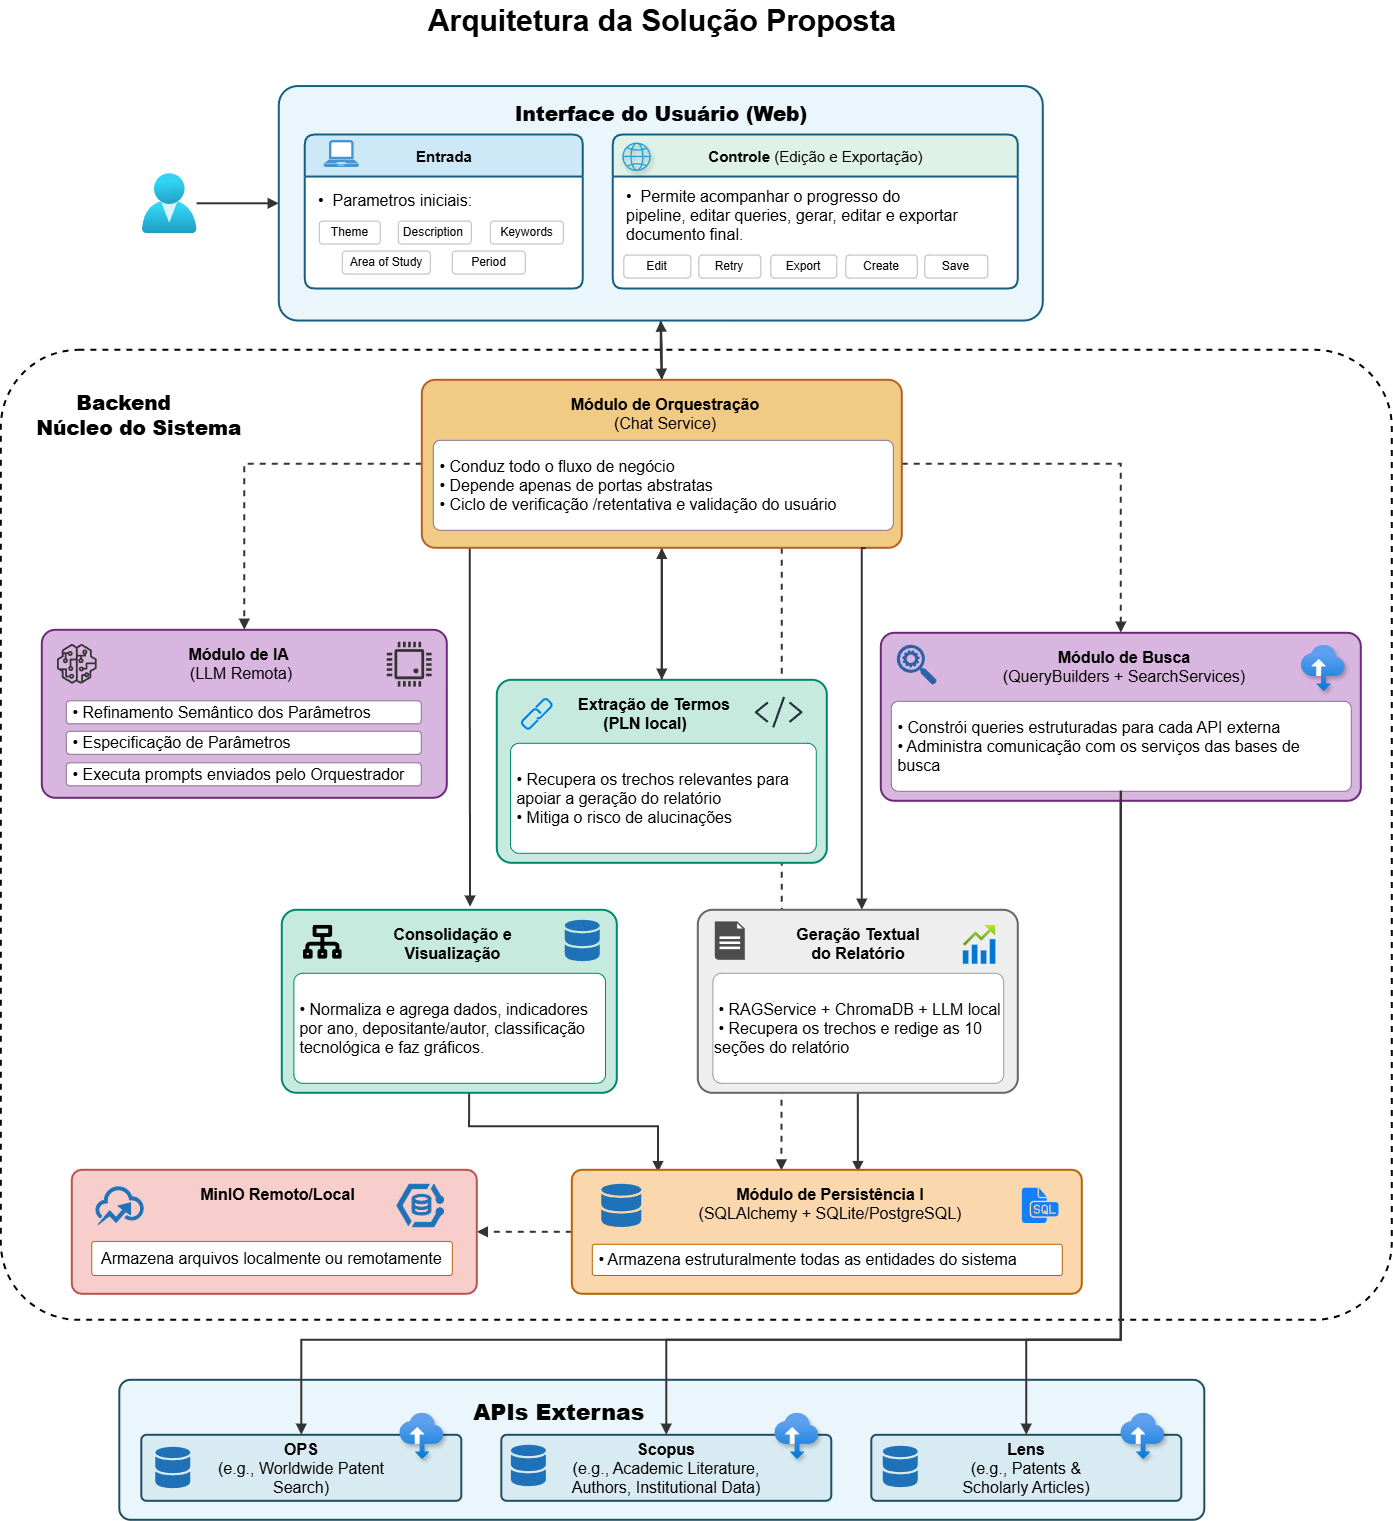
\includegraphics[width=1\textwidth]{img/drawio.png}
    \caption{Arquitetura de módulos do sistema de prospecção tecnológica.}
    \label{fig:arquiterura}
\end{figure}

  \subsection{Especificação de Requisitos}

    \subsubsection{Requisitos Funcionais}
\begingroup
\setlength{\tabcolsep}{10pt}
\begin{longtable}{>{\centering\arraybackslash}p{0.6cm}
                  >{\raggedright\arraybackslash}p{3.2cm}
                  >{\raggedright\arraybackslash}p{8.5cm}}
\toprule
\textbf{Nº} & \textbf{Requisito} & \textbf{Descrição} \\
\midrule
\endfirsthead
\toprule
\textbf{Nº} & \textbf{Requisito} & \textbf{Descrição} \\
\midrule
\endhead
\bottomrule
\endfoot

RF01 & Entrada de parâmetros &
O sistema deve permitir que o usuário informe o tema de pesquisa e parâmetros
complementares (período, área tecnológica, keywords e descrição). \\[4pt] \addlinespace[8pt]

RF02 & Geração de termos de busca &
O sistema deve utilizar um LLM \cite{zhao2023} para gerar automaticamente um
conjunto expandido de termos de busca relacionados ao tema informado, incluindo
sinônimos e variações terminológicas em inglês. \\[4pt] \addlinespace[8pt]

RF03 & Validação iterativa pelo usuário &
O sistema deve apresentar os termos e consultas gerados ao usuário para
validação \cite{white2023}, permitindo aprovação, ajuste ou rejeição antes de
prosseguir para a etapa seguinte. \\[4pt] \addlinespace[8pt]

RF04 & Consulta a bases de patentes &
O sistema deve consultar a API OPS/Espacenet utilizando a linguagem CQL, com
suporte a operadores booleanos, filtros temporais e campos específicos
(título, resumo, classificação CPC/IPC), retornando, por registro, número de
publicação, título, resumo, depositantes, inventores, classificações CPC/IPC,
ano de publicação e status legal; nas buscas de maior volume, o sistema deve
também recuperar as estatísticas já agregadas devolvidas pela API (contagem de
patentes por ano, distribuição por depositante e por classificação CPC), se disponíveis. \\[4pt] \addlinespace[8pt]

RF05 & Consulta a bases de artigos &
O sistema deve consultar a API Scopus, com suporte a operadores
booleanos e filtros por campo (título, resumo, autores, periódico, ano),
retornando, por registro, título, lista de autores e afiliações, resumo, ano de
publicação, periódico ou conferência de origem, número de citações, DOI,
palavras-chave e área de estudo, como lista de itens individuais a serem
agregados pelo próprio sistema, e estatísticas, se disponíveis. \\[4pt] \addlinespace[8pt]

RF06 & Consolidação de metadados &
O sistema deve consolidar os dados retornados pelas diferentes APIs em um
formato interno unificado, realizando deduplicação e normalização dos campos. \\[4pt] \addlinespace[8pt]

RF07 & Geração de indicadores &
O sistema deve calcular indicadores de análise tecnológica: distribuição por
ano, por depositante/autor, por classificação CPC e por área de estudo, conforme dados recuperados. \\[4pt] \addlinespace[8pt]

RF08 & Cálculo e geração de gráficos~S &
O sistema deve ajustar automaticamente uma curva logística à série acumulada
de publicações e patentes recuperadas \cite{fisherpry1971}, calcular os pontos
de leitura do ciclo de vida (GP, MP, SP) e um diagnóstico de confiabilidade do
ajuste, e representar graficamente a curva~S e as demais representações
gráficas padronizadas pela AGITEC. \\[4pt] \addlinespace[8pt]

RF09 & Geração automática de relatório &
O sistema deve gerar automaticamente um relatório técnico consolidado no padrão
REPTEC/AGITEC \cite{agitec2024, reptec2023tetra}, com as oito seções numeradas
do padrão, utilizando RAG \cite{lewis2020} para embasamento factual das seções
redigidas por LLM, com as figuras apresentadas e interpretadas no texto e com
citações restritas aos documentos efetivamente recuperados. \\[4pt] \addlinespace[8pt]

RF10 & Edição e exportação &
O sistema deve disponibilizar o relatório gerado para edição pelo usuário e
permitir sua exportação em LaTeX (incluindo as imagens utilizadas) e em PDF. \\[4pt] \addlinespace[8pt]

RF11 & Rastreamento de métricas &
O sistema deve registrar o consumo de \textit{tokens}, o custo estimado por
operação e o tempo de execução de cada fase do \textit{pipeline}. \\[4pt] \addlinespace[8pt]

RF12 & Revisão do relatório &
O sistema deve revisar o relatório editado, apontando erros de sintaxe LaTeX,
de ortografia, de acentuação e de concordância nos trechos gerados por IA ou
editados pelo usuário, e permitir que cada sugestão seja aplicada ou ignorada
individualmente. \\[4pt] \addlinespace[8pt]

RF13 & Configuração em tempo de execução &
O sistema deve permitir ao usuário escolher o provedor e o modelo de LLM de
cada ponto de uso, as APIs de busca ativas e os parâmetros operacionais, sem
necessidade de reinicialização. \\

\bottomrule
\caption{Requisitos Funcionais do Projeto}
\label{tab:rf}
\end{longtable}

    \subsubsection{Requisitos Não Funcionais}

\begin{longtable}{>{\centering\arraybackslash}p{0.8cm}
                  >{\raggedright\arraybackslash}p{3.2cm}
                  >{\raggedright\arraybackslash}p{8.5cm}}
\toprule
\textbf{Nº} & \textbf{Requisito} & \textbf{Descrição} \\
\midrule
\endfirsthead
\toprule
\textbf{Nº} & \textbf{Requisito} & \textbf{Descrição} \\
\midrule
\endhead
\bottomrule
\endfoot

RNF01 & Modularidade &
A arquitetura deve ser organizada em módulos com responsabilidades bem definidas,
permitindo substituição ou atualização de componentes individuais sem impacto
no restante do sistema. \\[4pt] \addlinespace[8pt]

RNF02 & Extensibilidade &
O sistema deve ser projetado para permitir a integração futura de novas APIs
de busca (Google Patents, arXiv, PubMed) sem necessidade de reescrita
significativa --- requisito diretamente sustentado pela arquitetura hexagonal
descrita na Seção~\ref{sec:hexagonal}. \\[4pt] \addlinespace[8pt]

RNF03 & Desempenho aceitável &
O sistema deve ser capaz de executar o \textit{pipeline} completo em tempo
satisfatório (média de cinco minutos em máquinas comuns), sem dependência de GPU dedicada,
salvo na etapa de geração do relatório, cujo tempo de execução é diretamente
influenciado pelo hardware disponível. \\[4pt] \addlinespace[8pt]

RNF04 & Robustez &
O sistema deve tratar erros de comunicação com APIs externas de forma
transparente ao usuário, realizando novas tentativas ou degradando
graciosamente em caso de falha --- inclusive na ausência de credenciais de LLM
ou de busca configuradas, caso em que o sistema deve permanecer operável por
meio de adaptadores substitutos. \\[4pt] \addlinespace[8pt]

RNF05 & Rastreabilidade &
O sistema deve registrar todas as etapas do processo de prospecção, incluindo
os parâmetros fornecidos, os termos gerados, as consultas construídas e as
validações realizadas pelo usuário. \\[4pt] \addlinespace[8pt]

RNF06 & Controle de custos &
O sistema deve estimar e registrar o custo de cada operação que envolva
chamadas ao LLM \cite{brown2020}, permitindo ao usuário e ao gestor acompanhar
o gasto total associado a cada pesquisa. \\[4pt] \addlinespace[8pt]

RNF07 & Manutenibilidade &
O código deve seguir convenções de estilo e documentação que facilitem sua
manutenção por equipes distintas da que o desenvolveu originalmente. \\

\bottomrule
\caption{Requisitos Não Funcionais do Projeto}
\label{tab:rnf}
\end{longtable}

  \subsection{Especificação da Solução}
  \label{sec:hexagonal}

  A arquitetura do sistema é organizada em camadas e módulos com
responsabilidades bem definidas, seguindo o padrão de \textbf{Arquitetura
Hexagonal} (também chamado \textit{Ports and Adapters}), proposto originalmente
por Cockburn \cite{cockburn2005}. A ideia central do padrão é isolar as regras de
negócio (o "núcleo" da aplicação) de qualquer dependência concreta de
infraestrutura --- bibliotecas de terceiros, clientes HTTP de APIs externas,
SDKs de provedores de LLM --- fazendo com que o núcleo dependa apenas de
contratos abstratos (\textit{ports}), implementados por adaptadores
substituíveis. A Tabela~\ref{tab:camadas} resume as camadas adotadas e exemplos
concretos de cada uma.

\begin{table}[H]
\centering
\caption{Camadas da arquitetura hexagonal adotada}
\label{tab:camadas}
\begin{tabular}{p{2.2cm}p{3.5cm}p{7.5cm}}
\toprule
\textbf{Camada} & \textbf{Responsabilidade} & \textbf{Exemplos} \\
\midrule
Domínio & Tipos de dados puros, sem I/O & Estruturas de resultado de busca, de requisição/resposta de LLM, de termo extraído \\
\textit{Ports} & Contratos (interfaces) dos quais o núcleo depende, sem implementá-los & Porta de LLM; porta de geração de texto; porta de busca de patentes; porta de busca de artigos; porta de repositório; porta de armazenamento de objetos; porta de banco vetorial \\
Serviços (núcleo) & Regras de negócio puras, sem dependência de \textit{framework} & Orquestração do fluxo de prospecção; análise de complexidade de consulta; geração de gráficos; redação, montagem e revisão do relatório; inferência estatística \\
Adaptadores \textit{driven} & Implementam as portas, conectando a integrações reais & Clientes das APIs Anthropic, Gemini e OpenAI-compatível (Ollama/intranet); clientes OPS e Scopus; MinIO; ChromaDB \\
Adaptadores \textit{driving} & Chamam o núcleo a partir do mundo externo & Rotas HTTP (FastAPI) que expõem cada etapa do fluxo ao \textit{frontend} \\
\bottomrule
\end{tabular}
\end{table}

  Na prática, isso significa que o serviço central de orquestração do fluxo
depende de uma porta de LLM e de portas de busca de patentes/artigos --- nunca de
uma biblioteca concreta como o SDK da Anthropic ou o cliente HTTP da OPS. A
implementação concreta de cada porta é decidida e injetada em um único ponto de
composição do sistema, no momento em que a aplicação é inicializada, mantendo o
núcleo de regras de negócio livre de dependências de infraestrutura: mudanças em
uma API externa --- a Lens alterando seu esquema de resposta, a OPS depreciando
um \textit{endpoint}, um novo modelo de LLM sendo lançado --- ficam contidas no
respectivo adaptador, sem exigir alteração do núcleo.

  Vale registrar que essa composição não é feita por meio de um
\textit{framework} de injeção de dependência: trata-se de uma função única de
composição, executada uma vez na inicialização da aplicação, que monta um
dicionário de serviços prontos a partir de duas condições simples --- a
presença de uma credencial configurada e uma \textit{feature flag} que habilita
ou não aquele provedor. Cada fonte de busca (OPS, Scopus, Lens Patents, Lens
Scholarly) só é instanciada e registrada nesse dicionário se estiver habilitada
\emph{e} possuir credencial configurada, o que faz da adição --- ou remoção ---
de uma fonte de busca uma mudança confinada a esse único ponto de composição,
nunca ao serviço de orquestração em si, que já está escrito para operar sobre
uma lista de adaptadores sem saber quantos ou quais existem. Quando nenhuma
credencial de LLM está configurada, esse mesmo ponto de composição realiza um
\textit{fallback} silencioso para um adaptador simulado (\textit{mock}), de
modo que o servidor permaneça operável --- ainda que sem capacidade real de
geração assistida por IA --- em qualquer ambiente, mesmo sem nenhuma
credencial externa disponível; esse comportamento é o que sustenta,
concretamente, o requisito de robustez RNF04.

  Um ponto de atenção,
registrado aqui por rigor metodológico, é que essa inversão de dependência é
mais forte na camada de integrações externas do que na camada de geração de
relatórios: o módulo responsável pelos gráficos é obtido, nas rotas que o
expõem, a partir do mesmo ponto de composição central, mas sem uma porta formal
que o abstraia --- o que é aceitável, já que hoje existe apenas uma implementação
de geração de relatório, mas que representa uma aplicação apenas parcial do
princípio de inversão de dependência nessa camada específica, distinta da
aplicação mais completa observada nas integrações de LLM e de busca.

  Essa organização em camadas está diretamente fundamentada nos princípios
\textbf{SOLID} de projeto orientado a objetos, formalizados por Martin
\cite{martin2002} e posteriormente sistematizados em torno do princípio de
inversão de dependência como eixo central de arquiteturas em camadas
\cite{martin2017}. Dos cinco princípios, o \textbf{Princípio da Responsabilidade
Única} (\textit{Single Responsibility Principle}, SRP) se manifesta na
granularidade dos serviços do núcleo: o componente que orquestra o fluxo de
prospecção não calcula complexidade de consulta, o componente que calcula
complexidade de consulta não gera gráficos, e o componente que gera gráficos não
sabe nada sobre LLMs --- cada um tem um único motivo para mudar. O
\textbf{Princípio Aberto-Fechado} (\textit{Open-Closed Principle}, OCP) aparece
no mecanismo de registro de construtores de consulta por API: uma nova fonte de
busca é adicionada registrando um novo construtor em um ponto único de
extensão, sem modificar o código dos construtores já existentes. O
\textbf{Princípio da Substituição de Liskov} (\textit{Liskov Substitution
Principle}, LSP) garante que qualquer construtor de consulta, seja para o OPS,
o Scopus ou o Lens, respeite o mesmo contrato de entrada e saída e possa ser
utilizado pelo serviço de orquestração de forma intercambiável, sem que este
precise saber qual API está por trás de cada um. O \textbf{Princípio da
Segregação de Interface} (\textit{Interface Segregation Principle}, ISP) se
reflete na existência de portas estreitas e específicas --- uma porta apenas
para chamadas de LLM, portas distintas para busca de patentes e de artigos ---
em vez de uma única interface genérica que obrigasse cada adaptador a
implementar métodos que não utiliza.

  O princípio mais visivelmente ligado à escolha arquitetural do projeto,
contudo, é o \textbf{Princípio da Inversão de Dependência} (\textit{Dependency
Inversion Principle}, DIP), segundo o qual módulos de alto nível não devem
depender de módulos de baixo nível --- ambos devem depender de abstrações
\cite{martin2017}. O serviço central de orquestração depende de uma porta de
LLM e de portas de busca de patentes/artigos --- abstrações definidas pelo
próprio domínio do sistema --- e nunca de bibliotecas concretas como o SDK da
Anthropic ou o cliente HTTP da OPS; a implementação concreta é decidida e
injetada no ponto de composição da aplicação, mantendo o núcleo de negócio
livre de dependências de infraestrutura, exatamente na direção descrita na
justificativa original da arquitetura hexagonal do projeto: mudanças em APIs
externas "ficam contidas nos adaptadores --- o núcleo não sabe que aconteceu
nada". O módulo de geração de relatório, como já observado, segue uma versão
mais modesta do mesmo princípio: é obtido a partir do ponto de composição
central em vez de instanciado diretamente pelas rotas que o utilizam, invertendo
o controle de construção, mas sem uma porta/contrato formal que o abstraia --- a
diferença é que, ao contrário do serviço de orquestração, não há hoje
necessidade real de múltiplos "provedores de relatório", o que torna essa
aplicação parcial do DIP uma escolha aceitável, e não uma inconsistência de
projeto. A Tabela~\ref{tab:solid} sintetiza onde cada princípio é observado.

\begin{table}[H]
\centering
\caption{Princípios SOLID observados na arquitetura do sistema}
\label{tab:solid}
\begin{tabular}{p{1.6cm}p{5.2cm}p{6.4cm}}
\toprule
\textbf{Princípio} & \textbf{Onde é observado} & \textbf{Exemplo} \\
\midrule
SRP & Granularidade dos serviços do núcleo & Orquestração, análise de complexidade e geração de gráficos são serviços distintos \\
OCP & Registro extensível de construtores de consulta & Nova API de busca = novo construtor registrado, sem alterar os existentes \\
LSP & Contrato único entre construtores de consulta & Qualquer construtor (OPS, Scopus, Lens) é substituível pelo serviço de orquestração \\
ISP & Portas estreitas e específicas & Porta de LLM separada de portas de busca de patentes/artigos \\
DIP & Núcleo dependendo de abstrações, não de implementações & Serviço de orquestração $\rightarrow$ porta de LLM/busca (forte); rota de relatório $\rightarrow$ classe concreta (parcial) \\
\bottomrule
\end{tabular}
\end{table}

\begin{figure}[H]
    \centering
    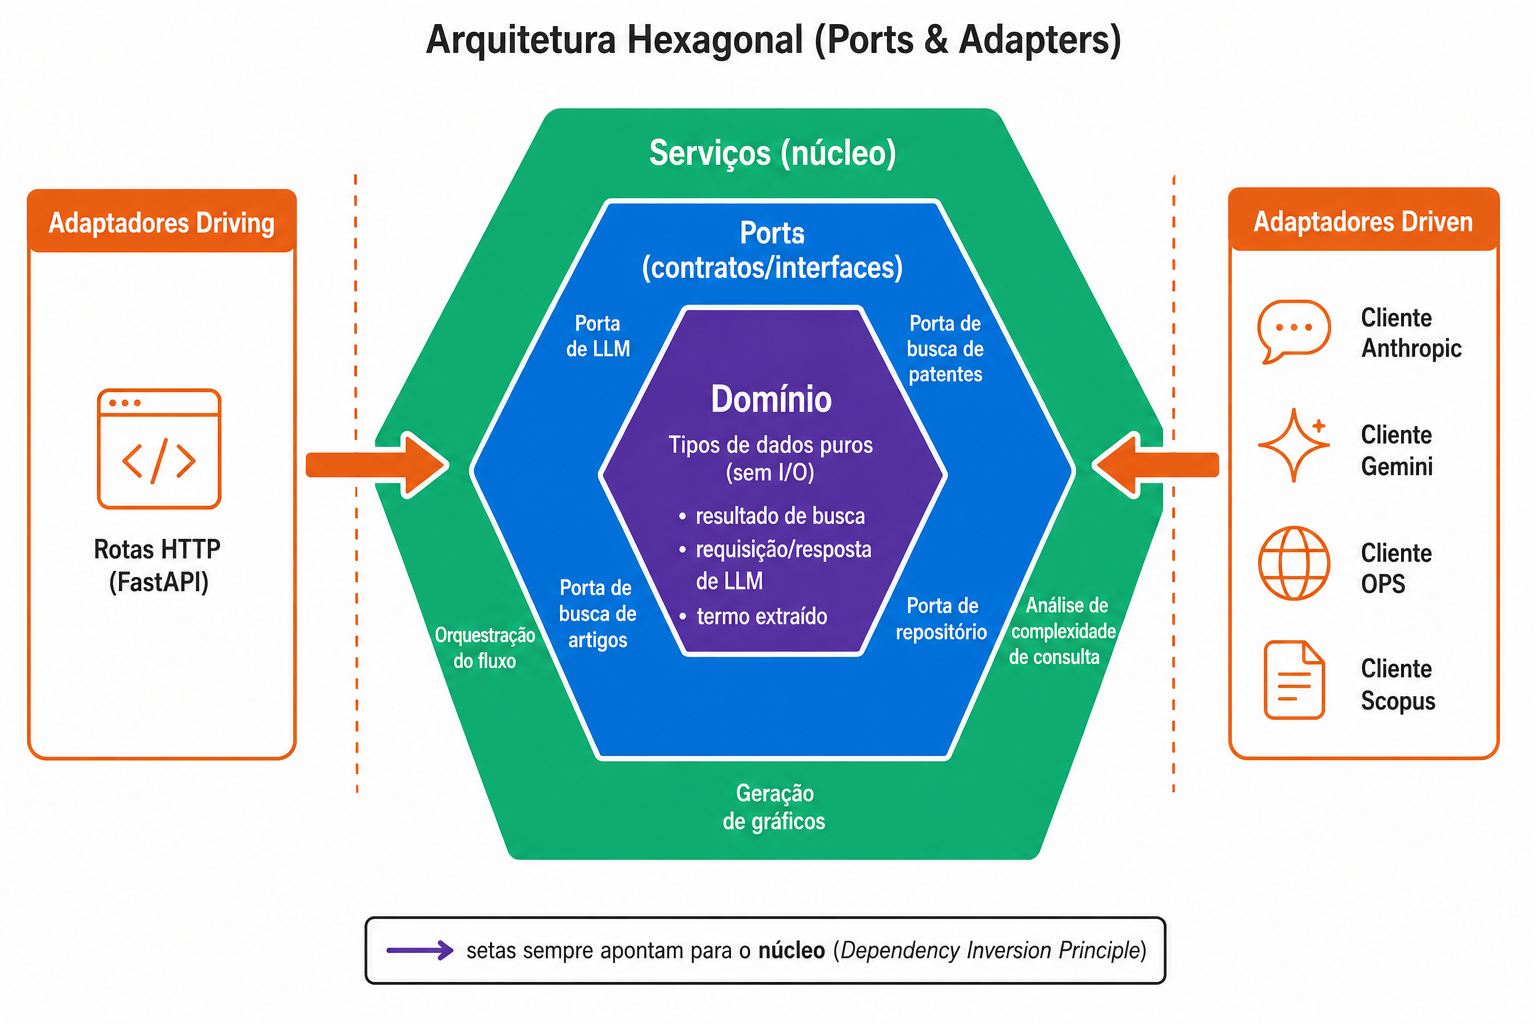
\includegraphics[width=0.85\textwidth]{img/arquitetura_hexagonal_camadas.png}
    \caption{Camadas da arquitetura hexagonal: domínio, \textit{ports}, serviços e adaptadores \textit{driven}/\textit{driving}.}
    \label{fig:hexagonal-camadas}
\end{figure}

  A Figura~\ref{fig:fluxograma} apresenta o fluxo geral de operação do sistema.
O usuário inicia o processo enviando os parâmetros
iniciais da pesquisa por meio da interface \textit{web}. Caso deseje refiná-los, a
aplicação aciona o módulo de IA, que gera novas variações do tema
\cite{white2023}; esse ciclo se repete até que o usuário esteja satisfeito com
o tema gerado, cujo histórico é armazenado para rastreabilidade.

\begin{figure}[H]
    \centering
    \includegraphics[width=1\textwidth]{img/fluxograma.png}
    \caption{Fluxo geral do sistema de prospecção tecnológica.}
    \label{fig:fluxograma}
\end{figure}

Com os parâmetros aprovados, o sistema realiza o \textit{fetch} nas APIs
externas e executa uma busca inicial, indexando os documentos recuperados. A
partir desses documentos, o pipeline local de PLN sugere um conjunto de termos
relevantes ao usuário (Seção~\ref{sec:extracao-termos}), que pode aprová-los ou
editá-los --- ciclo que também é registrado em histórico. Com os termos
definidos, o módulo de IA constrói uma nova \textit{query}, que é apresentada
ao usuário para validação antes da execução da busca final.

Concluída a busca final, a aplicação gera automaticamente os gráficos de análise
\cite{foster1986, fisherpry1971} --- restritos ao conjunto de figuras previsto no
padrão REPTEC --- e seus resumos numéricos. Os gráficos, juntamente com os dados
consolidados e o histórico do processo, alimentam a etapa de síntese de dados,
que embasa a geração automática do relatório no padrão REPTEC \cite{lewis2020,
agitec2024, reptec2023tetra}, seção a seção. O relatório é então disponibilizado
como arquivo LaTeX editável na própria interface, onde o usuário pode inserir
novas imagens, revisar o texto, compilar o PDF e exportar o resultado, cabendo a
ele a edição e a validação final antes da entrega.

  \subsection{Configurações e Parâmetros Adotados}

  No sistema desenvolvido, a fase de maturidade da curva~S é determinada
automaticamente ajustando uma função logística à série acumulada de patentes e
artigos recuperados (Seção~\ref{sec:curva-s}), e não por um limiar arbitrário
sobre a taxa de crescimento ano a ano. A partir dos parâmetros $K$, $r$ e $t_0$
desse ajuste, o sistema calcula os pontos de leitura GP, MP e SP por inversão
algébrica da função logística, acompanhados de um diagnóstico de confiabilidade
baseado em $R^2$ e em critérios de plausibilidade da taxa de crescimento
estimada. Esse método já possui precedente de aplicação real na prática da
AGITEC, como demonstrado com dados reais de patentes e publicações sobre a
tecnologia TETRA em \cite{reptec2023tetra}. A representação gráfica
da curva~S, gerada automaticamente a partir dos dados de publicação por ano, é
incluída no relatório final como elemento de análise estratégica, junto do aviso
de confiabilidade do ajuste quando aplicável. O estágio do ciclo de vida
(emergente, crescimento, maturidade ou saturação) é determinado por código a
partir da posição do último ano observado em relação a GP, MP e SP; o estágio
geral da tecnologia segue a curva de patentes, e é informado ao LLM como um
fato pronto, em vez de ser inferido por ele.

  Os modelos de linguagem são configurados por \textbf{ponto de uso}, em
tabelas próprias do banco de dados: cada um dos cinco pontos de uso
(variações de tema, consulta exploratória, consulta final, redação do
relatório e revisão do relatório) aponta para uma configuração de provedor,
modelo e credencial. Os testes locais foram realizados com os modelos
\textbf{Qwen~2.5~(3B-instruct)} e \textbf{Gemma~3~(4B)}, disponibilizados por
meio da plataforma \textbf{Ollama}, com geração de até 4.096 \textit{tokens} por
chamada. Parâmetros operacionais --- como o número de fragmentos recuperados
por seção, o corte relativo de relevância do RAG e o idioma da revisão
ortográfica --- ficam em uma tabela de configurações editável pela interface,
com valores iniciais semeados de forma idempotente, sem sobrescrever valores já
alterados pelo usuário.

  A engenharia de \textit{prompt} (Seção~\ref{sec:hexagonal} e Capítulo~2) é
empregada em
múltiplas etapas do \textit{pipeline}: na geração de variações do tema, na
construção de consultas para as APIs externas e na geração de cada seção do
relatório técnico. Os \textit{prompts} são estruturados para instruir
explicitamente o modelo a basear suas respostas exclusivamente nos dados
recuperados, evitando a introdução de informações não verificadas.

  O RAG local (Seção~\ref{sec:rag} do Capítulo~2) opera da seguinte forma: o
título e o resumo de cada documento da busca final (patentes e artigos
científicos) são divididos em fragmentos (\textit{chunks}) de 1000
caracteres com sobreposição de 200 caracteres e convertidos em
\textit{embeddings} pelo mesmo modelo Sentence-BERT \cite{reimers2019} usado
nos filtros de relevância. Esses vetores são armazenados em uma coleção do
ChromaDB, com o identificador da sessão, a citação e a referência ABNT do
documento de origem nos metadados. Na etapa de geração de cada seção do
relatório, o sistema formula uma \textit{query} semântica a partir do tema e do
propósito da seção, recupera os cinco fragmentos mais similares da sessão por
similaridade de cosseno, descarta os que ficarem abaixo de $75\%$ do escore do
mais relevante e injeta o restante, como texto puro, no \textit{prompt} enviado
ao LLM local, junto da lista de citações permitidas --- caracterizando a
variante de RAG Naive local descrita na Seção~\ref{sec:rag}.

  \subsection{Tecnologias Adotadas}

  Para a implementação do sistema, as seguintes tecnologias foram selecionadas:

  O \textit{backend} foi desenvolvido em \textbf{Python}, com o
\textit{framework} \textbf{FastAPI}, escolhido por sua alta performance em
operações assíncronas e pela geração automática de documentação interativa
(Swagger/OpenAPI). A persistência relacional é gerenciada pelo ORM
\textbf{SQLAlchemy}, com \textbf{PostgreSQL} como banco de dados (o SQLite é
empregado apenas nos testes automatizados). A busca vetorial e a persistência
de \textit{embeddings} são realizadas pelo \textbf{ChromaDB} \cite{gao2024}, e
os artefatos binários, pelo \textbf{MinIO}. A execução local dos modelos
de linguagem é viabilizada pelo \textbf{Ollama} \cite{zhao2023}, e os
\textit{embeddings} são gerados com a biblioteca \textbf{sentence-transformers}
\cite{reimers2019}. O pipeline local de extração de termos (Seção~4.3) emprega
\textbf{spaCy} e \textbf{KeyphraseVectorizers} (PatternRank) \cite{schopf2022},
\textbf{BM25F} \cite{robertson2004}, \textbf{KeyBERT} \cite{grootendorst2020},
RRF \cite{cormack2009} e C-value \cite{frantzi2000}. As consultas às APIs externas
são realizadas por meio de requisições HTTP com a biblioteca \textbf{httpx}, com
suporte a requisições assíncronas, controle de taxa e novas tentativas em caso
de falha de rede. Os gráficos são gerados com \textbf{matplotlib} e o ajuste da
curva~S, com \textbf{SciPy}. O relatório é renderizado a partir de um
\textit{template} \textbf{Jinja2} e compilado por um serviço \textbf{TeX Live}
dedicado; a revisão ortográfica e gramatical utiliza o \textbf{LanguageTool}.
Todos os serviços de infraestrutura --- PostgreSQL, MinIO, ChromaDB, Ollama,
TeX Live e LanguageTool --- são orquestrados localmente por \textbf{Docker
Compose}.

  A interface \textit{web} do sistema é desenvolvida com \textbf{React}, utilizando o \textbf{Vite} como ferramenta de \textit{build} e ambiente de desenvolvimento, o \textbf{Zustand} para gerenciamento de estado e o \textbf{Tailwind CSS} para a construção da camada visual. Essa escolha busca proporcionar uma aplicação responsiva, modular e de fácil manutenção. Entre as funcionalidades disponíveis na interface, destacam-se o assistente guiado (\textit{wizard}) de quatro etapas para condução de toda a pesquisa, a edição manual dos campos de consulta em cada etapa, o registro de auditoria do uso de IA por sessão, a tela de configurações e, na última etapa, o formulário do relatório e o editor LaTeX com painel de imagens, revisão, compilação em PDF e exportação, conforme detalhado na Seção~\ref{sec:estado-atual}.

  A persistência de artefatos gerados (gráficos, figuras fixas, anexos, \texttt{.tex} e PDF) utiliza o \textbf{MinIO}, executado em um contêiner Docker local, no mesmo padrão empregado para o PostgreSQL, e configurável para apontar ou replicar para a instância remota do MinIO do Exército --- permitindo que o desenvolvimento local funcione de forma independente, mas com um caminho claro de promoção para o ambiente institucional real.

%% TODO (imagem pendente): diagrama simples do plano de persistência MinIO
%% (contêiner local <-> instância remota do Exército).
% \begin{figure}[H]
%     \centering
%     
\includegraphics[width=0.8\textwidth]{img/plano_persistencia_minio.png}
%     \caption{Plano de persistência de artefatos via MinIO: contêiner local e caminho de promoção para a instância remota do Exército.}
%     \label{fig:plano-minio}
% \end{figure}

  \subsection{Modelagem do Banco de Dados}
  \label{sec:modelagem-bd}

  O modelo de dados relacional do sistema é implementado com o ORM
\textbf{SQLAlchemy} em sua API assíncrona declarativa, versionado por
migrações \textbf{Alembic}, com \textbf{PostgreSQL} como banco de dados
(Seção~\ref{sec:hexagonal}). O
esquema ativo é organizado em torno de uma entidade central ---
\texttt{research\_session} ---, que representa uma execução completa do fluxo
de prospecção (Figura~\ref{fig:fluxograma}) e da qual derivam, por chave
estrangeira, as demais entidades do domínio: os parâmetros de entrada da
sessão, as \textit{queries} de busca geradas, o registro de chamadas de IA,
as seções e o manifesto do relatório e, indiretamente, por meio das
\textit{queries}, os documentos de patente e artigo recuperados e os gráficos
gerados. Um segundo grupo, independente das sessões, armazena as
configurações editáveis em tempo de execução. A Tabela~\ref{tab:entidades-bd}
resume as entidades do esquema ativo e seu papel no domínio.

\begin{table}[H]
\centering
\caption{Entidades do esquema relacional ativo}
\label{tab:entidades-bd}
\begin{tabular}{p{3.2cm}p{9.9cm}}
\toprule
\textbf{Entidade} & \textbf{Papel} \\
\midrule
\texttt{research\_session} & Entidade central (\textit{hub}); uma linha por execução do fluxo de prospecção, com a etapa corrente do assistente para retomada no ponto certo \\
\texttt{session\_input} & Parâmetros de entrada da sessão; auto-relacionada (tema original vs.\ variante refinada por IA) \\
\texttt{session\_probe\_query} & \textit{Queries} de busca por fonte (OPS, Scopus); auto-relacionada (\textit{query} de exploração inicial vs.\ \textit{query} final escolhida) \\
\texttt{session\_ai\_call} & Registro (\textit{log}) somente-inserção de cada chamada de IA feita durante o assistente guiado \\
\texttt{patent}\slash\texttt{article} & Documentos recuperados, deduplicados globalmente por \texttt{dedup\_key}, independentemente de sessão ou \textit{query} \\
\texttt{probe\_query\_patent}\newline\texttt{probe\_query\_article} & Entidades associativas que resolvem o relacionamento muitos-para-muitos entre \textit{queries} e documentos \\
\texttt{probe\_query\_term} & Termos extraídos por PLN local a partir dos documentos de uma \textit{query} de exploração \\
\texttt{session\_chart} & Gráfico gerado para uma \textit{query} final: chave do PNG no MinIO e resumo numérico (JSON) usado na redação do relatório \\
\texttt{session\_report\_}\allowbreak\texttt{section} & Uma seção do relatório: contexto recuperado pelo RAG, texto gerado e fontes citáveis (JSON) \\
\texttt{session\_report} & Manifesto do relatório da sessão: chaves do \texttt{.tex} e do PDF no MinIO e dados do formulário \\
\texttt{app\_settings},\newline \texttt{llm\_provider\_}\allowbreak\texttt{configs},\newline \texttt{llm\_call\_site\_}\allowbreak\texttt{bindings},\newline \texttt{search\_api\_}\allowbreak\texttt{selection} & Configurações editáveis em tempo de execução: parâmetros operacionais, provedores/modelos de LLM, vínculo de cada ponto de uso e APIs de busca ativas \\
\bottomrule
\end{tabular}
\end{table}

  \textbf{Auto-relacionamentos.} Duas entidades do esquema empregam um
relacionamento reflexivo (unário), no qual uma linha referencia outra linha da
mesma tabela por meio de uma chave estrangeira opcional que aponta para a
própria chave primária --- um padrão clássico de modelagem para representar
hierarquias ou histórico de revisão dentro de uma única tabela
\cite{chen1976}. Em \texttt{session\_input}, a linha raiz (\texttt{parent\_id}
nulo) é o tema bruto submetido pelo usuário; se o usuário aciona o refino
assistido por IA (Seção~\ref{sec:hexagonal}), a variante escolhida para
prosseguir é persistida como uma segunda linha, com \texttt{parent\_id}
apontando para a linha raiz. Em \texttt{session\_probe\_query}, o mesmo padrão
distingue a \textit{query} de exploração inicial (\texttt{tipo} nulo) da
\textit{query} final escolhida pelo usuário, gravada como uma nova linha com
\texttt{parent\_id} apontando para a linha de exploração da mesma fonte e
\texttt{tipo} preenchido com a variante selecionada (específica, balanceada ou
ampla). Esse desenho evita duplicar o esquema da tabela de \textit{queries}
para cada etapa do fluxo --- uma aplicação, na camada de persistência, do
mesmo espírito de extensão sem duplicação discutido a propósito do Princípio
Aberto-Fechado (Seção~\ref{sec:hexagonal}) ---, com a restrição de unicidade
da tabela ajustada para considerar sessão, fonte de busca e tipo em conjunto
(\texttt{UNIQUE(session\_id, fonte, tipo)}), de modo que cada combinação
exista no máximo uma vez. Não há, portanto, um banco ou um conjunto de tabelas
literalmente separado para "exploratório" e "final": as duas etapas
compartilham a mesma tabela, distinguidas apenas por qual linha cada uma é e
para qual linha ela aponta.

  \textbf{Relacionamentos muitos-para-muitos.} Uma mesma patente ou artigo
pode ser recuperado por mais de uma \textit{query} --- por exemplo, quando a
\textit{query} de exploração inicial e a \textit{query} final da mesma fonte
retornam parcialmente o mesmo conjunto de documentos --- e uma mesma
\textit{query} recupera, tipicamente, dezenas de documentos distintos,
caracterizando um relacionamento muitos-para-muitos entre
\texttt{session\_probe\_query} e \texttt{patent}/\texttt{article}. Como o par
(\textit{query}, documento) carrega um atributo próprio --- o
\texttt{relevance\_score} daquele documento especificamente em relação àquela
\textit{query}, que não pertence nem à \textit{query} isoladamente nem ao
documento isoladamente ---, o relacionamento não é resolvido por uma simples
chave estrangeira, mas por uma \textbf{entidade associativa} (tabela de
junção) dedicada --- \texttt{probe\_query\_patent} e
\texttt{probe\_query\_article} ---, cada uma com restrição de unicidade sobre
o par de chaves estrangeiras, o padrão canônico para modelar relacionamentos
N:N com atributos próprios do relacionamento \cite{chen1976, codd1970}. A
deduplicação em si acontece em um nível anterior ao relacionamento:
\texttt{patent} e \texttt{article} têm \texttt{dedup\_key} como coluna única,
de modo que o mesmo documento --- identificado pela combinação de fonte e
identificador de registro na fonte --- gera sempre uma única linha na tabela
de documentos, não importa quantas \textit{queries} ou sessões diferentes o
recuperem; o que se multiplica, nesse caso, são as linhas da tabela
associativa, cada uma amarrando aquele documento a uma \textit{query}
específica que o encontrou. Por contraste, os termos extraídos por PLN
(\texttt{probe\_query\_term}) não são deduplicados nem compartilhados entre
\textit{queries}: cada termo só tem sentido no contexto da \textit{query} que
o gerou, o que dispensa uma entidade associativa e justifica um
relacionamento um-para-muitos simples entre \texttt{session\_probe\_query} e
\texttt{probe\_query\_term}.

  A Tabela~\ref{tab:relacionamentos-bd} sintetiza os tipos de relacionamento
empregados no esquema e onde cada um ocorre.

\begin{table}[H]
\centering
\caption{Tipos de relacionamento no esquema relacional ativo}
\label{tab:relacionamentos-bd}
\begin{tabular}{p{3.0cm}p{5.3cm}p{4.6cm}}
\toprule
\textbf{Tipo} & \textbf{Onde ocorre} & \textbf{Observação} \\
\midrule
Um-para-muitos & \texttt{research\_session} $\rightarrow$\newline \texttt{session\_input},\newline \texttt{session\_probe\_query},\newline \texttt{session\_ai\_call},\newline \texttt{session\_report\_section};\newline \texttt{session\_probe\_query} $\rightarrow$\newline \texttt{session\_chart} & Exclusão em cascata (\textit{cascade delete-orphan}) a partir da sessão \\
Um-para-um & \texttt{research\_session} $\rightarrow$\newline \texttt{session\_report} & Um único relatório montado por sessão, sobrescrito a cada nova montagem \\
Auto-relacionamento (unário, opcional) & \texttt{session\_input}.\texttt{parent\_id};\newline \texttt{session\_probe\_query}.\texttt{parent\_id} & Distingue estágios do fluxo (raiz/exploração vs.\ variante/final) dentro da mesma tabela \\
Muitos-para-muitos com atributo (entidade associativa) & \texttt{session\_probe\_query} $\leftrightarrow$ \texttt{patent}\slash\texttt{article}, via\newline \texttt{probe\_query\_patent}\newline \texttt{probe\_query\_article} & \texttt{relevance\_score} é atributo do par \textit{query}--documento, não de nenhum dos dois isoladamente \\
Deduplicação global (unicidade) & \texttt{patent}.\texttt{dedup\_key};\newline \texttt{article}.\texttt{dedup\_key} & Garante uma única linha por documento, ainda que recuperado por múltiplas \textit{queries} ou sessões \\
\bottomrule
\end{tabular}
\end{table}

%% TODO (imagem pendente): diagrama entidade-relacionamento do esquema ativo
%% (research_session como hub, auto-relacionamentos em session_input e
%% session_probe_query, tabelas associativas patent/article).
\begin{figure}[H]
    \centering
    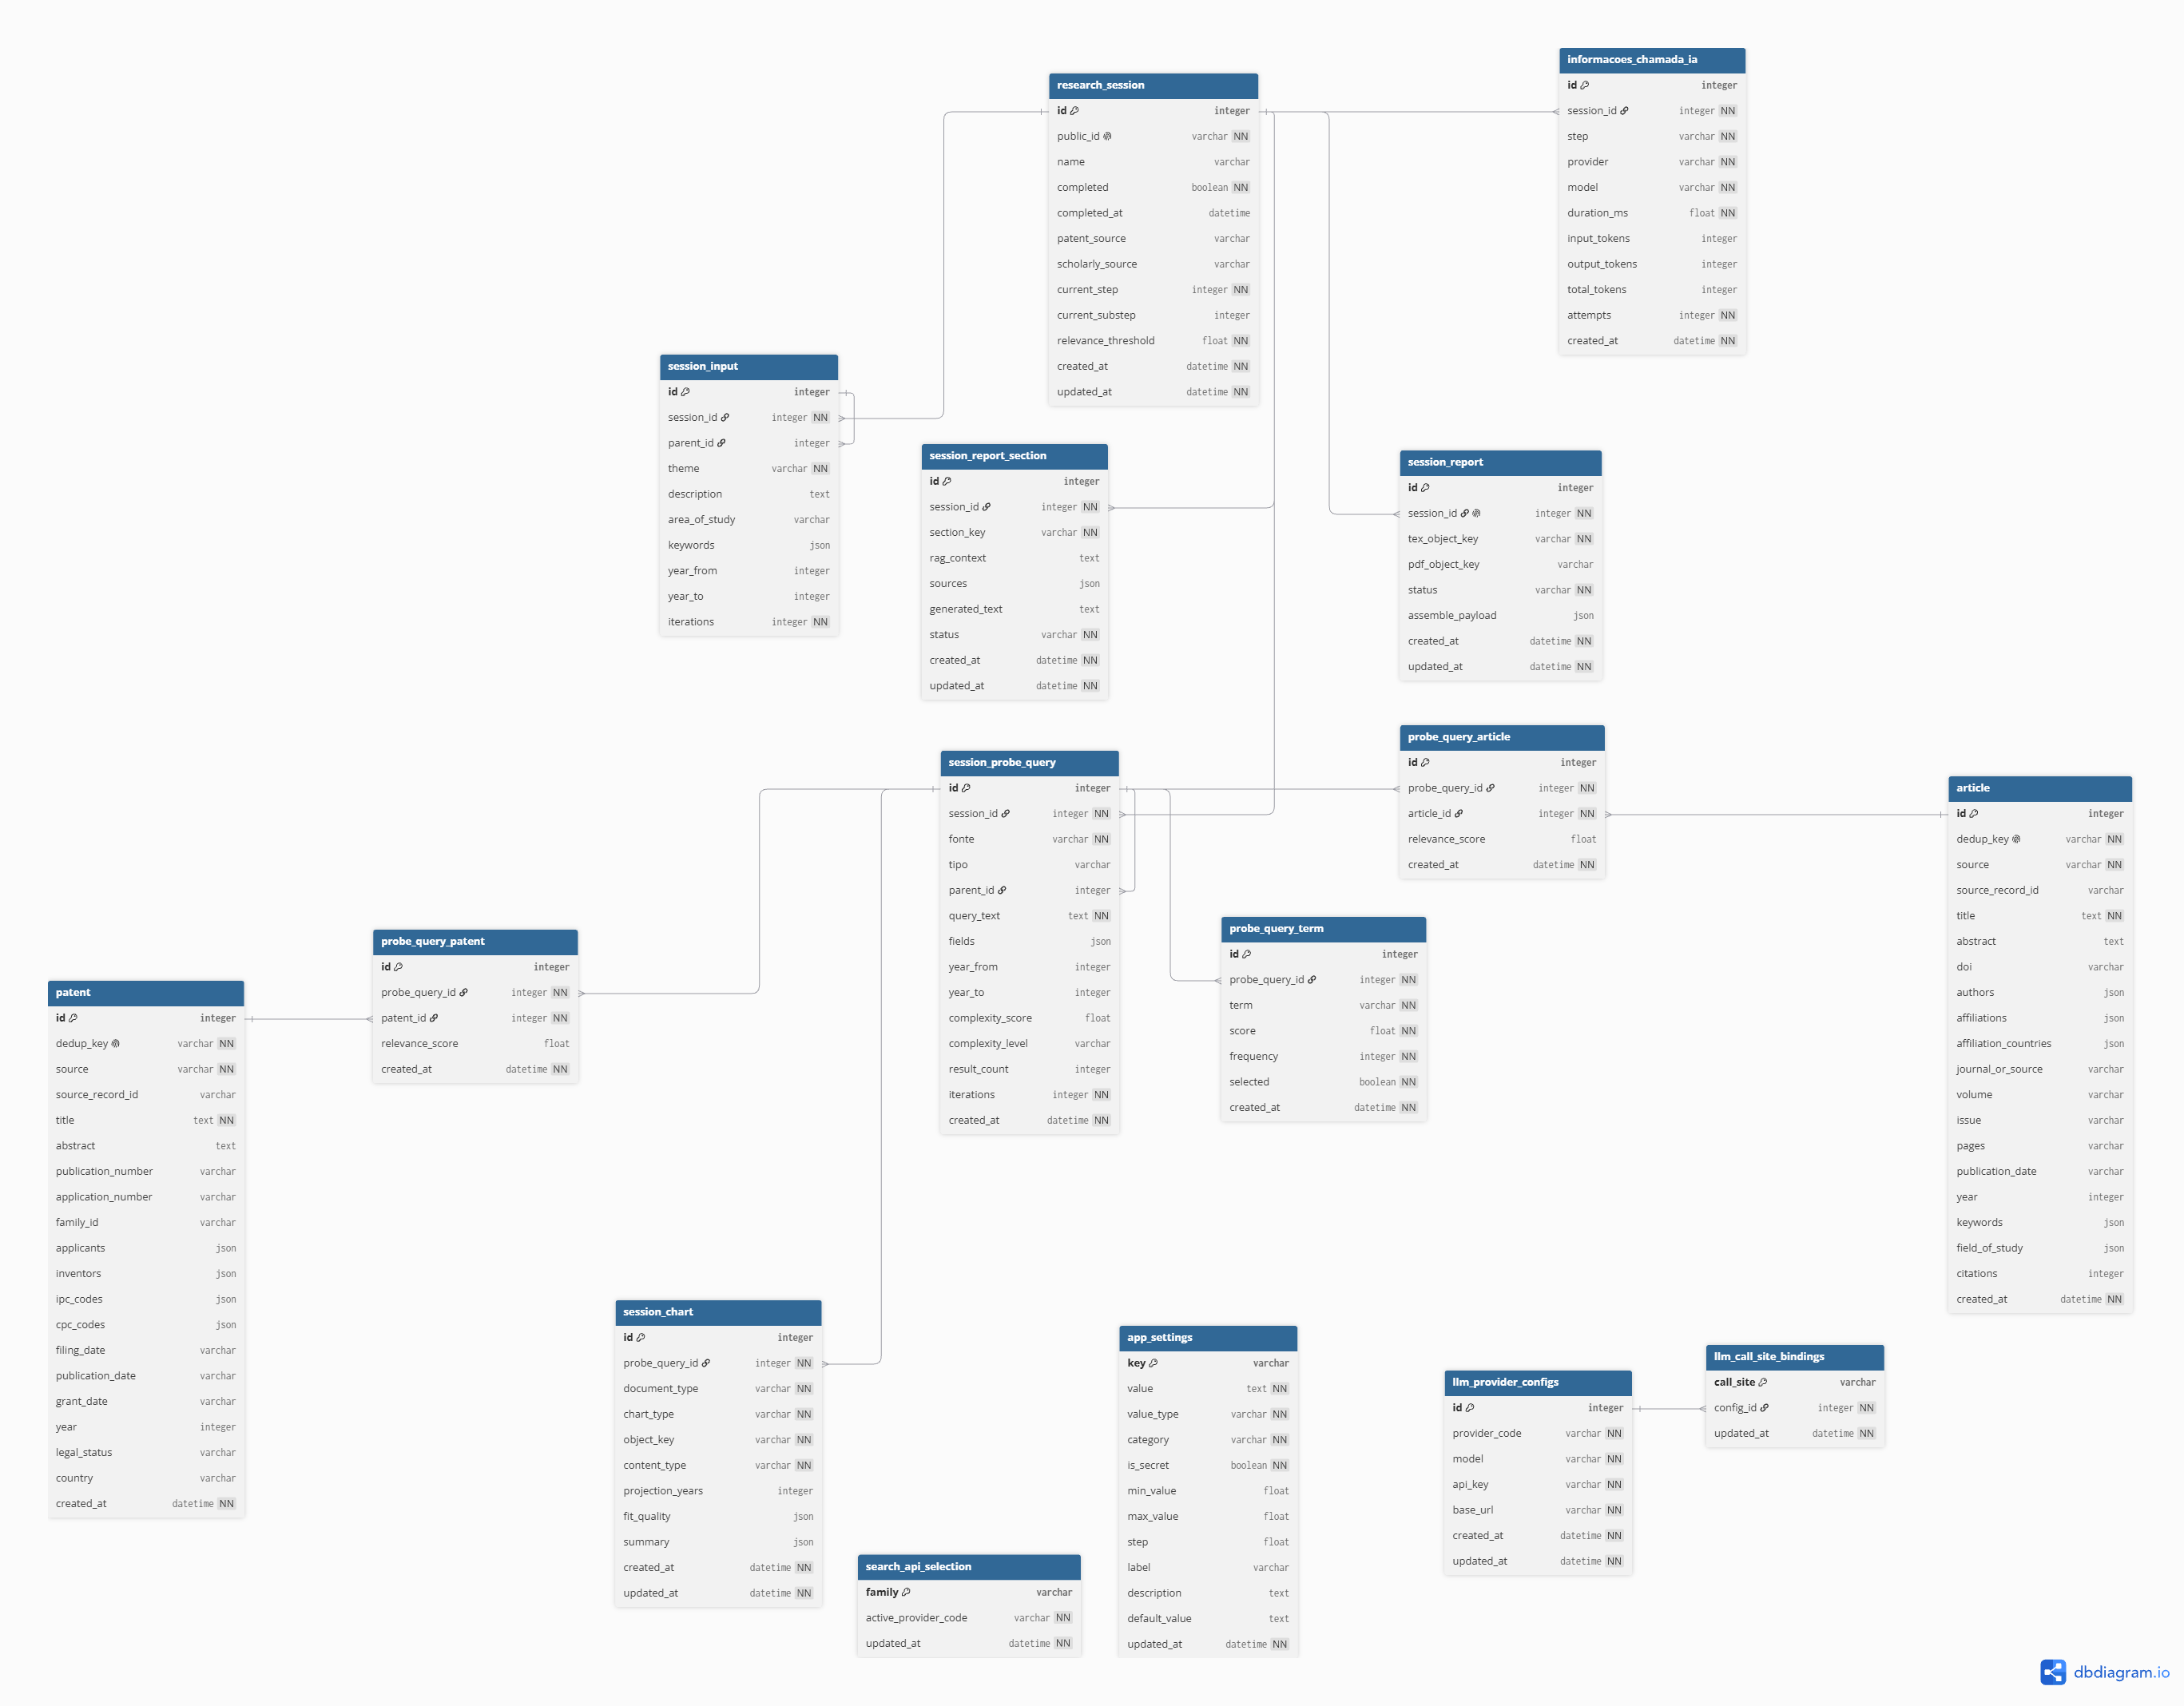
\includegraphics[width=1\textwidth]{img/modelo_dados_der.png}
    \caption{Diagrama entidade-relacionamento do núcleo do esquema relacional ativo (sessões, consultas e documentos). As tabelas de gráficos, relatório e configurações estão descritas na Tabela~\ref{tab:entidades-bd}.}
    \label{fig:modelo-dados-der}
\end{figure}

  \subsection{Estado Atual de Desenvolvimento}
  \label{sec:estado-atual}

  No estágio atual do projeto, o protótipo desenvolvido contempla, de ponta a
ponta, as seguintes funcionalidades implementadas e testadas:

  \textbf{Arquitetura e estrutura do \textit{backend}:} a API REST com FastAPI está estruturada
segundo o padrão de arquitetura hexagonal descrito na
Seção~\ref{sec:hexagonal}, com os \textit{endpoints} de interação com IA e
busca (\texttt{/api/v1/chat/*}), de gerenciamento de sessões
(\texttt{/api/v1/research-session/*} e \texttt{/api/v1/session-input/*}), de
geração de gráficos e do relatório (\texttt{/api/v1/report/*}), de inferência
estatística (\texttt{/api/v1/inference/*}) e de configuração
(\texttt{/api/v1/config/*}) implementados e documentados via Swagger. O modelo
de dados ativo segue o esquema relacional detalhado na
Seção~\ref{sec:modelagem-bd}, implementado com SQLAlchemy assíncrono e
gerenciado por migrações versionadas (Alembic), com PostgreSQL como banco de
dados. Os módulos puros do núcleo (complexidade de consulta, curva~S,
estatística, posicionamento de figuras, citações, validação e revisão de texto)
são cobertos por testes unitários automatizados.

  \textbf{Integração com OPS, Scopus e Lens:} os construtores de consulta e
serviços de busca para OPS e Scopus foram implementados e testados com consultas reais,
validando a capacidade de recuperação de patentes e artigos a partir de termos
fornecidos, incluindo o mecanismo de verificação automática da complexidade
estrutural de cada consulta antes do envio, com nova tentativa e simplificação
assistida por LLM em caso de consulta excessivamente complexa. O tratamento de
erros, paginação, controle de taxa e novas tentativas em falhas de rede estão
implementados para ambas as APIs, e a busca final distingue o total real de
documentos informado pela base da amostra efetivamente analisada. Os
construtores de consulta da plataforma Lens estão implementados, mas a fonte
ainda não é exposta na interface do usuário.

  \textbf{Extração de termos:} implementada como um pipeline local de
Processamento de Linguagem Natural (PatternRank, BM25F, KeyBERT, RRF e
C-value), sem uso de LLM nesta etapa específica
(Seção~\ref{sec:extracao-termos}), conectado à interface de seleção de termos
apresentada ao usuário. O pipeline substituiu uma primeira versão baseada em
\textit{noun chunks}, TF-IDF e KeyBERT combinados linearmente.

  \textbf{Geração de gráficos e curva~S:} implementada e conectada a rotas
dedicadas, que geram as figuras previstas no padrão REPTEC --- volume anual,
principais depositantes e instituições, quadros das classificações CPC e das
áreas de estudo mais frequentes e curvas~S de patentes e de artigos com os
pontos GP/MP/SP e o diagnóstico de confiabilidade do ajuste
(Seção~\ref{sec:curva-s}) ---, a partir dos documentos já persistidos da busca
final da sessão. Nomes de depositantes ou instituições com mais de 45
caracteres são abreviados automaticamente, para não distorcer os gráficos.

  \textbf{Estimação de completude amostral e estabilidade de \textit{ranking}
(Chao1/\textit{bootstrap}):} implementada como uma rota de inferência
estatística sobre a busca final (Seção~\ref{sec:chao1bootstrap}), que
enriquece iterativamente a amostra até sua saturação ou até o limite de tempo
configurado.

  \textbf{RAG local e geração do relatório:} implementados e conectados a
rotas de produção. A indexação dos documentos da busca final no ChromaDB, a
recuperação por similaridade com corte relativo de relevância e a redação das
seções por LLM local são executadas seção a seção; as seções de texto fixo,
as figuras, as citações, o quadro de busca, as assinaturas e a bibliografia
são produzidos de forma determinística, e o \texttt{.tex} resultante segue o
\textit{template} REPTEC (Seção~\ref{sec:fase5}). A compilação em PDF é realizada pelo
serviço TeX Live dedicado.

  \textbf{Persistência de artefatos (MinIO):} implementada --- os gráficos, as
figuras fixas da Metodologia, as imagens anexadas pelo usuário, o
\texttt{.tex} e o PDF são armazenados no MinIO, com as respectivas chaves
registradas no PostgreSQL.

  \textbf{Interface \textit{web}:} implementada como um assistente guiado de
quatro etapas (submissão de parâmetros, exploração inicial, exploração final e
geração de relatório), incluindo edição de campos e da consulta completa,
regeneração de consultas, gerenciamento e retomada de sessões, registro de
auditoria de uso de IA e tela de configurações. A etapa de geração de
relatório reúne o formulário do relatório (número, destinatário, objetivo,
local, referências administrativas, bibliografia e assinaturas, todos
validados), a geração seção a seção e um editor LaTeX com painel de imagens e
anexos, revisão do texto, compilação em PDF e exportação em \texttt{.zip}.

  Permanecem pendentes a validação do sistema contra o LLM disponibilizado na
intranet do Exército --- até aqui, a geração do relatório foi testada contra
modelos locais executados via Ollama --- e a execução de casos reais de
prospecção para avaliação da qualidade dos relatórios gerados, prevista na
fase VF do cronograma.
  
% ============================================================
%  CAPÍTULO 4 — PIPELINE
% ============================================================
\section{\textit{Pipeline} de Processamento}

  O \textit{pipeline} de prospecção tecnológica é composto por cinco fases
executadas sequencialmente, cada uma com responsabilidades bem definidas,
operando sobre a infraestrutura e as tecnologias apresentadas na
Seção~3.5. A seguir, detalha-se o funcionamento de cada fase.

%% TODO (imagem pendente): visão geral das cinco fases do pipeline em
%% sequência (Refinamento do Tema -> Busca Exploratória -> Extração de
%% Termos -> Busca Final -> Geração do Relatório), com os ciclos de
%% validação do usuário destacados entre as fases 1-2 e 3-4.
\begin{figure}[H]
    \centering
    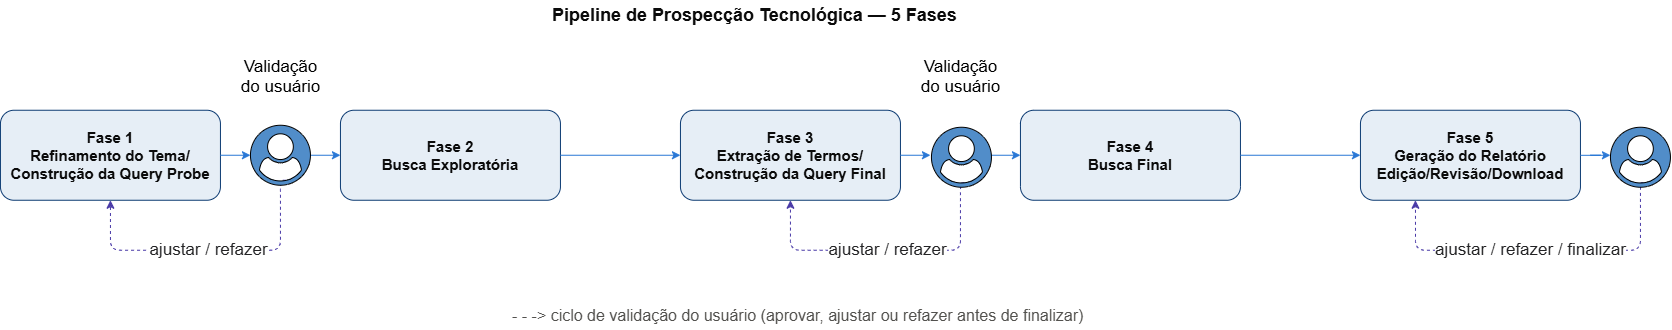
\includegraphics[width=0.9\textwidth]{img/pipeline_cinco_fases.png}
    \caption{Visão geral das cinco fases do \textit{pipeline} de prospecção tecnológica.}
    \label{fig:pipeline-cinco-fases}
\end{figure}

  \subsection{Fase 1: Refinamento do Tema}

  A primeira fase recebe o tema bruto fornecido pelo usuário e o processa por
meio do modelo de LLM remota, que analisa o texto de
entrada e gera um conjunto expandido de variações temáticas relacionadas ao tema,
abrangendo sinônimos, termos técnicos correlatos e variações terminológicas em
inglês --- idioma predominante nas bases de patentes e artigos científicos. O
resultado é apresentado ao usuário para validação, que pode aprovar a variação
gerada, solicitar maior especificidade ou alterá-la diretamente.

  O \textit{prompt} utilizado nesta fase segue as diretrizes de
\textit{prompt engineering} descritas na Seção~2.4, em particular o padrão de
definição de papel (\textit{persona pattern}) e o uso de exemplos contrastantes
bom/ruim \cite{white2023}, instruindo
explicitamente o modelo a gerar variações técnicas e organizadas em ordem decrescente de relevância para o tema informado. A
temperatura de inferência é mantida em $0{,}3$ para privilegiar respostas
consistentes \cite{zhao2023}.

  \subsection{Fase 2: Busca Exploratória}

  Com o tema validado, o sistema constrói consultas específicas para cada
API --- CQL para o OPS e a sintaxe própria para o Scopus e Lens --- e realiza buscas
exploratórias em paralelo nas bases de artigos e patentes, limitadas a 10 resultados iniciais
por API. O objetivo desta fase é recuperar uma amostra representativa de
documentos que permita, na fase seguinte, identificar os termos mais
relevantes e recorrentes no domínio pesquisado \cite{porter2004}. A duração
típica é de 10 a 20 segundos.

  Antes de cada consulta ser efetivamente enviada às APIs externas, sua
complexidade estrutural é avaliada por um componente determinístico que conta
operadores booleanos, profundidade de aninhamento de parênteses e número de
termos, comparando o escore resultante contra um limiar configurável; caso o
limiar seja excedido, o sistema solicita uma nova tentativa ao LLM, reinjetando
no \textit{prompt} o resultado exato da avaliação anterior (padrão de
autocorreção por métrica determinística descrito na Seção~2.4), até um número
máximo de tentativas --- após o qual a tentativa menos complexa gerada é
utilizada, com aviso ao usuário. Esse mecanismo existe porque consultas mais
"abrangentes", com muitos termos e operadores aninhados, tendem, na prática, a
quebrar o analisador sintático das APIs remotas ou retornar erro/zero
resultados, e não necessariamente mais resultados.

%% TODO (imagem pendente): diagrama do loop de retentativa por complexidade
%% (consulta -> análise de complexidade -> excede limiar? -> sufixo de
%% simplificação -> nova tentativa -> melhor-de-N).
% \begin{figure}[H]
%     \centering
%     
\includegraphics[width=0.85\textwidth]{img/loop_retentativa_complexidade.png}
%     \caption{Ciclo de verificação de complexidade e retentativa assistida por LLM.}
%     \label{fig:loop-complexidade}
% \end{figure}

  Os construtores de consulta (\textit{query builders}) são responsáveis por transformar os termos validados
em consultas booleanas estruturadas utilizando dicionários próprios de cada API. Por exemplo, o construtor para o OPS gera consultas
CQL com operadores \texttt{AND}, \texttt{OR} e \texttt{NOT}, com filtros por
campo (\texttt{ti} para título, \texttt{ab} para resumo, \texttt{pa} para
depositante) e por ano de publicação. Já o construtor para o Scopus converte os
termos em uma sintaxe compatível com a API da Elsevier, utilizando campos como
\texttt{TITLE}, \texttt{ABS} e \texttt{KEY}, também com suporte a operadores lógicos e
filtros temporais. Todos os construtores compartilham o mesmo contrato de
entrada e saída, o que os torna substituíveis entre si pelo serviço de
orquestração, conforme discutido na Seção~\ref{sec:hexagonal} à luz do
Princípio da Substituição de Liskov.

  Os documentos recuperados nesta fase, antes de seguirem para a extração de
termos (Seção~\ref{sec:extracao-termos}), passam ainda pelo filtro de idioma e
pelo filtro de relevância documento-tema descritos na
Seção~\ref{sec:filtragem-documentos} --- é esse último filtro, e não um
critério definido diretamente pela API de busca, que determina o subconjunto
efetivo de documentos que alimentará a extração de termos.

  \subsection{Fase 3: Extração de Termos}
  \label{sec:extracao-termos}

  Os resultados da busca exploratória de cada tipo de base são processados por um pipeline
local de PLN --- e não por uma nova chamada ao LLM ---, responsável por extrair,
pontuar e ranquear os termos mais relevantes a partir de título e resumo de
cada documento recuperado. Diferentemente da função de complexidade de
consulta (Seção~\ref{sec:complexidade}), que é uma métrica original criada
pelos autores, o pipeline de extração de termos combina métodos consagrados na
literatura de recuperação de informação (PatternRank, BM25F, KeyBERT, RRF e
C-value, Seção~\ref{sec:filtragem-documentos}), organizados por uma sequência
de filtros --- estes sim, decisões de projeto específicas deste trabalho ---
detalhada passo a passo a seguir.

  \begin{enumerate}[label=\textbf{Passo \arabic*.}, leftmargin=2.2cm]

    \item \textbf{Limpeza e delimitação do texto.} Título e resumo de cada
    documento são convertidos para minúsculas, com remoção de URLs e
    substituição de hífens por espaços, e mantidos alinhados por documento
    (o BM25F exige saber qual título pertence a qual resumo). Vírgulas e
    pontos e vírgulas são convertidos em pontos, e todo texto recebe
    pontuação final: sem essas fronteiras explícitas, o padrão gramatical do
    passo seguinte "vaza" do fim de um título para o início do próximo, ou
    entre itens de uma lista, produzindo candidatos que não existem em
    nenhum dos textos originais.

    \item \textbf{Geração de candidatos (PatternRank).} Sobre o conjunto de
    textos, são extraídas as frases nominais maximais que obedecem ao padrão
    gramatical \textit{adjetivo* substantivo+} \cite{schopf2022}, com até
    cinco palavras. Cada candidato já é uma expressão gramaticalmente
    completa, e não uma janela arbitrária de palavras.

    \item \textbf{Filtro de termos originais.} São removidos os unigramas
    idênticos aos termos já informados pelo usuário no tema e na descrição;
    expressões de duas ou mais palavras são mantidas, ainda que contenham um
    termo original, por acrescentarem especificidade.

    \item \textbf{Filtro de qualidade lexical.} Palavras de uma lista de cerca
    de 55 palavras de fronteira lexical (\textit{a, an, the, of, is, are,
    this, that, high, low, new, such, about}) são removidas repetidamente das
    extremidades do candidato (\textit{"the good permeability"}
    $\rightarrow$ \textit{"good permeability"} $\rightarrow$
    \textit{"permeability"}), em vez de o candidato inteiro ser descartado; o
    candidato é descartado se qualquer palavra restante pertencer a uma lista
    de termos estruturais típicos de patentes (\textit{wherein, comprising,
    said, first, second, configured, plurality, substantially, device}) ou
    de texto acadêmico (\textit{proposed, novel, improved, significant,
    method, technique, framework, model, system, based, compared}).
    Candidatos que convergem para a mesma forma após o corte são
    deduplicados.

    \item \textbf{Canal léxico (BM25F).} Para cada candidato $t$ e documento
    $d$, a frequência do candidato em cada campo é normalizada pelo tamanho
    do campo e ponderada pelo peso do campo --- 3 para o título e 1 para o
    resumo, premissa de que termos presentes no título são, em média, mais
    representativos do conteúdo do documento \cite{robertson2004}:
    $$
    \tilde{f}_{t,d} = w_{\text{tít}} \frac{f_{t,d}^{\text{tít}}}{B_{d}^{\text{tít}}} + w_{\text{res}} \frac{f_{t,d}^{\text{res}}}{B_{d}^{\text{res}}}, \qquad B_{d}^{c} = (1 - b) + b \frac{|d^{c}|}{\overline{|d^{c}|}},
    $$
    e o escore agregado sobre os $N$ documentos, dos quais $n_t$ contêm o
    candidato, é
    $$
    \text{BM25F}(t) = \sum_{d} \frac{\tilde{f}_{t,d}}{k_1 + \tilde{f}_{t,d}} \cdot \ln\left(1 + \frac{N - n_t + 0{,}5}{n_t + 0{,}5}\right),
    $$
    com $k_1 = 1{,}2$ e $b = 0{,}75$, valores usuais na literatura
    \cite{robertson2009}.

    \item \textbf{Canal semântico (KeyBERT).} Cada candidato e o texto do
    conjunto de documentos são convertidos em \textit{embeddings} de
    sentença, e o escore do candidato é a similaridade de cosseno entre os
    dois vetores \cite{grootendorst2020, reimers2019}.

    \item \textbf{Primeira fusão (saliência).} Os dois canais são combinados
    por RRF \cite{cormack2009}, com $k = 60$:
    $\text{saliência}(t) = \frac{1}{60 + \text{pos}_{\text{BM25F}}(t)} +
    \frac{1}{60 + \text{pos}_{\text{KeyBERT}}(t)}$.

    \item \textbf{Qualidade estrutural.} Cada candidato recebe um escore de
    qualidade estrutural: $-0{,}4$ para unigramas (palavras isoladas tendem a
    ser pouco informativas), $0$ para bigramas e $+0{,}25$ para trigramas ou
    maiores (tendem a capturar conceitos técnicos completos, como
    \textit{"convolutional neural network"}), acrescido de $-0{,}8$ quando a
    sequência de classes gramaticais do candidato corresponde a um padrão
    catalogado como pouco informativo --- por exemplo, dois verbos
    consecutivos ou a sequência advérbio-verbo-substantivo.

    \item \textbf{Segunda fusão (escore final).} Saliência e qualidade
    estrutural são novamente combinadas por RRF, produzindo o escore final
    do candidato. Como ambas as fusões operam sobre posições, e não sobre
    escores, nenhum peso precisa ser calibrado entre escalas diferentes.

    \item \textbf{Redundância entre termos aninhados (C-value).} Para cada
    candidato $a$, com $|a|$ palavras e frequência $f(a)$, sendo $T_a$ o
    conjunto de candidatos mais longos que o contêm de forma contígua,
    calcula-se \cite{frantzi2000}
    $$
    \text{C-value}(a) =
    \begin{cases}
      \log_2 |a| \cdot f(a), & \text{se } T_a = \emptyset, \\[4pt]
      \log_2 |a| \cdot \left( f(a) - \dfrac{1}{|T_a|} \displaystyle\sum_{b \in T_a} f(b) \right), & \text{caso contrário},
    \end{cases}
    $$
    (com $|a|$ limitado inferiormente a 2, para que unigramas não recebam
    $\log_2 1 = 0$). Candidatos com C-value não positivo --- que ocorrem
    apenas como parte de expressões mais longas, sem uso independente --- são
    descartados. Em seguida, entre os remanescentes ranqueados pelo escore
    final, um candidato contido de forma contígua em outro já mantido, de
    posição superior, é descartado: entre \textit{"ultrafiltration
    membrane"} e \textit{"composite ultrafiltration membrane"}, apenas o de
    maior escore permanece. Esse passo substitui um filtro anterior de
    sobreposição de palavras e, antes dele, um mecanismo de Relevância
    Marginal Máxima (\textit{Maximal Marginal Relevance}, MMR) descartado
    por apresentar custo cúbico no número de candidatos.

    \item \textbf{Limiar e corte final.} São mantidos os candidatos com
    escore final igual ou superior a $0{,}024$ --- limiar calibrado para a
    escala do RRF, cujos valores ficam, com $k = 60$, aproximadamente entre
    $0{,}018$ e $0{,}033$ ---, completados, se necessário, pelos melhores
    candidatos abaixo do limiar até um mínimo de 10 termos, e limitados a no
    máximo 60 termos, já ordenados pelo escore final.

  \end{enumerate}

  O pipeline descrito substituiu uma primeira versão, na qual os candidatos
eram sub-n-gramas de uma a três palavras extraídos de \textit{noun chunks} do
spaCy e o escore era uma combinação linear fixa de TF-IDF
\cite{saltonbuckley1988} e KeyBERT ($0{,}6 \times \text{TF-IDF} + 0{,}4 \times
\text{KeyBERT}$), calculada separadamente para título e resumo. Em uma
comparação direta sobre os mesmos conjuntos de documentos de dez domínios
tecnológicos distintos (de dessalinização a biossensores), a versão atual foi
cerca de 3,6 vezes mais rápida (37,3~s contra 10,4~s no total) --- o KeyBERT
passou a ser chamado uma única vez por requisição, e o conjunto de candidatos
brutos caiu de até 182 para cerca de 50 --- e obteve nota média de qualidade,
atribuída pelos autores aos termos retornados, de 8,1 contra 5,7, sem nenhum
domínio avaliado como pior. O ganho mais visível foi o fim do truncamento
sistemático em três palavras, presente em nove dos dez casos da versão
anterior: expressões corretas de quatro ou cinco palavras passaram a ser
extraídas. Em contrapartida, a fusão por posições penaliza unigramas
frequentes com menos força que a penalidade aditiva anterior, admitindo de
dois a quatro unigramas fracos a mais por caso em domínios com palavras de alta
frequência, e o padrão gramatical adotado não cobre gerúndios modificadores
(como em \textit{"privacy preserving"}). O limiar de $0{,}024$ foi calibrado
sobre esse conjunto de teste e deve ser revisto à medida que houver histórico
real de seleção de termos pelos usuários.

%% TODO (imagem pendente): fluxograma do pipeline de extração de termos,
%% seguindo os onze passos acima (limpeza -> PatternRank -> filtros ->
%% BM25F / KeyBERT -> RRF 1 -> qualidade estrutural -> RRF 2 -> C-value ->
%% aninhamento -> limiar/corte).
% \begin{figure}[H]
%     \centering
%     
\includegraphics[width=0.9\textwidth]{img/pipeline_extracao_termos.png}
%     \caption{Fluxograma dos onze passos do pipeline de extração e pontuação de termos.}
%     \label{fig:pipeline-extracao-termos}
% \end{figure}

  \paragraph{Exemplo numérico de cálculo.} Para ilustrar a aplicação conjunta
dos Passos 7 a 11, considere dois candidatos extraídos de um conjunto de
documentos sobre veículos autônomos: o trigrama \textit{"autonomous vehicle
navigation"}, 2.º colocado no canal BM25F e 1.º no KeyBERT, e o unigrama
\textit{"vehicle"}, 1.º no BM25F (por ser muito frequente) e apenas 9.º no
KeyBERT. Aplicando o Passo 7:

$$
\text{saliência}(\text{autonomous vehicle navigation}) = \frac{1}{60 + 2} + \frac{1}{60 + 1} = 0{,}01613 + 0{,}01639 = 0{,}03252
$$
$$
\text{saliência}(\text{vehicle}) = \frac{1}{60 + 1} + \frac{1}{60 + 9} = 0{,}01639 + 0{,}01449 = 0{,}03088
$$

  O trigrama, portanto, ocupa a 1.ª posição de saliência e o unigrama, a
2.ª: estar bem posicionado nos dois canais supera ser o primeiro em apenas
um. No Passo 8, o trigrama recebe $+0{,}25$ de qualidade estrutural e o
unigrama, $-0{,}4$; supondo que, no \textit{ranking} de qualidade estrutural do
lote, o trigrama ocupe a 3.ª posição e o unigrama a 40.ª, o Passo 9 resulta em

$$
\text{final}(\text{autonomous vehicle navigation}) = \frac{1}{60 + 1} + \frac{1}{60 + 3} = 0{,}01639 + 0{,}01587 = 0{,}03226
$$
$$
\text{final}(\text{vehicle}) = \frac{1}{60 + 2} + \frac{1}{60 + 40} = 0{,}01613 + 0{,}01000 = 0{,}02613
$$

  Ambos superam o limiar de $0{,}024$ (Passo 11), mas com uma margem bem
maior para o trigrama, mais específico. Se o lote contivesse também
\textit{"vehicle navigation"}, com escore final inferior ao de
\textit{"autonomous vehicle navigation"}, ele seria descartado no Passo 10,
por estar contido de forma contígua em um termo de posição superior.

  A lista ranqueada resultante é apresentada ao
usuário com indicação de relevância, junto da escolha, por fonte, do nível de
abrangência desejado para a consulta final (específica, balanceada ou ampla) ---
sendo a diferença entre esses três níveis, na prática, o limiar mínimo de
escore utilizado para selecionar quais dos termos marcados pelo usuário são
oferecidos ao LLM como contexto na fase seguinte. Como o escore final do RRF
vive em uma faixa estreita, ele é antes normalizado para o intervalo $[0, 1]$
(normalização mín--máx sobre os termos selecionados), e os limiares são
aplicados sobre esse valor: 0,4 para a variante específica, 0,3 para a
balanceada e 0,2 para a ampla. Quanto mais específica a variante, maior o
limiar e menor o conjunto de termos considerado. Esta fase é crítica para a qualidade
dos resultados finais, pois as consultas construídas a partir de termos
extraídos dos próprios documentos recuperados tendem a ser mais específicas e
representativas do universo em questão --- patentes ou artigos --- do que
aquelas baseadas apenas nos termos inicialmente fornecidos pelo usuário
\cite{porter2004}.

  \subsection{Fase 4: Busca Final}

  Com os termos selecionados pelo usuário, o modelo de LLM remoto gera a
variante de consulta final escolhida, seguindo o mesmo mecanismo de
verificação de complexidade e retentativa descrito na Fase~2; o sistema
reconstrói as consultas utilizando os construtores de consulta,
combinando os termos em estruturas booleanas otimizadas, e executa a busca final
em ambas as APIs. Os resultados são consolidados com remoção de duplicatas, gerando o conjunto definitivo de patentes
e artigos que fundamentará a análise.

  Nesta fase, aplica-se particular atenção à construção de consultas que não
excedam os limites de complexidade aceitos pelas APIs. Consultas com número
excessivo de termos encadeados por operadores \texttt{OR} podem ser rejeitadas
ou truncadas, o que exige uma estratégia de particionamento e combinação de
resultados implementada no serviço de busca.

  Três decisões de robustez da busca final têm impacto direto sobre a
fidelidade dos indicadores do relatório. Primeiro, o sistema distingue o
\textbf{total real} de documentos informado pela base para a consulta --- ou,
quando a base não o informa, a soma das contagens por ano --- da
\textbf{amostra} efetivamente baixada e analisada: o total real é o que aparece
no quadro de busca do relatório, e a amostra, o que fundamenta as análises.
Segundo, na contagem de artigos por ano, base da curva~S científica, falhas de
rede são repetidas automaticamente e, persistindo, o ano afetado é
\textbf{omitido} da série, e nunca registrado como zero --- um zero falso criaria
um "vale" artificial que distorceria o ajuste logístico. Terceiro, nomes de
depositantes em escrita não latina (chinês, japonês, coreano) são substituídos
pela forma latinizada fornecida pela própria API OPS, já que o compilador
LaTeX descarta esses caracteres e o depositante apareceria em branco nos
gráficos e no texto.

  \subsection{Fase 5: Geração do Relatório}
  \label{sec:fase5}

  A última fase transforma os documentos da busca final em um relatório no
padrão REPTEC/AGITEC \cite{agitec2024, reptec2023tetra}, editável e
compilável em PDF. Ela é organizada em cinco etapas: consolidação e gráficos,
redação das seções, montagem do documento, revisão e exportação.

    \subsubsection{Consolidação e gráficos}

  O módulo de consolidação agrega os documentos coletados por ano, por
depositante e por classificação CPC para as patentes, e por ano, por
instituição e por área de estudo para os artigos, ajusta as curvas~S de
patentes e de artigos e calcula os pontos GP/MP/SP com seu diagnóstico de
confiabilidade (Seção~\ref{sec:curva-s}). Somente as figuras previstas no
padrão REPTEC são geradas: histórico anual de patentes e de artigos,
principais depositantes e instituições, quadros com as dez classificações CPC
e as dez áreas de estudo mais frequentes e as duas curvas~S. As séries
consideram apenas anos completos, as classificações IPC são tratadas como CPC
e descritas pelos títulos oficiais da classificação, e nomes com mais de 45
caracteres são abreviados. O título de cada figura não é desenhado na
imagem, mas escrito na legenda LaTeX, seguida da indicação "Fonte: O autor.",
como no relatório de referência. Cada gráfico é armazenado no MinIO junto de
seu resumo numérico, e é esse resumo --- e não a imagem --- que o modelo de
linguagem recebe para descrever a figura.

    \subsubsection{Redação das seções}

  Nem toda seção do relatório passa pelo modelo de linguagem. A estrutura,
extraída de um REPTEC real \cite{reptec2023tetra}, separa o que depende dos
dados da busca do que é essencialmente igual em todo relatório, como resume a
Tabela~\ref{tab:secoes-relatorio}.

\begin{table}[H]
\centering
\caption{Seções do relatório e forma de produção}
\label{tab:secoes-relatorio}
\begin{tabular}{p{5.0cm}p{8.2cm}}
\toprule
\textbf{Seção} & \textbf{Como é produzida} \\
\midrule
Capa e sumário & \textit{Template} LaTeX \\
1 Finalidade & Texto fixo, interpolando o tema e o destinatário informados \\
2 Referências & Documentos administrativos informados pelo usuário (DIEx, ofícios) \\
3 Objetivo & Texto informado pelo usuário \\
4 Introdução & LLM, com contexto do RAG \\
5 Metodologia (5.1 a 5.4) & Texto fixo com as figuras de referência sobre curva~S \cite{madeo2019, kucharavy2011}, descrição genérica do apoio computacional e interpolação das palavras-chave, do período e das bases consultadas \\
6 Resultados (6.1 Científicas, 6.2 Tecnológicas, 6.3 Tendências e Ciclo de Vida) & LLM, uma chamada por subseção, com contexto do RAG e resumos numéricos dos gráficos; a 6.2 inclui o quadro com as consultas de busca e o total real de documentos \\
7 Conclusão & LLM, com estrutura orientada (estágio do ciclo de vida, destaques e recomendação) \\
8 Referências bibliográficas & Bibliografia fixa da Metodologia, obras efetivamente citadas no texto e obras adicionadas pelo usuário \\
Local, data e assinaturas & Formulário (nome, posto/graduação e função de quem elabora, revisa e aprova) \\
\bottomrule
\end{tabular}
\end{table}

  Cada seção redigida por LLM passa por duas requisições separadas: a
primeira indexa os documentos da sessão, se ainda não indexados, e recupera e
persiste o contexto da seção (Seção~\ref{sec:rag}); a segunda monta o
\textit{prompt} com esse contexto, chama o modelo e persiste o texto. Essa
divisão permite à interface mostrar o andamento seção a seção e mantém cada
chamada ao modelo restrita ao contexto de uma única seção, o que é relevante
para modelos locais de janela de contexto pequena.

  O \textit{prompt} de sistema impõe texto impessoal e proíbe expressões que
revelam o funcionamento interno do sistema (escores de relevância, "N/A",
"no contexto fornecido"). Em torno do modelo, módulos determinísticos
garantem o que não pode depender dele:

  \begin{itemize}
    \item \textbf{Figuras no contexto.} O modelo é instruído a seguir o padrão
    do relatório de referência --- apresentar a figura, exibi-la e, em seguida,
    interpretar seus números --- escrevendo marcadores para a referência e
    para a posição de cada figura. Um pós-processador converte os marcadores
    em comandos LaTeX; se o modelo cita uma figura sem posicioná-la, ela é
    inserida logo após o parágrafo que a cita, e figuras não citadas vão para
    o fim da seção, na ordem do relatório de referência. O mesmo
    pós-processador corrige "Figura" e "Quadro" conforme o tipo do elemento,
    ajustando a concordância do artigo ("a Figura", "o Quadro").
    \item \textbf{Ciclo de vida calculado.} O estágio da tecnologia
    (emergente, crescimento, maturidade ou saturação) é calculado a partir de
    GP, MP e SP e entregue ao modelo como fato, e não inferido por ele.
    \item \textbf{Citações rastreáveis.} Só são aceitas citações no formato
    "(SOBRENOME et al., ano)" que correspondam a documentos recuperados pelo
    RAG; citações inventadas são removidas do texto, autores homônimos
    recebem sufixo de letra (2020a, 2020b), e as referências ABNT das obras
    efetivamente citadas são acrescentadas à seção de referências.
    \item \textbf{Validação do texto.} Números são convertidos para o padrão
    brasileiro (17,3\%; 1.800) e o texto é inspecionado em busca de vestígios
    do \textit{pipeline}; se algum for encontrado, a seção é regenerada uma vez
    com instrução de correção e, persistindo o problema, a geração falha com
    mensagem explícita, em vez de produzir um texto defeituoso.
  \end{itemize}

    \subsubsection{Montagem do documento}

  A montagem reúne as seções persistidas e as imagens já armazenadas no
MinIO --- sem disparar nenhuma nova geração --- e renderiza o \textit{template}
LaTeX, que reproduz a formatação do relatório de referência: cabeçalho com o
número do relatório e o tema, rodapé "Página $x$ de $y$", títulos de seção em
negrito e caixa alta, texto justificado com recuo de parágrafo, espaçamento
de 1,5, figuras e quadros numerados com legenda e fonte, e bloco de
assinaturas no formato "NOME -- POSTO", com a função na linha seguinte. O
\texttt{.tex} resultante é armazenado no MinIO junto de uma cópia de
referência, usada depois pela revisão para identificar o que o usuário
editou. A compilação em PDF é uma ação separada, sempre disparada pelo
usuário, executada pelo serviço TeX Live dedicado; uma falha de compilação não
apaga o \texttt{.tex} já montado.

    \subsubsection{Edição e revisão}

  O \texttt{.tex} é aberto em um editor na própria interface, com um painel
lateral de imagens --- as geradas pelo sistema, as figuras fixas e as
anexadas pelo usuário --- a partir do qual cada imagem pode ser inserida no
documento, aberta, baixada ou, no caso dos anexos, excluída. A revisão do
documento combina três verificações:

  \begin{enumerate}[label=(\alph*)]
    \item \textbf{Verificação de LaTeX}: chaves e ambientes desbalanceados,
    referências a rótulos ou imagens inexistentes, caracteres especiais sem
    escape e erros do último registro de compilação.
    \item \textbf{LanguageTool}: ortografia, acentuação, concordância e
    gramática, aplicados apenas às seções geradas por LLM e às linhas
    editadas pelo usuário --- identificadas pela comparação com a cópia de
    referência da montagem ---, de modo que o texto fixo, já revisado, não é
    reprocessado. Os comandos LaTeX são enviados como marcação, e não como
    texto, para não gerarem falsos positivos.
    \item \textbf{Revisão por LLM (opcional)}: uma segunda opinião, com ponto
    de uso de LLM próprio --- o que permite empregar um modelo melhor em
    português que o da redação ---, restrita a concordância, acentuação e
    ortografia. Uma sugestão só é aceita se o trecho original existir
    literalmente no texto e se a correção não alterar números, citações ou
    comandos LaTeX.
  \end{enumerate}

  As sugestões são apresentadas por seção, e o usuário aplica ou ignora cada
uma individualmente.

    \subsubsection{Exportação}

  Além do PDF, o sistema exporta um pacote \texttt{.zip} com o \texttt{.tex} e
todas as imagens nele referenciadas, nomeado segundo o número e o ano do
relatório, o que permite ao usuário continuar a edição em qualquer ambiente
LaTeX, como o Overleaf.


% ------------------------------------------------------------
%  CRONOGRAMA
% ------------------------------------------------------------
  \section{Cronograma}

  O cronograma do projeto foi estruturado em três fases, alinhadas com as datas
de entrega dos relatórios parcial e final, conforme apresentado na
Figura~\ref{fig:cronograma}.

\begin{figure}[H]
    \centering
    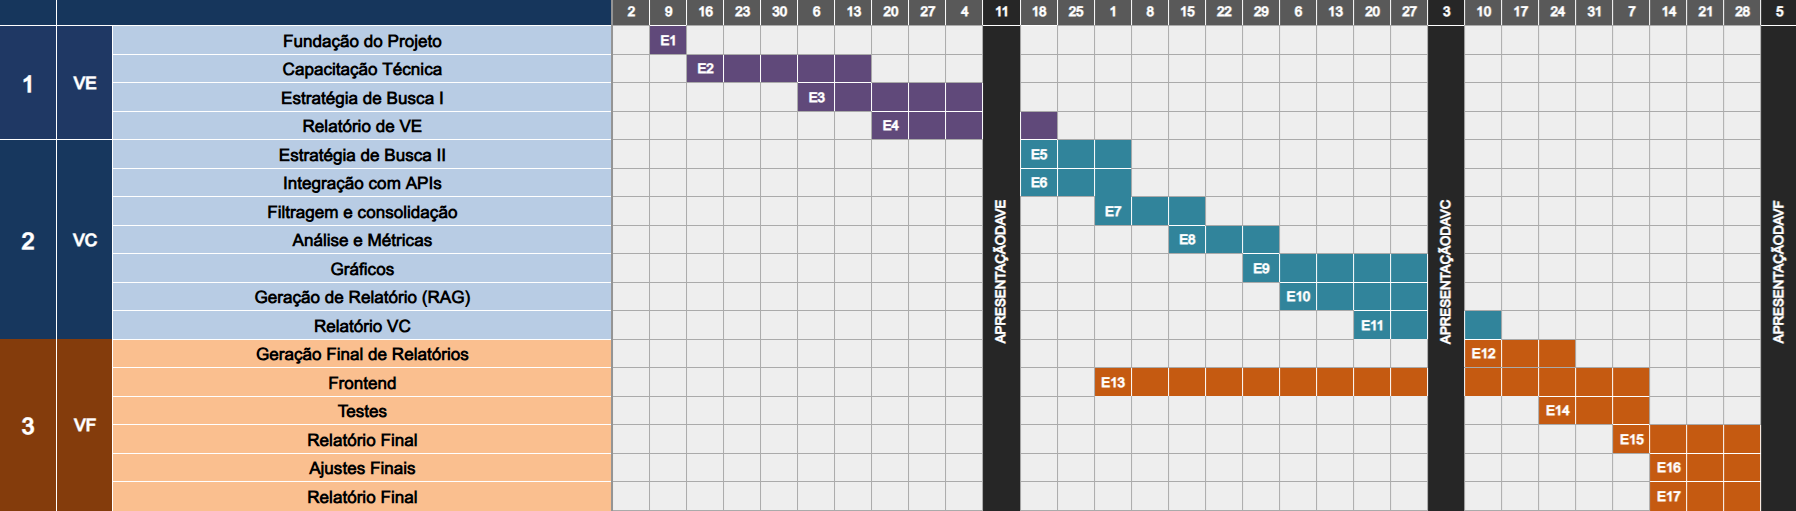
\includegraphics[width=1.1\textwidth]{img/cronograma.png}
    \caption{Cronograma de desenvolvimento do projeto.}
    \label{fig:cronograma}
\end{figure}
   
  O cronograma do projeto foi estruturado em três fases, identificadas como VE,
VC e VF, alinhadas com as datas de entrega dos relatórios parcial e final,
conforme apresentado na Figura~\ref{fig:cronograma}. Cada fase agrupa um
conjunto de atividades sequenciais e interdependentes, identificadas pelos
marcos E1 a E17.

    \subsection{Fase 1 --- VE}

  A primeira fase cobre as atividades de fundação, capacitação e planejamento
inicial do sistema. A atividade \textbf{E1 --- Fundação do Projeto} compreende
o levantamento de requisitos junto aos \textit{stakeholders} da AGITEC
\cite{agitec2024}, a definição do problema e dos objetivos do sistema, o estudo
do padrão de relatório REPTEC/AGITEC --- incluindo o exemplo real disponibilizado
em \cite{reptec2023tetra} --- e a concepção inicial do
\textit{pipeline}, produzindo como resultado um documento de requisitos e o
escopo do sistema.

  A atividade \textbf{E2 --- Capacitação Técnica} é dedicada ao aprofundamento
nos fundamentos que sustentam o sistema: LLMs e modelos de geração de texto
\cite{zhao2023, brown2020}, técnicas de \textit{embedding} semântico
\cite{reimers2019, mikolov2013}, ferramentas de PLN (Natural Language Processing), RAG e bancos de dados
vetoriais \cite{lewis2020, gao2024}, arquitetura hexagonal e princípios SOLID
\cite{cockburn2005, martin2002, martin2017}, bem como o estudo das APIs de busca
em patentes e artigos científicos disponíveis para integração. O resultado
desta atividade é a fundamentação teórica consolidada, base do presente
relatório.

  A atividade \textbf{E3 --- Estratégia de Busca~I} tem como objetivo definir
a estratégia de busca do sistema, abrangendo a estrutura das consultas por
campos (título, resumo), o uso de operadores booleanos e a distinção entre
busca exploratória e busca final. O resultado é a primeira versão funcional
do \textit{pipeline} de busca. Por fim, a atividade \textbf{E4 --- Relatório de VE} corresponde à elaboração do presente relatório parcial, contendo introdução, fundamentação teórica, solução proposta com especificação de requisitos e arquitetura do sistema, descrição do \textit{pipeline} e protótipo inicial, e considerações parciais.

    \subsection{Fase 2 --- VC}

  A segunda fase é dedicada à implementação completa do \textit{pipeline} de
prospecção tecnológica. A atividade \textbf{E5 --- Estratégia de Busca~II}
dá continuidade à fase anterior, com a implementação da expansão semântica
dos termos por LLM e do \textit{query builder} inicial, produzindo uma
consulta funcional para as APIs.

  A atividade \textbf{E6 --- Integração com APIs} implementa as conexões com
as APIs de busca de patentes e artigos científicos, incluindo o tratamento
de respostas, a paginação e o controle dos limites de requisição. O
resultado é o sistema retornando dados reais a partir de consultas estruturadas.

  A atividade \textbf{E7 --- Filtragem e Consolidação} trata os metadados
recuperados, com remoção de duplicatas, normalização dos dados provenientes
de diferentes fontes e estruturação no banco de dados relacional (entidades
de sessão de pesquisa, patente e artigo).

Na sequência, a
atividade \textbf{E8 --- Análise e Métricas} realiza as agregações por ano,
por autores e por instituições, o levantamento dos principais depositantes
e periódicos, as métricas de citação e o cálculo da curva~S
\cite{foster1986, fisherpry1971, rogers2003}, incluindo a implementação do
estimador de completude amostral Chao1 \cite{chao1984} e da verificação de
estabilidade de \textit{ranking} por \textit{bootstrap} \cite{efron1979}
(Seção~\ref{sec:chao1bootstrap}) sobre os agregados de classificação
tecnológica, área de estudo e depositante/instituição.

  A atividade \textbf{E9 --- Gráficos} implementa a geração automática de
todas as visualizações necessárias ao relatório: curva~S com pontos GP/MP/SP e
diagnóstico de confiabilidade, evolução temporal,
distribuições por classificação tecnológica e por área de estudo, entre
outros. A atividade \textbf{E10 --- Geração de Relatório (RAG)} implementa
o \textit{pipeline} completo de geração automática do relatório, integrando
o módulo de consolidação de dados, o subsistema RAG local com ChromaDB e
\textit{embeddings} \cite{lewis2020, gao2024} e o modelo de linguagem local,
produzindo o relatório em LaTeX no padrão REPTEC/AGITEC \cite{agitec2024, reptec2023tetra},
e inclui a integração inicial do armazenamento de objetos MinIO para
persistência dos gráficos e do relatório gerado.

A fase~2 encerra-se com a atividade \textbf{E11 --- Relatório VC}, contendo a descrição detalhada do \textit{pipeline} implementado, a arquitetura consolidada do sistema, os resultados preliminares das buscas realizadas e a análise inicial dos dados recuperados, incluindo métricas e gráficos gerados.

    \subsection{Fase 3 --- VF}

  A terceira fase é voltada ao refinamento, validação e entrega final do
sistema. A atividade \textbf{E12 --- Geração Final de Relatórios} executa
casos reais de prospecção, gera relatórios completos e ajusta a qualidade
textual das seções geradas pelo LLM, mitigando possíveis alucinações
\cite{ji2022}.

  A atividade \textbf{E13 --- Frontend} conclui a interface \textit{web},
com a implementação da etapa de edição e exportação do relatório final e
integração completa com o \textit{backend}, permitindo que o usuário acompanhe o progresso do \textit{pipeline}, edite
o relatório gerado e exporte o documento final. A atividade
\textbf{E14 --- Testes} realiza casos de teste com temas reais, valida os
relatórios gerados e promove os ajustes finais de qualidade.

  As atividades \textbf{E15 --- Relatório Final} e \textbf{E16 --- Ajustes
Finais} cobrem, respectivamente, a escrita do relatório final completo
(resultados, discussão, conclusão e trabalhos futuros) e a implementação
das correções indicadas pela banca e pelo orientador --- incluindo, se ainda
pendente, a conclusão da integração do MinIO com a instância remota do
Exército --- bem como a revisão
geral do sistema. A fase encerra-se com a atividade \textbf{E17}, que realiza a conferência final com os requisitos levantados na VE, a validação do \textit{checklist} de completude do sistema e a entrega do relatório final completo acompanhado do sistema em sua versão definitiva.

    \subsection{Relação de Entregáveis}

  Os principais entregáveis previstos em cada fase são os seguintes:

  \textbf{VE (E1--E4):} documento de requisitos e escopo do sistema;
fundamentação teórica; primeira versão do \textit{pipeline} de busca;
relatório parcial da VE; apresentação.

  \textbf{VC (E5--E11):} \textit{query builder} e integração funcional com
as APIs de busca; módulos de filtragem, consolidação e análise de metadados;
geração automática de gráficos e curva~S com GP/MP/SP; \textit{pipeline} RAG local completo
com geração de relatório em LaTeX; integração inicial do MinIO; relatório parcial da VC; apresentação.

  \textbf{VF (E12--E17):} relatórios finais gerados a partir de casos reais;
interface \textit{web} completa com editor e exportação; integração MinIO
concluída; suite de testes validados;
ajustes pós-banca; relatório final; apresentação.

% ============================================================
%  CAPÍTULO 6 — CONSIDERAÇÕES FINAIS
% ============================================================
\section{Considerações Finais}

  \subsection{Resultados Esperados}

  Ao final do desenvolvimento, espera-se que o sistema seja capaz de reduzir
significativamente o tempo necessário para a realização de um levantamento
completo de prospecção tecnológica \cite{porter2004, mayerhoff2008} --- de dias de trabalho manual a horas ou até mesmo minutos de processamento automatizado. Essa redução tem impacto direto na
disponibilidade de tempo dos técnicos e engenheiros envolvidos em projetos de
PD\&I do Exército Brasileiro para atividades de maior valor estratégico.

  Além disso, espera-se que os relatórios gerados automaticamente apresentem
estrutura, coerência e embasamento factual adequados ao padrão REPTEC/AGITEC
\cite{agitec2024}, servindo como ponto de partida para análises mais aprofundadas
pelos especialistas responsáveis por cada projeto. A viabilidade metodológica do
formalismo GP/MP/SP adotado para leitura da curva~S, em particular, já está
demonstrada na prática institucional da AGITEC com dados reais de patentes e
publicações, como evidenciado em \cite{reptec2023tetra}, o que reforça a
adequação do método escolhido para a automação proposta. É importante ressaltar que
o sistema não substitui o julgamento especializado do analista humano, mas
fornece um documento estruturado e rastreável que torna esse julgamento mais
eficiente e informado --- premissa que reflete o papel da IA como ferramenta de
apoio à decisão, e não como substituto do especialista \cite{lewis2020, ji2022}.

  \subsection{Limitações}

  O sistema apresenta algumas limitações que devem ser consideradas. Os
modelos de linguagem locais testados (Qwen~2.5~(3B) e Gemma~3~(4B))
\cite{zhao2023}, embora adequados ao contexto local, possuem capacidade
inferior à de modelos maiores \cite{brown2020}, com impacto observado na
qualidade do português formal gerado --- sobretudo na concordância verbal com
sujeito distante --- e na profundidade das análises; a etapa de revisão
(Seção~\ref{sec:fase5}) detecta boa parte desses erros, mas não substitui a
leitura do especialista, e a qualidade do texto deverá ser reavaliada com o LLM
disponibilizado na intranet do Exército, ainda não testado. O corpus do RAG é
composto apenas por título e resumo dos documentos da busca final, e, como os
resumos de artigos nem sempre são devolvidos pelas APIs, tende a ser
majoritariamente de patentes, o que pode empobrecer a fundamentação das seções
sobre a produção científica. O limiar de corte da extração de termos foi
calibrado sobre um conjunto de teste, e não sobre histórico real de uso. Por
fim, o sistema depende de chave de acesso institucional para a API Scopus, o
que pode limitar sua disponibilidade em contextos sem convênio ativo com a
Elsevier.

  Adicionalmente, a heterogeneidade dos dados retornados pelas diferentes APIs
impõe desafios de normalização que, apesar de tratados pelo módulo de
consolidação, podem resultar em inconsistências pontuais quando as
APIs alteram seus formatos de resposta. O fenômeno de alucinação dos LLMs
\cite{ji2022}, embora mitigado pela adoção do RAG \cite{lewis2020}, pela
restrição das citações aos documentos recuperados e pela produção
determinística das seções fixas, dos números dos gráficos e do estágio do
ciclo de vida, não é completamente eliminado, o que reforça a necessidade de
revisão humana dos relatórios gerados antes de sua utilização em decisões
estratégicas.

% ============================================================
%  REFERÊNCIAS
% ============================================================
\newpage
\renewcommand{\refname}{Referências}
\addcontentsline{toc}{section}{Referências}

\begin{thebibliography}{99}

\bibitem{rodriguezsalvador2017}
RODRÍGUEZ-SALVADOR, Marisela; RIO-BELVER, Rosa María; GARECHANA-ANACABE, Gaizka.
Scientometric and patentometric analyses to determine the knowledge landscape
in innovative technologies: the case of 3D bioprinting.
\textit{PLOS ONE}, v. 12, n. 6, e0180375, 2017.
DOI: 10.1371/journal.pone.0180375.

\bibitem{lezamanicolas2018}
LEZAMA-NICOLÁS, René; RODRÍGUEZ-SALVADOR, Marisela; RÍO-BELVER, Rosa; BILDOSOLA, Iñaki.
A bibliometric method for assessing technological maturity: the case of
additive manufacturing.
\textit{Scientometrics}, v. 117, n. 3, p. 1425--1452, 2018.
DOI: 10.1007/s11192-018-2941-1.

\bibitem{agitec2024}
AGITEC --- Agência de Gestão e Inovação Tecnológica do Exército Brasileiro.
\textit{Metodologia de Avaliação e Análise Tecnológica AVANTEC V2}.
Manual Técnico. Departamento de Ciência e Tecnologia.
Rio de Janeiro: Exército Brasileiro, 2024.

\bibitem{reptec2023tetra}
GUIMARÃES, Ricardo Wagner Amorim; BALTHAZAR NETO, Antonio Victorino Pereira;
GALANTE, Erick Braga Ferrão.
\textit{REPTEC 001/2023 --- Relatório de Prospecção Tecnológica: Terrestrial
Trunked Radio (TETRA)}.
Rio de Janeiro: Agência de Gestão e Inovação Tecnológica (AGITEC), Exército
Brasileiro, 2023.

\bibitem{brown2020}
BROWN, T. B. et al.
Language models are few-shot learners.
\textit{Advances in Neural Information Processing Systems}, v.~33,
p.~1877--1901, 2020.
Disponível em: \url{https://arxiv.org/abs/2005.14165}.
Acesso em: 05 maio 2026.

\bibitem{chao1984}
CHAO, Anne.
Nonparametric estimation of the number of classes in a population.
\textit{Scandinavian Journal of Statistics}, v.~11, n.~4, p.~265--270, 1984.

\bibitem{efron1979}
EFRON, Bradley.
Bootstrap methods: another look at the jackknife.
\textit{The Annals of Statistics}, v.~7, n.~1, p.~1--26, 1979.
DOI: 10.1214/aos/1176344552.

\bibitem{cockburn2005}
COCKBURN, Alistair.
\textit{Hexagonal Architecture} (Ports and Adapters).
HaT Technical Report 2005.02, 4 set. 2005.
Disponível em: \url{https://alistair.cockburn.us/hexagonal-architecture/}.
Acesso em: 10 ago. 2026.

\bibitem{fisherpry1971}
FISHER, J. C.; PRY, R. H.
A simple substitution model of technological change.
\textit{Technological Forecasting and Social Change}, v.~3, p.~75--88, 1971.
DOI: 10.1016/S0040-1625(71)80005-7.

\bibitem{foster1986}
FOSTER, R. N.
\textit{Innovation: The Attacker's Advantage}.
New York: Summit Books, 1986. 316~p.

\bibitem{gao2024}
GAO, Y. et al.
Retrieval-augmented generation for large language models: a survey.
\textit{arXiv}. arXiv:2312.10997, mar. 2024.
Disponível em: \url{https://arxiv.org/abs/2312.10997}.
Acesso em: 05 maio 2026.

\bibitem{grootendorst2020}
GROOTENDORST, Maarten.
KeyBERT: Minimal keyword extraction with BERT.
\textit{Zenodo}, 2020.
DOI: 10.5281/zenodo.4461265.

\bibitem{ji2022}
JI, Z. et al.
Survey of hallucination in natural language generation.
\textit{ACM Computing Surveys}, v.~55, n.~12, art.~248, 2023.
DOI: 10.1145/3571730.

\bibitem{ernst1997}
ERNST, H.
The use of patent data for technological forecasting: the diffusion of
CNC-technology in the machine tool industry.
\textit{Small Business Economics}, v.~9, n.~4, p.~361--381, 1997.

\bibitem{kucharavy2011}
KUCHARAVY, D.; DE GUIO, R.
Application of S-shaped curves.
\textit{Procedia Engineering}, v.~9, p.~559--572, 2011.
DOI: 10.1016/j.proeng.2011.03.142.

\bibitem{lewis2020}
LEWIS, P. et al.
Retrieval-augmented generation for knowledge-intensive NLP tasks.
\textit{Advances in Neural Information Processing Systems}, v.~33,
p.~9459--9474, 2020.
Disponível em: \url{https://arxiv.org/abs/2005.11401}.
Acesso em: 05 maio 2026.

\bibitem{mankins1995}
MANKINS, John C.
\textit{Technology Readiness Levels: A White Paper}.
Washington, DC: Advanced Concepts Office, Office of Space Access and
Technology, NASA, 6 abr. 1995.

\bibitem{martin2002}
MARTIN, Robert C.
\textit{Agile Software Development: Principles, Patterns, and Practices}.
Upper Saddle River: Prentice Hall, 2002.

\bibitem{martin2017}
MARTIN, Robert C.
\textit{Clean Architecture: A Craftsman's Guide to Software Structure and
Design}.
Boston: Pearson, 2017.

\bibitem{chen1976}
CHEN, Peter Pin-Shan.
The entity-relationship model --- toward a unified view of data.
\textit{ACM Transactions on Database Systems}, v.~1, n.~1, p.~9--36, 1976.
DOI: 10.1145/320434.320440.

\bibitem{codd1970}
CODD, Edgar F.
A relational model of data for large shared data banks.
\textit{Communications of the ACM}, v.~13, n.~6, p.~377--387, 1970.
DOI: 10.1145/362384.362685.

\bibitem{cormack2009}
CORMACK, G. V.; CLARKE, C. L. A.; BUETTCHER, S.
Reciprocal rank fusion outperforms Condorcet and individual rank learning methods.
In: INTERNATIONAL ACM SIGIR CONFERENCE ON RESEARCH AND DEVELOPMENT IN
INFORMATION RETRIEVAL, 32., 2009, Boston. \textit{Proceedings} [...].
New York: ACM, 2009. p.~758--759. DOI: 10.1145/1571941.1572114.

\bibitem{frantzi2000}
FRANTZI, K.; ANANIADOU, S.; MIMA, H.
Automatic recognition of multi-word terms: the C-value/NC-value method.
\textit{International Journal on Digital Libraries}, v.~3, n.~2, p.~115--130, 2000.
DOI: 10.1007/s007999900023.

\bibitem{mayerhoff2008}
MAYERHOFF, Z. D. V. L.
Uma análise sobre os estudos de prospecção tecnológica.
\textit{Cadernos de Prospecção}, v.~1, n.~1, p.~7--9, 2008.

\bibitem{mikolov2013}
MIKOLOV, T. et al.
Distributed representations of words and phrases and their compositionality.
\textit{Advances in Neural Information Processing Systems}, v.~26,
p.~3111--3119, 2013.
Disponível em: \url{https://arxiv.org/abs/1310.4546}.
Acesso em: 05 maio 2026.

\bibitem{nielsen2015}
NIELSEN, Michael A.
\textit{Neural Networks and Deep Learning}.
Determination Press, 2015.
Disponível em: \url{http://neuralnetworksanddeeplearning.com/}.
Acesso em: 10 ago. 2026.

\bibitem{porter2004}
PORTER, A. L. et al.
Technology futures analysis: toward integration of the field and new methods.
\textit{Technological Forecasting and Social Change}, v.~71, n.~3,
p.~287--303, mar. 2004.
DOI: 10.1016/j.techfore.2003.11.004.

\bibitem{reimers2019}
REIMERS, N.; GUREVYCH, I.
Sentence-BERT: sentence embeddings using siamese BERT-networks.
In: \textit{Conference on Empirical Methods in Natural Language Processing
(EMNLP)}, 2019, Hong Kong.
\textit{Proceedings\ldots} Stroudsburg: Association for Computational Linguistics,
2019. p.~3982--3992.
Disponível em: \url{https://arxiv.org/abs/1908.10084}.
Acesso em: 05 maio 2026.

\bibitem{robertson2004}
ROBERTSON, S.; ZARAGOZA, H.; TAYLOR, M.
Simple BM25 extension to multiple weighted fields.
In: ACM INTERNATIONAL CONFERENCE ON INFORMATION AND KNOWLEDGE MANAGEMENT
(CIKM), 13., 2004, Washington. \textit{Proceedings} [...]. New York: ACM,
2004. p.~42--49. DOI: 10.1145/1031171.1031181.

\bibitem{robertson2009}
ROBERTSON, S.; ZARAGOZA, H.
The probabilistic relevance framework: BM25 and beyond.
\textit{Foundations and Trends in Information Retrieval}, v.~3, n.~4,
p.~333--389, 2009. DOI: 10.1561/1500000019.

\bibitem{rogers2003}
ROGERS, E. M.
\textit{Diffusion of Innovations}.
5.~ed. New York: Free Press, 2003. 551~p.

\bibitem{saltonbuckley1988}
SALTON, G.; BUCKLEY, C.
Term-weighting approaches in automatic text retrieval.
\textit{Information Processing \& Management}, v.~24, n.~5, p.~513--523, 1988.
DOI: 10.1016/0306-4573(88)90021-0.

\bibitem{schopf2022}
SCHOPF, T.; KLIMEK, S.; MATTHES, F.
PatternRank: leveraging pretrained language models and part of speech for
unsupervised keyphrase extraction.
In: INTERNATIONAL CONFERENCE ON KNOWLEDGE DISCOVERY AND INFORMATION RETRIEVAL
(KDIR), 14., 2022, Valletta. \textit{Proceedings} [...]. Setúbal: SciTePress,
2022. p.~243--248. DOI: 10.5220/0011546600003335.

\bibitem{vaswani2017}
VASWANI, A. et al.
Attention is all you need.
\textit{Advances in Neural Information Processing Systems}, v.~30, 2017.
Disponível em: \url{https://arxiv.org/abs/1706.03762}.
Acesso em: 05 maio 2026.

\bibitem{wei2022}
WEI, J. et al.
Chain-of-thought prompting elicits reasoning in large language models.
\textit{Advances in Neural Information Processing Systems}, v.~35,
p.~24824--24837, 2022.
Disponível em: \url{https://arxiv.org/abs/2201.11903}.
Acesso em: 05 maio 2026.

\bibitem{white2023}
WHITE, J. et al.
A prompt pattern catalog to enhance prompt engineering with ChatGPT.
\textit{arXiv}. arXiv:2302.11382, fev. 2023.
Disponível em: \url{https://arxiv.org/abs/2302.11382}.
Acesso em: 05 maio 2026.

\bibitem{zhao2023}
ZHAO, W. X. et al.
A survey of large language models.
\textit{arXiv}. arXiv:2303.18223, mar. 2023.
Disponível em: \url{https://arxiv.org/abs/2303.18223}.
Acesso em: 05 maio 2026.

\bibitem{madeo2019}
MADEU, F. C. B.
\textit{Prospecção tecnológica utilizando a análise multicritério e técnicas 
bibliométricas}: estudo de caso para o setor de Defesa. 144 p. 2019.
Dissertação (Mestrado em Engenharia de Defesa) -- Instituto Militar de 
Engenharia, Rio de Janeiro, 2019.

\end{thebibliography}

% ============================================================
\end{document}